% -*- Mode:TeX -*-

%% IMPORTANT: The official thesis specifications are available at:
%%            http://libraries.mit.edu/archives/thesis-specs/
%%
%%            Please verify your thesis' formatting and copyright
%%            assignment before submission.  If you notice any
%%            discrepancies between these templates and the 
%%            MIT Libraries' specs, please let us know
%%            by e-mailing thesis@mit.edu

%% The documentclass options along with the pagestyle can be used to generate
%% a technical report, a draft copy, or a regular thesis.  You may need to
%% re-specify the pagestyle after you \include  cover.tex.  For more
%% information, see the first few lines of mitthesis.cls. 

\documentclass[12pt,twoside,singlespace]{mitthesis}
%%
%%  If you want your thesis copyright to you instead of MIT, use the
%%  ``vi'' option, as above.
%%
%\documentclass[12pt,twoside,leftblank]{mitthesis}
%%
%% If you want blank pages before new chapters to be labelled ``This
%% Page Intentionally Left Blank'', use the ``leftblank'' option, as
%% above. 

%\documentclass[12pt,twoside]{mitthesis}
%\usepackage{times}
\usepackage{lgrind}
%% These have been added at the request of the MIT Libraries, because
%% some PDF conversions mess up the ligatures.  -LB, 1/22/2014
\usepackage{cmap}
\usepackage[T1]{fontenc}
\usepackage{microtype}
\pagestyle{plain}

\usepackage[usenames, dvipsnames]{xcolor}
%\usepackage{usenix, times,color,graphicx,url,amsmath,array,amssymb,subfigure}
%\usepackage{usenix,times,color,graphicx,url,amsmath,array,amssymb,subfigure
%\usepackage{mathptm,pst-all,times,helvet,courier,xspace}
%\usepackage{boxedminipage,multirow,endnotes}
%\usepackage{pdfpages}
\usepackage{rotating}
\usepackage{colortbl}
\usepackage{transparent}
\usepackage{color,amsmath,array,amssymb}

\urlstyle{rm}
\usepackage{ifthen}
\usepackage{fancyhdr}
\usepackage{multirow}
\usepackage{comment}
\usepackage{import}

%% This bit allows you to either specify only the files which you wish to
%% process, or `all' to process all files which you \include.
%% Krishna Sethuraman (1990).

%\typein [\files]{Enter file names to process, (chap1,chap2 ...), or `all' to
%process all files:}
%\def\all{all}
%\ifx\files\all \typeout{Including all files.} \else \typeout{Including only \files.} \includeonly{\files} \fi
\usepackage[T1]{fontenc}
\usepackage{times}  
\usepackage{epsfig}
\usepackage{afterpage}
\usepackage{tabularx}
\usepackage{graphicx}
\usepackage{balance}
\usepackage{color}
\usepackage{xcolor}
\usepackage{xspace}
\usepackage{thumbpdf}
\usepackage{listings}
\usepackage{verbatim}
\usepackage{color}
%\usepackage[hidelinks]{hyperref}
\definecolor{darkred}{rgb}{0.7,0,0}
\definecolor{darkgreen}{rgb}{0,0.5,0}
\hypersetup{colorlinks=false,
        linkcolor=blue,
        citecolor=darkgreen}
\usepackage{booktabs}
\usepackage{colortbl}
\usepackage{aplcomments}
%inline: adds comments of the form "commenter: text"
%disabled: removes comments from text
%no option: displays comments without the commenter's name, i.e., "text"
\usepackage{inconsolata}
\usepackage{paralist}
\usepackage{xspace}
\usepackage{listings}
\usepackage{breakurl}
\usepackage{inconsolata}
\usepackage{longtable}
\usepackage{placeins}
\usepackage{caption, subcaption}
\usepackage{pbox}
\usepackage{pifont}% http://ctan.org/pkg/pifont
\usepackage{tablefootnote}
\usepackage{siunitx}
\newcommand{\cmark}{\ding{51}}%
\newcommand{\xmark}{\ding{55}}%
\lstset{
  basicstyle=\ttfamily,
  mathescape
}

\newcommenter{ak}{1.0,1.0,0.3}
\newcommenter{ac}{0.4,1.0,1.0}
\newcommenter{new}{1.0,0.0,0.0}
\newcommand{\pktlanguage}{Domino\xspace}
\newcommand{\absmachine}{Banzai\xspace}
\newcommand{\tester}{Jayhawk\xspace}

\lstdefinestyle{customc}{
 belowcaptionskip=1\baselineskip,
 breaklines=true,
 xleftmargin=20pt,
 language=C,
 frame=L,
 escapeinside={@}{@},
 showstringspaces=false,
 basicstyle=\small\ttfamily,
 keywordstyle=\bfseries\color{green!40!black},
 commentstyle=\itshape\color{purple!40!black},
 %identifierstyle=\color{blue},
 stringstyle=\color{orange},
 directivestyle=\color{brown},
 numbers=left, numberstyle=\tiny\color{gray}
}

\lstdefinestyle{customcscriptsize}{
 belowcaptionskip=1\baselineskip,
 breaklines=true,
 xleftmargin=20pt,
 language=C,
 frame=L,
 escapeinside={@}{@},
 showstringspaces=false,
 basicstyle=\scriptsize\ttfamily,
 keywordstyle=\bfseries\color{green!40!black},
 commentstyle=\itshape\color{purple!40!black},
 %identifierstyle=\color{blue},
 stringstyle=\color{orange},
 directivestyle=\color{brown},
 numbers=left, numberstyle=\tiny\color{gray}
}

\lstdefinestyle{customctable}{
 aboveskip=-\medskipamount,
 belowskip=-\medskipamount,
 language=C,
 escapeinside={@}{@},
 showstringspaces=false,
 basicstyle=\scriptsize\ttfamily,
 keywordstyle=\bfseries\color{green!40!black},
 commentstyle=\itshape\color{purple!40!black},
 %identifierstyle=\color{blue},
 stringstyle=\color{orange},
 directivestyle=\color{brown},
}

\def\compactify{\itemsep=0pt \topsep=0pt \partopsep=0pt \parsep=0pt}
\let\latexusecounter=\usecounter
\newenvironment{CompactItemize}
  {\def\usecounter{\compactify\latexusecounter}
   \begin{itemize}}
  {\end{itemize}\let\usecounter=\latexusecounter}
\newenvironment{CompactEnumerate}
  {\def\usecounter{\compactify\latexusecounter}
   \begin{enumerate}}
  {\end{enumerate}\let\usecounter=\latexusecounter}


  \usepackage{hyperref}
  \def\UrlBreaks{\do\/\do-}
  \setlength{\parskip}{0pt}

%\newcommand{\MA}[1]{{({\color{blue}MA: #1})}}
\newcommand{\MA}[1]{}
\newcommand{\hb}[1]{}

\begin{document}

% -*-latex-*-
% 
% For questions, comments, concerns or complaints:
% thesis@mit.edu
% 
%
% $Log: cover.tex,v $
% Revision 1.8  2008/05/13 15:02:15  jdreed
% Degree month is June, not May.  Added note about prevdegrees.
% Arthur Smith's title updated
%
% Revision 1.7  2001/02/08 18:53:16  boojum
% changed some \newpages to \cleardoublepages
%
% Revision 1.6  1999/10/21 14:49:31  boojum
% changed comment referring to documentstyle
%
% Revision 1.5  1999/10/21 14:39:04  boojum
% *** empty log message ***
%
% Revision 1.4  1997/04/18  17:54:10  othomas
% added page numbers on abstract and cover, and made 1 abstract
% page the default rather than 2.  (anne hunter tells me this
% is the new institute standard.)
%
% Revision 1.4  1997/04/18  17:54:10  othomas
% added page numbers on abstract and cover, and made 1 abstract
% page the default rather than 2.  (anne hunter tells me this
% is the new institute standard.)
%
% Revision 1.3  93/05/17  17:06:29  starflt
% Added acknowledgements section (suggested by tompalka)
% 
% Revision 1.2  92/04/22  13:13:13  epeisach
% Fixes for 1991 course 6 requirements
% Phrase "and to grant others the right to do so" has been added to 
% permission clause
% Second copy of abstract is not counted as separate pages so numbering works
% out
% 
% Revision 1.1  92/04/22  13:08:20  epeisach

% NOTE:
% These templates make an effort to conform to the MIT Thesis specifications,
% however the specifications can change.  We recommend that you verify the
% layout of your title page with your thesis advisor and/or the MIT 
% Libraries before printing your final copy.
\title{\textsc{Designing fast and programmable routers}}

\author{\textsc{Anirudh Sivaraman Kaushalram}}
% If you wish to list your previous degrees on the cover page, use the 
% previous degrees command:
%       \prevdegrees{A.A., Harvard University (1985)}
% You can use the \\ command to list multiple previous degrees
       \prevdegrees{
\begin{tabular}{rll}
Master of Science, & \hspace{-9 pt}Massachusetts Institute of Technology (2012) \\
Bachelor of Technology, & \hspace{-9 pt}Indian Institute of Technology Madras (2010) \\
\end{tabular}}

\department{\mbox{Department of Electrical Engineering and Computer Science}}

% If the thesis is for two degrees simultaneously, list them both
% separated by \and like this:
% \degree{Doctor of Philosophy \and Master of Science}
\degree{Doctor of Philosophy}

% As of the 2007-08 academic year, valid degree months are September, 
% February, or June.  The default is June.
\degreemonth{September}
\degreeyear{2017}
\thesisdate{August 31, 2017}

%% By default, the thesis will be copyrighted to MIT.  If you need to copyright
%% the thesis to yourself, just specify the `vi' documentclass option.  If for
%% some reason you want to exactly specify the copyright notice text, you can
%% use the \copyrightnoticetext command.  
%\copyrightnoticetext{\copyright IBM, 1990.  Do not open till Xmas.}

% If there is more than one supervisor, use the \supervisor command
% once for each.
\supervisor{Hari Balakrishnan}{Fujitsu Chair Professor}
\supervisor{Mohammad Alizadeh}{TIBCO Career Development Assistant Professor}

% This is the department committee chairman, not the thesis committee
% chairman.  You should replace this with your Department's Committee
% Chairman.
\chairman{Leslie A.~Kolodziejski}{Professor of Electrical Engineering\\ Chair, Department Committee on Graduate Students}

% Make the titlepage based on the above information.  If you need
% something special and can't use the standard form, you can specify
% the exact text of the titlepage yourself.  Put it in a titlepage
% environment and leave blank lines where you want vertical space.
% The spaces will be adjusted to fill the entire page.  The dotted
% lines for the signatures are made with the \signature command.
\maketitle

% The abstractpage environment sets up everything on the page except
% the text itself.  The title and other header material are put at the
% top of the page, and the supervisors are listed at the bottom.  A
% new page is begun both before and after.  Of course, an abstract may
% be more than one page itself.  If you need more control over the
% format of the page, you can use the abstract environment, which puts
% the word "Abstract" at the beginning and single spaces its text.

%% You can either \input (*not* \include) your abstract file, or you can put
%% the text of the abstract directly between the \begin{abstractpage} and
%% \end{abstractpage} commands.

% First copy: start a new page, and save the page number.
\cleardoublepage
% Uncomment the next line if you do NOT want a page number on your
% abstract and acknowledgments pages.
% \pagestyle{empty}
\setcounter{savepage}{\thepage}
\begin{abstractpage}
% $Log: abstract.tex,v $
% Revision 1.1  93/05/14  14:56:25  starflt
% Initial revision
% 
% Revision 1.1  90/05/04  10:41:01  lwvanels
% Initial revision
% 
%
%% The text of your abstract and nothing else (other than comments) goes here.
%% It will be single-spaced and the rest of the text that is supposed to go on
%% the abstract page will be generated by the abstractpage environment.  This
%% file should be \input (not \include 'd) from cover.tex.
Historically, the evolution of network routers was driven primarily by
performance. Recently, owing to the need for better control over network
operations and the constant demand for new features, programmability of routers
has become as important as performance.  However, today's fastest routers,
which have 10--100 ports each running at a line rate of 10--100 Gbit/s, use
fixed-function hardware, which cannot be modified after deployment. This
dissertation describes three router hardware primitives and their
corresponding software programming models that allow network operators to
program specific classes of router functionality on such fast routers.

First, we develop a system for programming stateful packet-processing
algorithms such as algorithms for in-network congestion control, buffer
management, and data-plane traffic engineering. The challenge here is the fact
that these algorithms maintain and update state on the router.  We develop a
small but expressive instruction set for state manipulation on fast routers.
 We then expose this to the programmer through a high-level programming model
and compiler.

Second, we develop a system to program packet scheduling: the task of picking
which packet to transmit next on a link. Our main contribution here is the
finding that many packet scheduling algorithms can be programmed using one
simple idea: a priority queue of packets in hardware coupled with a software
program to assign each packet's priority in this queue.

Third, we develop a system for programmable and scalable measurement of network
statistics. Our goal is to allow programmers to flexibly define what they want
to measure for each flow and scale to a large number of flows. We formalize
a class of statistics that permit a scalable
implementation and show that it includes many useful statistics (\eg
moving averages and counters).

These systems show that it is possible to program several packet-processing
functions at speeds approaching today's fastest routers. Based on these systems, we
distill two lessons for designing fast and programmable routers in the future.
First, specialized designs that program only specific classes of router
functionality improve packet processing throughput by 10--100x relative to a general-purpose
solution. Second, joint design of
hardware and software provides us with more leverage relative to designing only
one of them while keeping the other fixed.

% Try and mention compiler and vertical integration here (and if so), then
% also bring them up in the main text.

\end{abstractpage}

\newpage \vspace*{8cm}
% Sets a PDF bookmark for the dedication
\pdfbookmark{Dedication}{dedication}
\thispagestyle{empty}
\begin{center}
  \Large \emph{To my grandfather, the late Dr. V. Ramamurti}
\end{center}

% Additional copy: start a new page, and reset the page number.  This way,
% the second copy of the abstract is not counted as separate pages.
% Uncomment the next 6 lines if you need two copies of the abstract
% page.
% \setcounter{page}{\thesavepage}
% \begin{abstractpage}
% % $Log: abstract.tex,v $
% Revision 1.1  93/05/14  14:56:25  starflt
% Initial revision
% 
% Revision 1.1  90/05/04  10:41:01  lwvanels
% Initial revision
% 
%
%% The text of your abstract and nothing else (other than comments) goes here.
%% It will be single-spaced and the rest of the text that is supposed to go on
%% the abstract page will be generated by the abstractpage environment.  This
%% file should be \input (not \include 'd) from cover.tex.
Historically, the evolution of network routers was driven primarily by
performance. Recently, owing to the need for better control over network
operations and the constant demand for new features, programmability of routers
has become as important as performance.  However, today's fastest routers,
which have 10--100 ports each running at a line rate of 10--100 Gbit/s, use
fixed-function hardware, which cannot be modified after deployment. This
dissertation describes three router hardware primitives and their
corresponding software programming models that allow network operators to
program specific classes of router functionality on such fast routers.

First, we develop a system for programming stateful packet-processing
algorithms such as algorithms for in-network congestion control, buffer
management, and data-plane traffic engineering. The challenge here is the fact
that these algorithms maintain and update state on the router.  We develop a
small but expressive instruction set for state manipulation on fast routers.
 We then expose this to the programmer through a high-level programming model
and compiler.

Second, we develop a system to program packet scheduling: the task of picking
which packet to transmit next on a link. Our main contribution here is the
finding that many packet scheduling algorithms can be programmed using one
simple idea: a priority queue of packets in hardware coupled with a software
program to assign each packet's priority in this queue.

Third, we develop a system for programmable and scalable measurement of network
statistics. Our goal is to allow programmers to flexibly define what they want
to measure for each flow and scale to a large number of flows. We formalize
a class of statistics that permit a scalable
implementation and show that it includes many useful statistics (\eg
moving averages and counters).

These systems show that it is possible to program several packet-processing
functions at speeds approaching today's fastest routers. Based on these systems, we
distill two lessons for designing fast and programmable routers in the future.
First, specialized designs that program only specific classes of router
functionality improve packet processing throughput by 10--100x relative to a general-purpose
solution. Second, joint design of
hardware and software provides us with more leverage relative to designing only
one of them while keeping the other fixed.

% Try and mention compiler and vertical integration here (and if so), then
% also bring them up in the main text.

% \end{abstractpage}

% Some departments (e.g. 5) require an additional signature page.  See
% signature.tex for more information and uncomment the following line if
% applicable.
% % -*- Mode:TeX -*-
%
% Some departments (e.g. Chemistry) require an additional cover page
% with signatures of the thesis committee.  Please check with your
% thesis advisor or other appropriate person to determine if such a 
% page is required for your thesis.  
%
% If you choose not to use the "titlepage" environment, a \newpage
% commands, and several \vspace{\fill} commands may be necessary to
% achieve the required spacing.  The \signature command is defined in
% the "mitthesis" class
%
% The following sample appears courtesy of Ben Kaduk <kaduk@mit.edu> and
% was used in his June 2012 doctoral thesis in Chemistry. 

\begin{titlepage}
\begin{large}
This doctoral thesis has been examined by a Committee of the Department
of Chemistry as follows:

\signature{Professor Jianshu Cao}{Chairman, Thesis Committee \\
   Professor of Chemistry}

\signature{Professor Troy Van Voorhis}{Thesis Supervisor \\
   Associate Professor of Chemistry}

\signature{Professor Robert W. Field}{Member, Thesis Committee \\
   Haslam and Dewey Professor of Chemistry}
\end{large}
\end{titlepage}


\pagestyle{plain}
  % -*- Mode:TeX -*-
%% This file simply contains the commands that actually generate the table of
%% contents and lists of figures and tables.  You can omit any or all of
%% these files by simply taking out the appropriate command.  For more
%% information on these files, see appendix C.3.3 of the LaTeX manual. 
\tableofcontents
%\newpage
%\listoffigures
%\newpage
%\listoftables

\chapter*{Previously Published Material}
\addcontentsline{toc}{chapter}{Previously Published Material}%

{
\setlength{\parindent}{0 pt}
\setlength{\parskip}{\baselineskip}

Chapter~\ref{chap:domino}~revises a previous
publication~\cite{domino_sigcomm}:
Anirudh Sivaraman, Alvin Cheung, Mihai Budiu, Changhoon Kim, Mohammad Alizadeh, Hari Balakrishnan, George Varghese, Nick McKeown, and Steve Licking.
\newblock{Packet Transactions: High-Level Programming for Line-Rate Switches}.
\newblock In {\em SIGCOMM}, Florianopolis, Brazil, August 2016.

Chapter~\ref{chap:pifo} combines material from two previous
publications~\cite{pifo_hotnets, pifo_sigcomm}:
\begin{CompactEnumerate}
\item
Anirudh Sivaraman, Suvinay Subramanian, Anurag Agrawal, Sharad Chole, Shang-Tse Chuang, Tom Edsall, Mohammad Alizadeh, Sachin Katti, Nick McKeown, and Hari Balakrishnan.
\newblock{Towards Programmable Packet Scheduling}.
\newblock In {\em HotNets}, Philadelphia, U.S.A, November 2015.

\item
Anirudh Sivaraman, Suvinay Subramanian, Mohammad Alizadeh, Sharad Chole, Shang-Tse Chuang, Anurag Agrawal, Hari Balakrishnan, Tom Edsall, Sachin Katti, and Nick McKeown.
\newblock {Programmable Packet Scheduling at Line Rate}.
\newblock In {\em SIGCOMM}, Florianopolis, Brazil, August 2016.
\end{CompactEnumerate}

Chapter~\ref{chap:perf_query}~revises a previous publication~\cite{perf_query}:
Srinivas Narayana, Anirudh Sivaraman, Vikram Nathan, Prateesh Goyal, Venkat Arun, Mohammad Alizadeh, Vimalkumar Jeyakumar, and Changhoon Kim.
\newblock {Language-Directed Hardware Design for Network Performance Monitoring
}.
\newblock In {\em SIGCOMM}, Los Angeles, U.S.A, August 2017.
}

\chapter*{Acknowledgments}
\addcontentsline{toc}{chapter}{Acknowledgements}%

In one sense, this thesis work has occupied a third of my
life---counting from when I became a graduate student in 2003, and
keeping the clock running for my sojourns away as I figured out what
to work on when I came back. Arriving at this point would have been
impossible without the help of a large number of people.

My advisor, Hari Balakrishnan, has been a tireless counselor, mentor,
booster, and co-author. I'm lucky to have had the benefit of his
wisdom, his nose for interesting problems, and his tendency to get
hooked and excited and to champion any idea that comes from his students.

I'm especially grateful to my frequent co-author and labmate, Anirudh
Sivaraman, who taught me how to be a productive collaborator, and
without whom most of this work could not have been realized.

Thank you to my thesis committee, of Hari Balakrishnan, Dina Katabi,
Scott Shenker, and Leslie Kaelbling, who have reached out across
disciplines to support and guide this work.

Just before I headed off to MIT as an undergraduate in 1999, I was
advised in strong terms to look up Gerald Jay Sussman when I got
there. I didn't know what I was in for! I have worked with Gerry since
I was a freshman and cannot easily express how much I have gained from
his mentorship, his knowledge, and his sense of taste.

My informal ``backup advisors'' on the ninth floor---Nickolai
Zeldovich and M.~Frans Kaashoek---have been patient through
innumerable practice talks and late-night idea-bouncing
sessions. Outside the ninth floor, I have been fortunate to have the
support and counsel of Victor Bahl, Hal Abelson, Jonathan Zittrain,
and Mike Walfish.

I owe much to my time in the Wall Street Journal's late Boston
bureau. My editors Gary Putka and Dan Golden, and my colleague Charles
Forelle, taught me how to develop a nose for investigations and how to
tell a story. Gary's ``dun-colored warren of cubicles'' represented a
journalistic Camelot and was as intellectually challenging as any lab
in academia.

Many others helped to develop the ideas in this work, especially
Pratiksha Thaker, Chris Amato, Andrew McGregor, Tim Shepard, John
Wroclawski, Bill McCloskey, Josh Mandel, Carrie Niziolek, Damon
Wischik, Hariharan Rahul, Chris Lesniewski, Vikash Mansinghka, Eric
Jonas, Marissa Cheng, and Allie Brownell.

To my labmates and ninth floor coinhabitants---Katrina LaCurts, Raluca
Ada Popa, Shuo Deng, Lenin Ravindranath, Ravi Netravali, Peter
Iannucci, Tiffany Chen, Amy Ousterhout, Jonathan Perry, Neha Narula,
Austin Clements, Cody Cutler, Eugene Wu, Dan Ports, and Sheila
Marian---thank you for your companionship and our time together.

Immeasurable gratitude is due to my mom, Joan Winstein, and my sister Allison,
for supporting and putting up with me and giving me a sense of how
things ought to be. To all our sadness, my father passed away just
after making it to Allison's master's recital and just after my return
to graduate school in 2011. When I was young, my dad would sometimes
bring home his graduate students in physics for dinner, some of whom
became surrogate older siblings for a time. Much later, for his
retirement, they all wrote about his incredible attention to detail
and his sense of right and wrong in constructing tests of Mother
Nature---things I have always admired and hope have partly
rubbed off on me.

When he died, the university was kind enough to let me ghostwrite his
obituary, and so my dad will always be remembered the way I saw
him. I'll add one more thing, by dedicating this dissertation to his
memory.

\chapter{Introduction}
\label{chap:intro}

\begin{figure}
\caption{The Internet's four-layer stack model}
\label{f:stack}
\begin{centering}
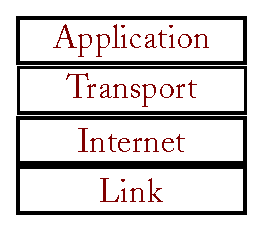
\includegraphics{layers.pdf}

\end{centering}
\end{figure}

\begin{figure}
\caption{As the Internet has evolved, researchers have created at
  least 40 mechanisms to govern resource allocation on the
  network---both entirely distributed schemes (``end-to-end'') and
  ones that include code running ``in-net.''}
\label{f:march}

\vspace{\baselineskip}

\begin{centering}
\noindent 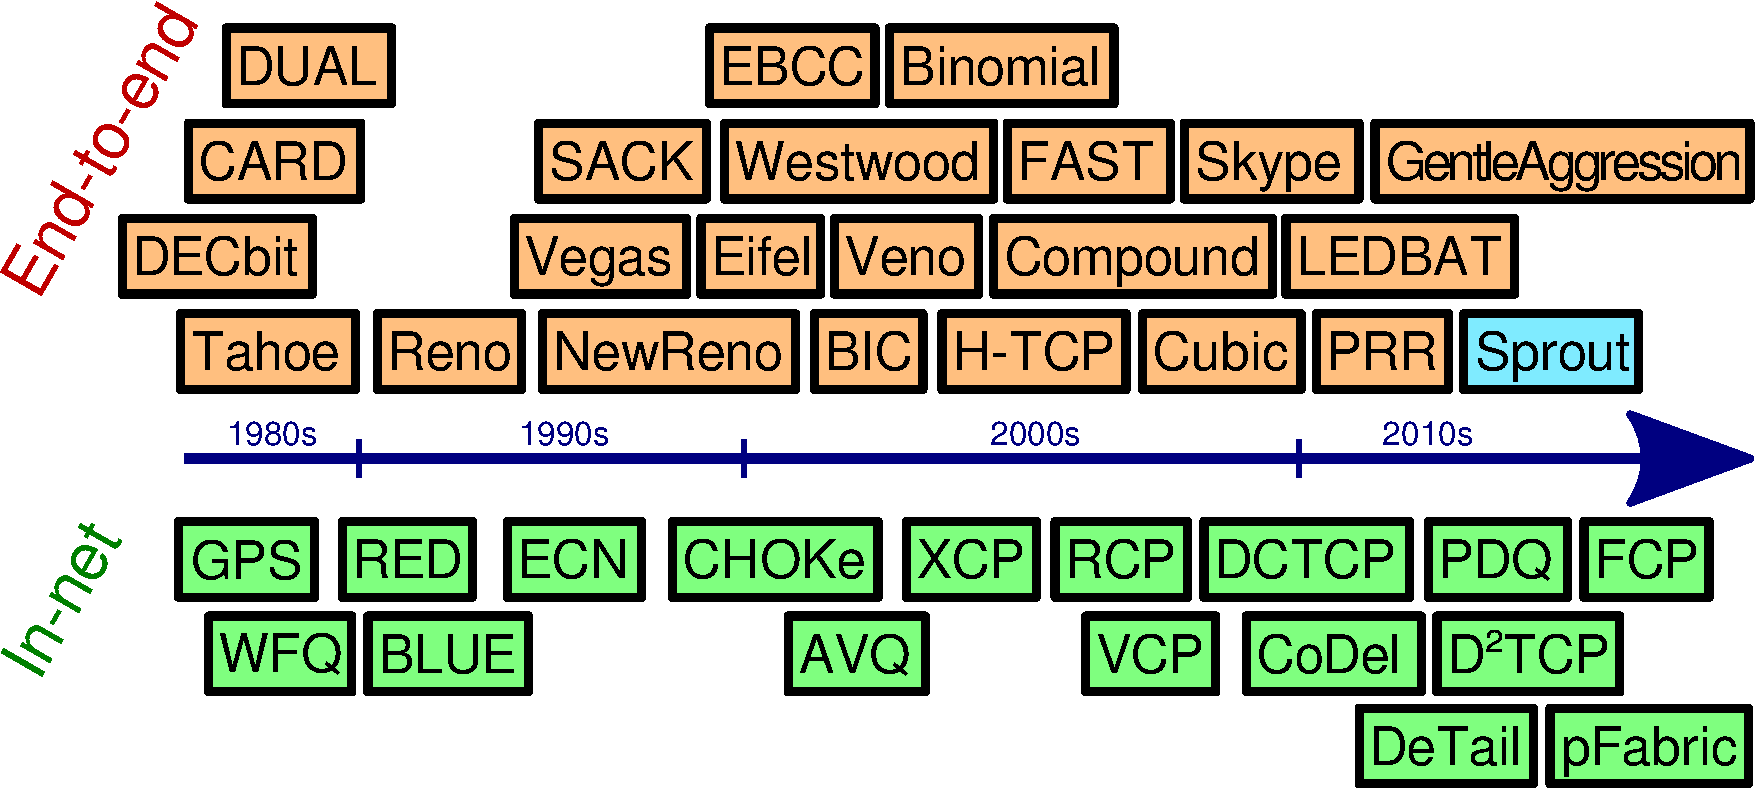
\includegraphics[width=\textwidth]{march2-all.pdf}

\end{centering}
\end{figure}

Over the last 25 years, the Internet has transformed from an academic
networking experiment into a global utility with billions of
users. With this rise, every layer of the Internet
``stack'' has seen dramatic change.

At the \textbf{link} layer, technologies that did not exist 25 years
ago now dominate---including wireless local-area networks (Wi-Fi),
cellular networks, datacenter interconnects, and transoceanic links
with high delay.

One layer up, at the \textbf{Internet} layer, mobility is now
ubiquitous. User devices regularly change their interface IP addresses
as they roam from network to network.

At the top layer of the Internet stack---the \textbf{application}
layer---none of the dominant applications of today existed 25 years
ago, including the World Wide Web and its short flows,
progressive-download video applications (e.g., YouTube and Netflix),
and real-time streaming video (e.g., Skype and Facetime).

The whole Internet has had to grapple with this continuous
evolution. How should the protocols of the \textbf{transport} layer,
sitting in the middle of the stack between the application and the
Internet, adapt to evolving application demands above them and
evolving networks below?

One legitimate answer is that these transport-layer protocols won't be
asked to adapt at all. If the network or applications evolve, our
current protocols will either be acceptable or not when run on the new
network or in service of the new application. If a protocol works
adequately, all is well. If not, we can simply stop using the protocol
and design a fresh one that matches the new circumstances.

This approach may sound wasteful, but it describes the extraordinarily
successful path taken over the last 25 years. Looking at just one
function of the transport layer---congestion control, the job of
dividing up the network's resources among contending
users---researchers have accommodated new applications and network
behaviors by devoting considerable effort to develop newer and newer
mechanisms, at least 40 in total so far (Figure \ref{f:march}).

Despite its demonstrable success, this approach can have downsides. In
defining transport-layer protocols by their \emph{mechanisms}---by the
actual behavior of endpoints or gateways that execute the
protocol---we leave implicit the assumptions that the mechanism makes
about the behavior of other layers and the policy that the mechanism
is built to pursue.

For contemporary mechanisms (e.g., TCP Cubic, the current default in
Linux), it's difficult to state the assumptions that the transport
makes about lower layers and to predict when those assumptions would
no longer hold. This presents a challenge for link-layer designers who
wish to design a new networking technology. Because of Cubic's
popularity, it can be a \emph{de facto} requirement that Cubic perform
well over any new network. In effect, this means that the designer of
the new link layer must try to satisfy Cubic's implicit assumptions in
order to achieve adequate performance.

This has led to the ``bufferbloat''\cite{bufferbloat} problem, which
comes from a link layer's attempt to hide losses from the transport,
on the grounds that the transport will assume that losses are a signal
to slow down. It has also led to a lack of parallelism in Internet
routing---flows only take one path, even if speedups might be
available by splitting flows across multiple routes---on the grounds
that the transport protocol probably assumes that out-of-order packets
are a pathology.

On the flip side, it is nontrivial to adjust the assumptions made by
the transport layer. There's no clear way to tweak the assumptions and
then retrace the same design process that was followed by a protocol's
designers, in order to explore the mechanism they would have produced
given a different starting point.

%\section{Showing our work in protocol design}

This thesis proposes essentially that approach to protocol design. The
transport layer should adapt to whatever the layers below may do, and
whatever the application above it wants done. Protocol designers
should specify the \emph{policy}---namely, what assumptions they want
to make about the network and what kind of performance the application
is interested in---and let computers worry about translating that into
the mechanism of congestion control.

By ``showing our work'' in this way, clearly enough for a computer to
recreate the same design, altering the assumptions is a matter of
changing the inputs to a computer program. This makes it easier for
adjacent layers to evolve. My colleagues and I have also found that
this approach can yield better performance than conventional,
human-designed protocols.

\section{Summary of results}

Over the last three years, my colleagues and I have built a series of
systems to explore this approach.

\subsection{Mosh (2011)}

\textbf{Mosh} (mobile shell)~\cite{mosh} is a replacement for SSH
(secure shell) in which the client and server each explicitly model
the dynamic contents of the text terminal. Unlike SSH, which transmits all
output from an application through a reliable TCP connection and
doesn't attempt to interpret the stream, Mosh's modeling allows it
to choose which data to send to the client when, in order to most
efficiently satisfy an explicit objective: update the client screen to
the current contents of the text terminal as efficiently as possible,
even across intermittent, roaming connectivity.

By having an explicit model of the user interface at both sides of the
connection, the Mosh client can predict the application's behavior in
response to user keystrokes and (if confident in its predictions)
speculatively display the result---generally an echoed keystroke or
cursor motion---before it has been confirmed by the server. In a
trace-based evaluation over 40 hours of real-world usage, Mosh was
able to successfully predict and immediately display the result of
\textbf{70\%} of user keystrokes.

Mosh is primarily a remote terminal application and is not further
discussed in this dissertation, but its design ideas---maintain an
explicit model at runtime, and pursue a stated objective on behalf of
the user---formed the basis of my subsequent work on
transport-protocol design.

\subsection{Sprout (2012)}

\textbf{Sprout} (Chapter~\ref{chap:sprout}) is a transport protocol
designed to carry high-throughput interactive traffic, such as a
videoconference, over a cellular network. Sprout includes an explicit
model of the dynamics of cellular networks and makes predictions about
future performance by inferring, with uncertainty, the current state
of the network and evolving the model forward. Its control
strategy---how much data to send at a given moment---is a function of
those predictions and of an explicit objective: maximize throughput,
but bound in-network delays to be at most 100~ms with high
probability.

In a trace-driven experimental evaluation (details in
\S\ref{sprout:eval}), Sprout gave 2-to-4 times the throughput and
7-to-9 times less delay than Skype, Apple Facetime, and Google
Hangouts:

\begin{center}
\noindent \begin{tabular}{|l|c|c|}
\hline
Sprout vs. & Avg.~speedup & Delay reduction \\
\hline
\hline
Skype & $2.2\times$ & $7.9\times$\\
Hangout & $4.4\times$ & $7.2\times$\\
Facetime & $1.9\times$ & $8.7\times$\\
\hline
Compound & $1.3\times$ & $4.8\times$\\
TCP Vegas & $1.1\times$ & $2.1\times$\\
LEDBAT & no change & $2.8\times$\\
Cubic & \cellcolor{red!20}$0.91\times$ & $79\times$\\
%\hline
%Cubic-CoDel & \cellcolor{red!20}$0.70\times$ & $1.6\times$ (0.50~s) \\
%CUBIC/CoDel & & \\
%Compound/CoDel & & \\
\hline
\end{tabular}

{\footnotesize Adapted from Figure~\ref{f:sproutcompe2e}.}

\end{center}

\subsection{Remy (2013--)}

\textbf{Remy} (Chapter~\ref{chap:remy}) generalizes Sprout to address
the classical problem of \emph{multi-agent} congestion control, where
independent users contend for the same limited network resource. Remy
is a protocol-design tool that takes, as input, a set of assumptions
about the uncertain network and workload, and an objective to pursue
on behalf of the application. Remy's computer-generated algorithms can
achieve higher performance and greater fairness than some
sophisticated human-designed schemes, including ones that put
intelligence inside the network.

On a simulated 15~Mbps fixed-rate link with eight senders contending and
an RTT of 150~ms, a computer-generated congestion-control algorithm
achieved the following improvements in median throughput and
reductions in median queueing delay over these existing protocols:

\begin{center}

\begin{tabular}{|l|c|c|}
\hline
Protocol & Median speedup & Median delay reduction \\
\hline
\hline
Compound & $2.1\times$ & $2.7\times$ \\
NewReno & $2.6\times$ & $2.2\times$ \\
Cubic & $1.7\times$ & $3.4\times$ \\
Vegas & $3.1\times$ & $1.2\times$ \\
\hline
Cubic/sfqCoDel & $1.4\times$ & $7.8\times$ \\
XCP & $1.4\times$ & $4.3\times$ \\
\hline
\end{tabular}

{\footnotesize Adapted from \S\ref{sec:remyresults}.}

\end{center}

Once we had a computerized protocol designer, we explored using it as
a tool to gain understanding about the problem of congestion control.
How easy is it to ``learn'' a network protocol to achieve desired
goals, given a necessarily imperfect model of the networks where it
ultimately will be deployed? Is there a tradeoff between the
performance of an algorithm now---if optimized for a very specific
network---versus the protocol's ability to perform adequately as the
network evolves? What is the cost of compatibility with existing TCP
congestion-control mechanisms?

Our experimentats into these questions of ``learnability'' are reported
in Chapter~\ref{chap:learnability}. We found:

\begin{itemize}

\item Weak evidence of a tradeoff between the breadth of the operating
  range of a computer-generated protocol and its performance.

\item Modeling a two-bottleneck network as a single bottleneck hurt
  performance mildly.

\item Building in ``TCP-awareness'' to a computer-generated protocol
  helped in the case when cross-traffic was governed by TCP, but made
  the protocol more aggressive (and consequently increased delay) when
  it was contending only against other cross-traffic generated by the
  same algorithm.

\end{itemize}

\chapter{Domino: Programming Stateful Algorithms on a Router's Data Plane}
\label{chap:domino}

This chapter focuses on the hardware and software required to program {\em
stateful data-plane algorithms} on high-speed routers. These algorithms process
and transform packets, reading and writing state in the router. Examples
include active queue management~\cite{red,avq,codel}, congestion control with
router feedback~\cite{xcp, rcp}, network measurement~\cite{opensketch,
bitmap_george}, and data-plane traffic engineering~\cite{conga, flowlet}.

As explained earlier (\S\ref{s:intro_background} and
Figure~\ref{fig:router_algos}), such algorithms are either not available on
high-end routers or are hardwired into fixed-function routers where they cannot
be modified. In other words, there is no way to program a new algorithm or
modify the algorithmic logic of an old one on a high-speed router. While
high-speed programmable router chips~\cite{flexpipe, xpliant} are available,
their programmability is largely restricted to {\em stateless} tasks such as
packet forwarding (\S\ref{ss:prog_router_chips}). By contrast to packet
forwarding, which doesn't modify state in the data plane, many data-plane
algorithms create and modify {\em algorithmic state} in the router as part of
packet processing.

The central question of this chapter is: {\em how do we enable programmable
stateful processing on a high-speed router?} In more detail, what is the right
programming model for stateful algorithms, what is the underlying instruction
set, and how do we compile from the programming model to the instruction set?

In answering these questions, this chapter makes three new contributions.
First, {\em \absmachine}, a machine model for programmable line-rate
routers~(\S\ref{s:absmachine}).  \absmachine is inspired by existing
programmable router chips, but extends them with functionality required for
state modifications in the router's ASIC.  Specifically, \absmachine models two
important constraints (\S\ref{s:atomConstraints}) for stateful line-rate
operations: the inability to share state between different packet-processing
units, and the requirement that any router state modifications be visible to
the next packet entering the router. Based on these constraints, we introduce
{\em atoms} to represent a programmable router's packet-processing units.

Second, a new abstraction to program and implement data-plane algorithms: a
{\em packet transaction} (\S\ref{s:transactions}). A packet transaction is a
sequential code block that is atomic and isolated from other such code blocks.
Packet transactions provide programmers with the illusion that the
transaction's body executes serially from start to finish on each packet, with
no overlap in packet processing across packets---akin to an infinitely fast
single-threaded processor carrying out packet processing on each packet. The
code within a packet transaction is written in {\em \pktlanguage{}}, a new
imperative domain-specific language (DSL) for (\S\ref{s:transactions}).
\pktlanguage is  to our knowledge the first to offer such a high-level
programming abstraction for line-rate routers.

Packet transactions let the programmer focus on the operations needed for each
packet without worrying about other concurrent packets. Packet transactions
have an \textit{all-or-nothing} guarantee: all packet transactions accepted by
the packet transactions compiler will run at line rate, or be rejected.  There
is no ``slippery slope'' of running network algorithms at lower speeds as with
network processors or software routers: when compiled, a packet transaction
runs at the router's line rate, or not at all.  Performance is not just
predictable, but guaranteed.

Third, {\em a compiler from \pktlanguage packet transactions to a \absmachine
target}~(\S\ref{s:compiler}). The \pktlanguage compiler extracts {\em codelets}
from  transactions: code fragments, which if executed atomically, guarantee a
packet transaction's semantics. It then uses program
synthesis~\cite{sketch_asplos} to map codelets to atoms, rejecting the
transaction if the atom cannot execute the codelet.

We evaluate \pktlanguage's expressiveness by programming a variety of
data-plane algorithms (Table~\ref{tab:algos}) in \pktlanguage and compare with
P4. We find that \pktlanguage provides a more concise and natural programming
model for stateful data-plane algorithms.  Next, we design a set of small set
of atoms that can express these algorithms (\S\ref{ss:targets}).  We show that
compiler targets with these atoms are feasible in a 32-nm standard-cell library
with $< 2\%$ cost in area relative to a 200 \si{\milli\metre\squared} baseline
router chip~\cite{gibb_parsing}.  Finally, we compile data-plane algorithms
written in \pktlanguage to these targets (\S\ref{domino_ss:compiler}) to show
how a target's atoms determine the algorithms it can support. We also distill
with several lessons for programmable router design (\S\ref{ss:lessons}) based
on our experience with \pktlanguage.
%TODO: Tone down comparison with P4 here. That's not the point here.

Code for the \pktlanguage compiler, the \absmachine machine model, and the code
examples listed in Table~\ref{tab:algos} is available at
\url{http://web.mit.edu/domino}.

\section{A machine model for line-rate routers}
\label{s:absmachine}
\begin{figure}[!t]
  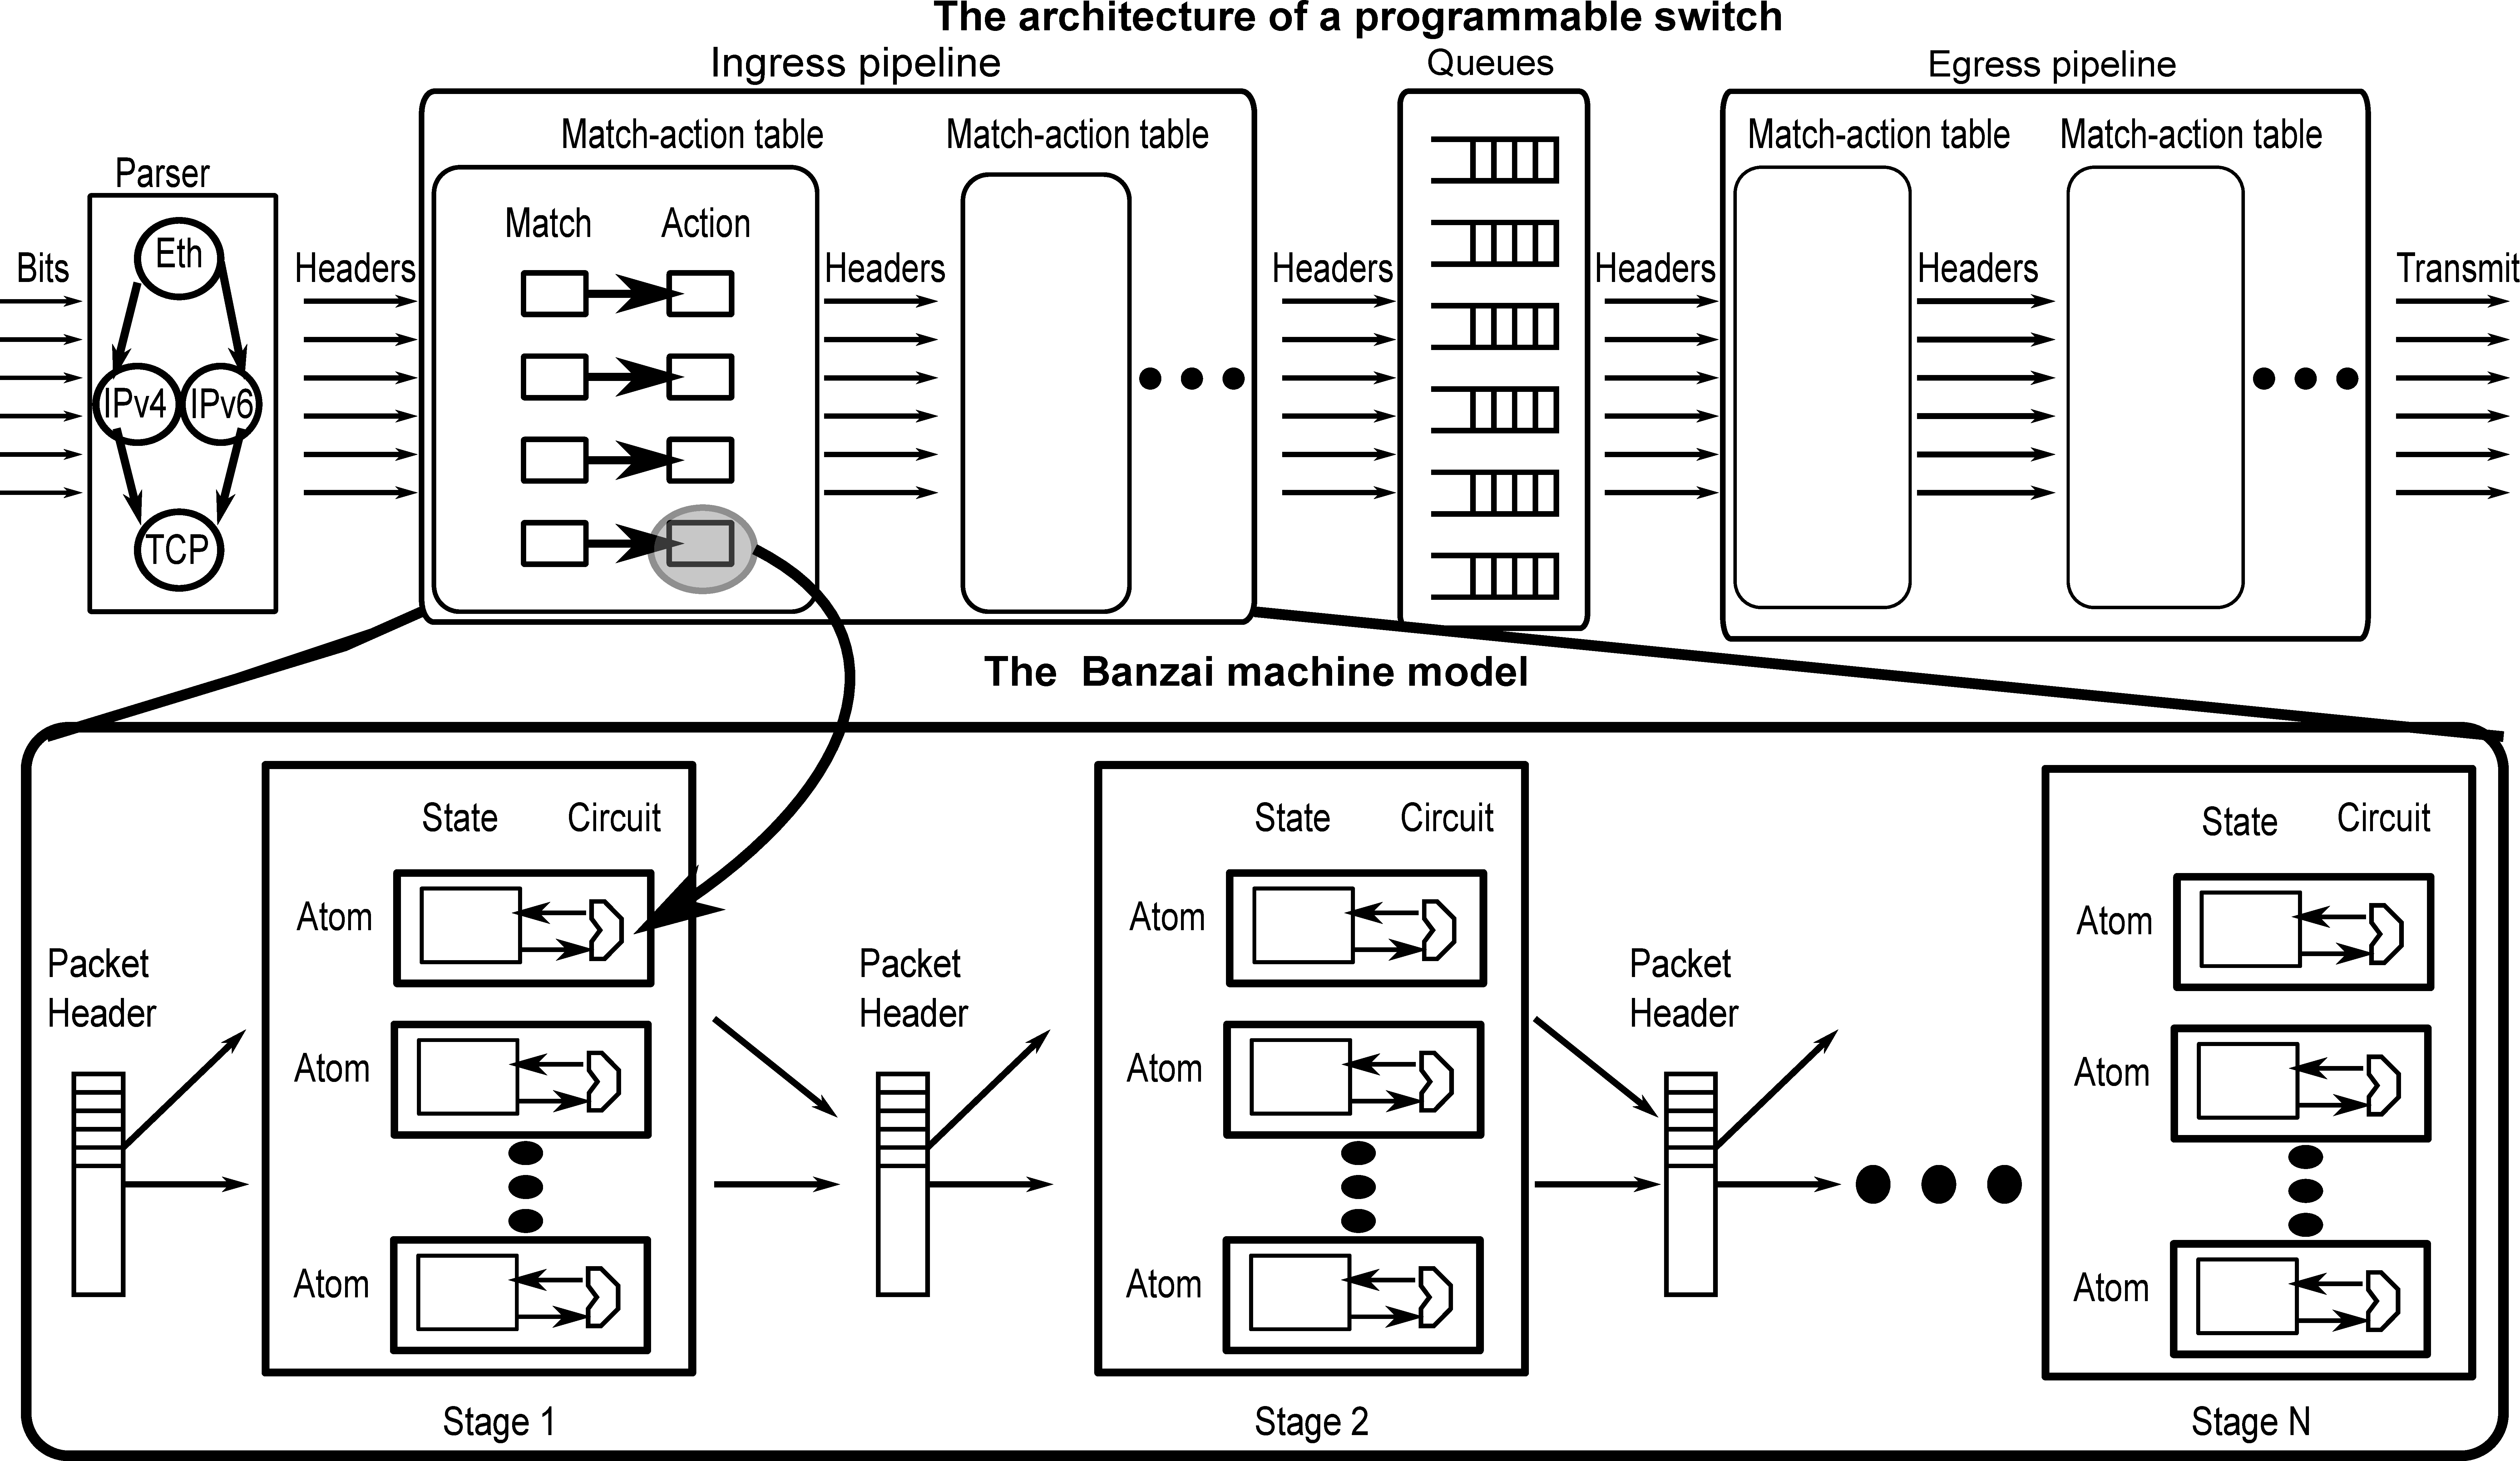
\includegraphics[width=\textwidth]{domino_banzai.pdf}
  \caption{\absmachine models the ingress or egress pipeline of a
  programmable router. An atom corresponds to an action in a match-action
  table. Internally, an atom contains local state and a digital circuit 
  modifying this state. Figure~\ref{fig:atom} details an atom.}
  \label{domino_fig:router}
\end{figure}

\absmachine is a machine model for programmable line-rate routers that serves
as the compiler target for \pktlanguage.  \absmachine is inspired by recent
programmable router architectures such as Barefoot Networks' Tofino~\cite{tofino},
Intel's FlexPipe~\cite{flexpipe}, and Cavium's XPliant Packet
Architecture~\cite{xpliant}. \absmachine abstracts these architectures and
extends them with stateful processing units to implement data-plane algorithms.
These processing units, called {\em atoms}, model atomic operations
that are natively supported by a programmable line-rate router.

\subsection{Background: programmable routers}
Packets arriving at a router~(top half of Figure~\ref{domino_fig:router}) are parsed
by a programmable parser that turns packets into header fields. These header
fields are first processed by an ingress pipeline consisting of match-action
tables arranged in stages. Processing a packet at a stage may modify its header
fields, through match-action rules, as well as some persistent state at that
stage, e.g., packet counters. After the ingress pipeline, the packet is
queued. Once the scheduler dequeues the packet, it is processed by a
similar egress pipeline before it is transmitted.

To reduce chip area, there is only one ingress and one egress pipeline.  This
single pipeline is shared across all router ports and handles aggregate traffic
belonging to all ports, at all packet sizes.  For instance, a 64-port router
with a line rate of 10 Gbit/s per port and a minimum packet size of 64 bytes
needs to process around a billion packets per second, after accounting for
minimum inter-packet gaps~\cite{rmt}.  Equivalently, the pipeline runs at 1
GHz, and pipeline stages process a packet every clock cycle (1 ns).  We assume
one packet per clock cycle throughout the paper, and for concreteness, a
1 GHz clock frequency.

Having to process a packet every clock cycle in each stage constrains
the operations that can be performed on each packet. In particular, any packet
operation that modifies state visible to the next packet {\em must} finish
execution in a single clock cycle (\S\ref{ss:atoms} shows why). Because
of this restriction, programmable routering chips provide a small set of
processing units or primitives for manipulating packets and state in a stage,
unlike software routers. These primitives determine which algorithms
run on the router at line rate.

The challenge for us is to develop primitives that allow a broad range of
data-plane algorithms to be implemented, and to build a compiler to map a
user-friendly description of an algorithm to the primitives provided by a
router.

\subsection{The \absmachine machine model}

\absmachine (the bottom half of Figure~\ref{domino_fig:router}) models
the ingress or egress router pipeline.  It models the
computation within a match-action table in a stage (i.e., the action half of
the match-action table), but not how packets are matched (e.g., direct or
ternary). \absmachine does not model packet parsing and assumes
that packets arriving to \absmachine are already parsed.
%We discuss how to embed \absmachine in a standard match-action
%pipeline in \S\ref{ss:guards}.  

 Concretely, \absmachine is a feed-forward pipeline\footnote{It is hard to
physically route backward-flowing wires that would be required for feedback.}
consisting of a number of stages executing synchronously on every clock cycle.
Each stage processes one packet every clock cycle and hands it off to the next.
Unlike a CPU pipeline, which occasionally experiences pipeline stalls,
\absmachine's pipeline is deterministic, never stalls, and always sustains line
rate. However, relative to a CPU pipeline, \absmachine is restricted in the
operations it supports (\S\ref{s:atomConstraints}).

\subsection{Atoms: \absmachine's processing units}
\label{ss:atoms}
 An {\em atom} is an atomic unit of packet processing supported natively by a
\absmachine machine, and the atoms within a \absmachine machine form its
instruction set. Each pipeline stage in \absmachine contains a vector of atoms.
Atoms in this vector modify mutually exclusive sections of the same packet
header in parallel in every clock cycle, and process a new packet header every
clock cycle.

In addition to packet headers, atoms may modify persistent state on the router
to implement stateful data-plane algorithms. To support such algorithms at
line-rate, the atoms for a \absmachine machine need to be substantially richer
(Table~\ref{tab:templates}) than the simple RISC-like stateless instruction
sets for programmable routers today~\cite{rmt}. We explain why below.

Suppose we need to atomically increment a router counter to count packets. One
approach is hardware support for three simple single-cycle operations:
\textit{read} the counter from memory in the first clock cycle, \textit{add}
one in the next, and \textit{write} it to memory in the third.  This approach,
however, does not provide atomicity. To see why, suppose packet $A$ increments
the counter from 0 to 1 by executing its read, add, and write at clock cycles
1, 2, and 3 respectively.  If packet $B$ issues its read at time 2, it will
increment the counter again from 0 to 1, when it should be incremented to 2.

Locks over the shared counter are a potential solution.  However, locking
causes packet $B$ to wait during packet $A$'s increment, and the router no
longer sustains the line rate of one packet every clock cycle. CPUs employ
micro-architectural techniques such as operand forwarding for this
problem. But these techniques still suffer pipeline stalls, which prevents
line-rate performance from being achieved.

\absmachine provides an atomic increment operation at line rate with an {\em
atom} to read a counter, increment it, and write it back in a single stage within
one clock cycle. It uses the same approach of reading, modifying, and writing
back to implement other stateful atomic operations at line rate.

Unlike stateful atomic operations, stateless atomic operations are easier to
support with simple packet-field arithmetic.  Consider, for
instance, the operation {\tt pkt.f1 = pkt.f2 + pkt.f3 - pkt.f4}.  This
operation does not modify any persistent router state and only accesses packet
fields. It can be implemented atomically by using two atoms: one atom to add
fields f2 and f3 in one pipeline stage, and another to subtract f4 from the
result in the next. An instruction set designer can provide {\em simple}
stateless instructions operating on a pair of packet fields. These instructions can then be
composed into larger stateless operations, without designing atoms specifically
for each stateless operation.

\medskip
\noindent
\textbf{Representing atoms.}
An atom is represented by a body of sequential code that captures the atom's
behavior. It may also contain internal state local to the atom. An atom
completes execution of this entire body of code, modifying a packet and any
internal state before processing the next packet. The designer of a
programmable router would develop these atoms, and expose them to a router
compiler as the programmable router's instruction set, e.g.,
Table~\ref{tab:templates}.

Using this representation, a router counter that wraps around at a
value of 100 can be written as the atom:\footnote{We use {\tt p.x} to
  represent field {\tt x} within a packet {\tt p} and {\tt x} to
  represent a state variable {\tt x} that persists across packets.}
\begin{lstlisting}[style=customc, numbers=none, frame=none]
if (counter < 99)
  counter++;
else
  counter = 0;
\end{lstlisting}

Similarly, a stateless operation like setting a packet field to a constant
value can be written as the atom:
\begin{lstlisting}[style=customc, numbers=none, frame=none]
  pkt.field = value;
\end{lstlisting}

\subsection{Constraints for line-rate operation}
\label{s:atomConstraints}

\medskip
\noindent
\textbf{Memory limits.} State in \absmachine is local to each atom.  It can
neither be shared by atoms within a stage, nor atoms across stages. This is
because building multi-ported memories accessible to multiple atoms is
technically challenging and consumes additional chip area. However, state can
be read into a packet header in one stage, for subsequent use by a downstream
stage\footnote{Figure~\ref{fig:flowlet_pipeline} shows an example. {\tt
last\_time} is read into {\tt pkt.last\_time} in stage 2, for subsequent use by stage 3.}.  But, the \absmachine pipeline is
feed-forward, so state can only be carried forward, not backward.

\medskip
\noindent
\textbf{Computational limits.} Atoms need to execute atomically from one packet
to the next, so any state internal to the atom must be updated
before the next packet arrives.  Because packets may be separated by as little
as one clock cycle, we mandate that atom bodies finish execution within one
clock cycle, and constrain atom bodies to do so.

We constrain atom bodies by defining {\it atom templates}
(\S\ref{ss:code_gen}).  An atom template is a program with configurable
parameters that terminates within a clock cycle and specifies the atom's
behavior.  An example is an ALU with a restricted set of primitive operations
(Figure~\ref{fig:alu_diag}).

% Atom templates allow us to create
%and experiment with \absmachine machines with different atoms.

%As programmable
%routers evolve, we expect that atoms will evolve as well, but constrained by
%the clock-cycle requirement.

\begin{figure}[h]
  \begin{subfigure}{0.5\columnwidth}
  \centering
  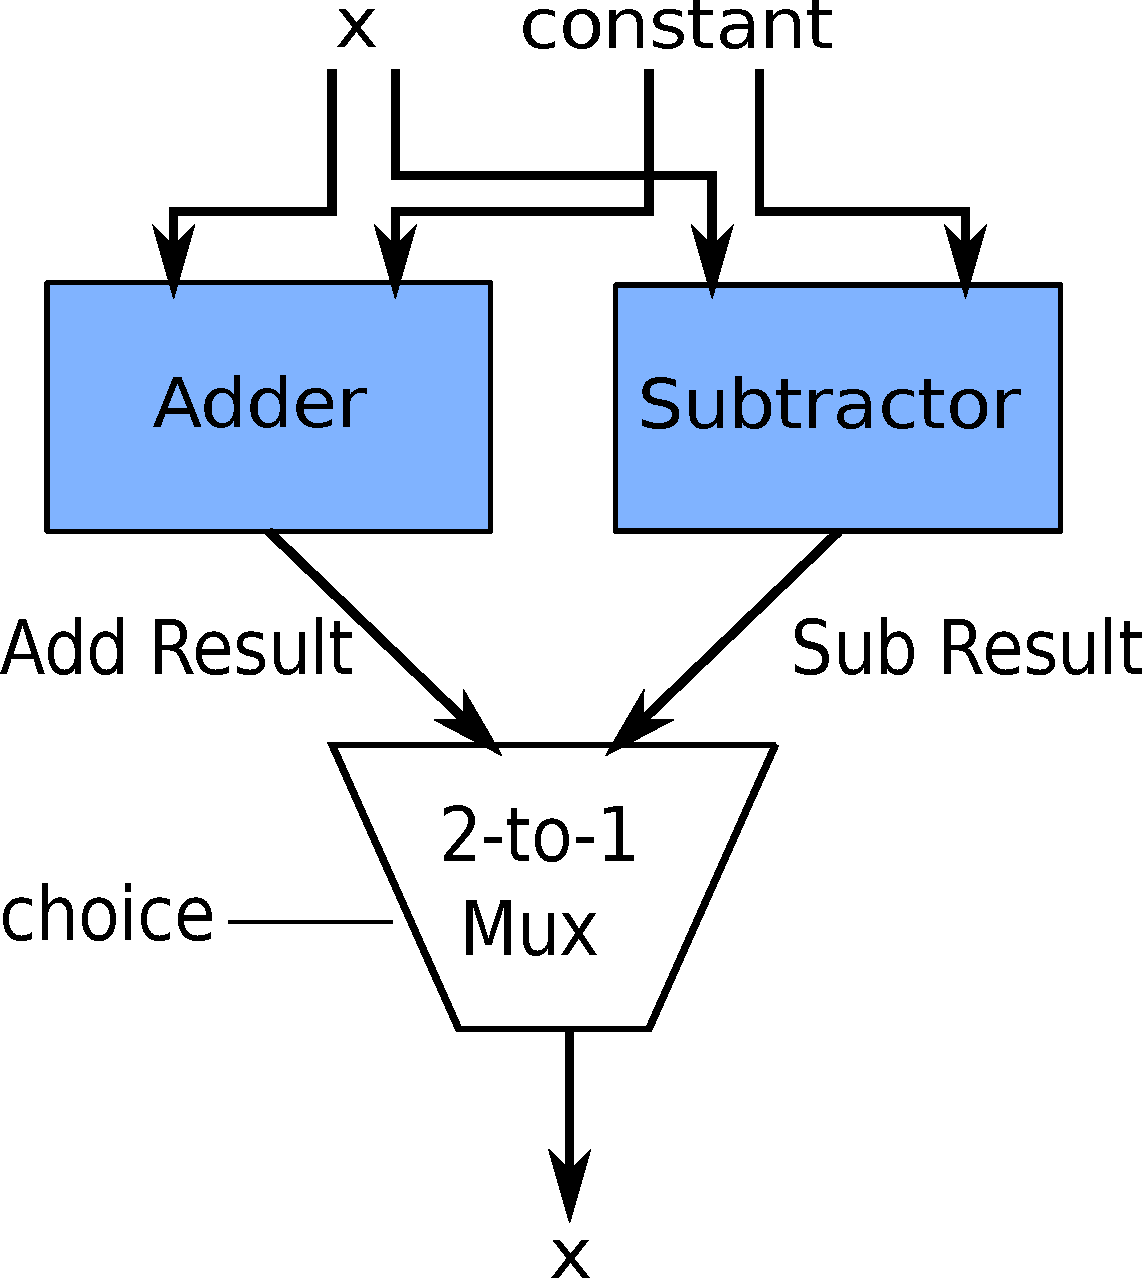
\includegraphics[width=0.5\textwidth]{domino_circuit.pdf}
  \caption{Circuit for the atom}
  \label{fig:alu_diag}
  \end{subfigure}
  \hspace{0.1\columnwidth}
  \begin{subfigure}{0.3\columnwidth}
  \begin{lstlisting}[belowskip=-0.8 \baselineskip]
  bit choice = ??;
  int constant = ??;
  if (choice) {
    x = x + constant;
  } else {
    x = x - constant;
  }
  \end{lstlisting}
  \hspace{0.1\columnwidth}
  \caption{Atom template}
  %Each ``??(n)'' represents a hole that can be filled in with values in $[0, 2^n -1]$.}
  \label{fig:alu_in_sketch}
  \end{subfigure}
  \caption{An atom and its template. The atom above can add or subtract a constant from a state
  variable {\tt x} based on two configurable parameters, {\tt constant} and {\tt choice}.}
  \label{fig:atom}
\end{figure}

\medskip
\noindent
\textbf{Resource limits.} We also limit the number of atoms in each stage
(\textit{pipeline width}) and the number of stages in the pipeline
(\textit{pipeline depth}). This is similar to limits on the number of stages,
tables per stage, and memory per stage in programmable router
architectures~\cite{lavanya_compiler}.

\subsection{What can \absmachine not do?}
\label{domino_ss:limitations}

\absmachine is a good fit for data-plane algorithms that modify a small set of
packet headers and carry out small amounts of computation per packet.
Data-plane algorithms like deep packet inspection and WAN optimization require
a router to parse and process the packet payload as well---effectively parsing
a large ``header'' consisting of each byte in the payload. This is challenging
at line rates of 1 GHz, and such algorithms are best left to CPUs~\cite{e2}.
Some algorithms require complex computations, but not on every packet, e.g., a
measurement algorithm that periodically scans a large table to perform garbage
collection.  \absmachine's atoms model small operations that occur on every
packet, and are unsuitable for such operations that span many clock cycles.

\section{Packet transactions}
\label{s:transactions}

\begin{figure}[!t]
\begin{subfigure}{0.6\textwidth}
\begin{small}
\begin{lstlisting}[style=customc]
#define NUM_FLOWLETS    8000
#define THRESH          5
#define NUM_HOPS        10

struct Packet {
  int sport;
  int dport;
  int new_hop;
  int arrival;
  int next_hop;
  int id; // array index
};

int last_time [NUM_FLOWLETS] = {0};
int saved_hop [NUM_FLOWLETS] = {0};

void flowlet(struct Packet pkt) {
  pkt.new_hop = hash3(pkt.sport,
                      pkt.dport,
                      pkt.arrival)
                % NUM_HOPS;

  pkt.id  = hash2(pkt.sport,
                  pkt.dport)
            % NUM_FLOWLETS;

  if (pkt.arrival - last_time[pkt.id] @\label{line:ifStart}@
      > THRESH)
  { saved_hop[pkt.id] = pkt.new_hop; } @\label{line:ifEnd}@

  last_time[pkt.id] = pkt.arrival;
  pkt.next_hop = saved_hop[pkt.id];
}
\end{lstlisting}
\end{small}
\caption{Flowlet switching written in \pktlanguage}
\label{fig:flowlet_code}
\end{subfigure}
\begin{subfigure}{0.4\textwidth}
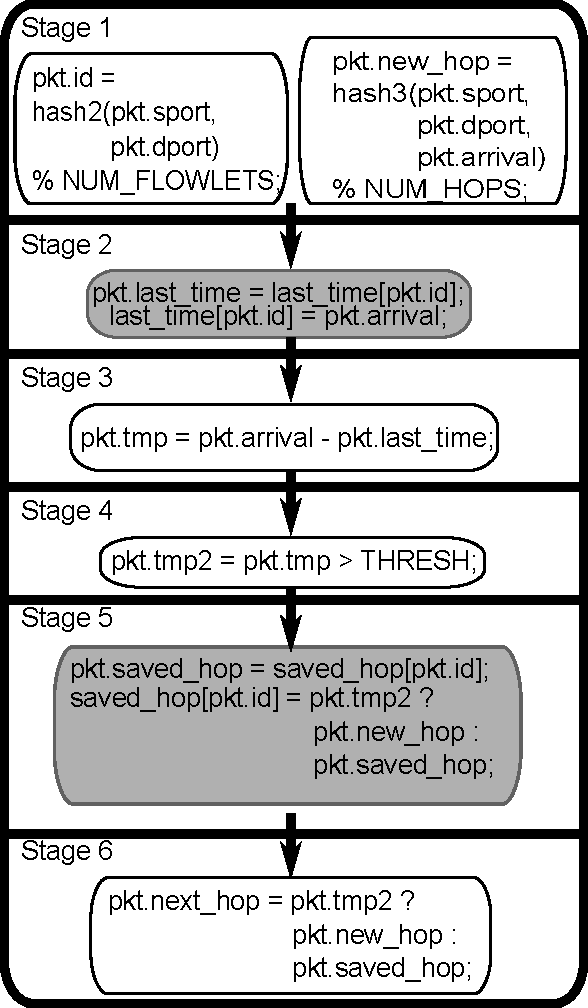
\includegraphics[width=\columnwidth]{domino_pipe.pdf}
\caption{6-stage \absmachine pipeline for flowlet
switching.  Control flows from top to bottom. Stateful atoms are in grey.}
\label{fig:flowlet_pipeline}
\end{subfigure}
\caption{Programming flowlet switching in \pktlanguage}
\vspace{-0.35in}
\end{figure}

A programmer programs a data-plane algorithm by writing it as
a packet transaction in \pktlanguage (Figure~\ref{fig:flowlet_code}).  The
\pktlanguage compiler then compiles this transaction to an atom pipeline for a
\absmachine machine (Figure~\ref{fig:flowlet_pipeline}). We first describe
packet transactions in greater detail by walking through an example
(\S\ref{ss:flowlet}). Next, we discuss language constraints in \pktlanguage
(\S\ref{ss:constraints}) informed by line-rate routers.  We then discuss
triggering packet transactions (\S\ref{ss:guards}) and handling multiple
transactions (\S\ref{ss:multiple}).

\subsection{\pktlanguage by example}
\label{ss:flowlet}

We use flowlet routering~\cite{flowlets} as our running example. Flowlet
routering is a load-balancing algorithm that sends bursts of packets, called
flowlets, from a TCP flow on a randomly chosen next hop, provided the bursts
are separated by a large enough time interval to ensure packets do not arrive
out of order at a TCP receiver. For ease of exposition, we use only the source
and destination ports in the hash function that randomly computes the next hop
for flowlet routering.
%it is easy to extend it to the full 5-tuple.

Figure~\ref{fig:flowlet_code} shows flowlet routering in \pktlanguage and
demonstrates its core language constructs. All packet processing happens in the
context of a packet transaction (the function \texttt{flowlet} starting at line
17). The function's argument type {\tt Packet} declares the fields in a packet
(lines 5--12)\footnote{A field is either a packet header, e.g.,
source port ({\tt sport}) and destination port ({\tt dport}), or packet
 metadata ({\tt id}).} that can be referenced by the function body (lines
18--32).  The function body can also modify persistent router state using
global variables (e.g., \texttt{last\_time} and \texttt{saved\_hop} on lines 14
and 15, respectively). The function body may use \textit{intrinsics} such as
\texttt{hash2} on line 23 to directly access hardware accelerators on the
router such as hash generators.  The \pktlanguage compiler uses an intrinsic's
signature to analyze read/write dependencies (\S\ref{ss:pipelining}), but otherwise considers it a blackbox.

\medskip
\noindent
\textbf{Packet transaction semantics.}
Semantically, the programmer views the router as invoking the packet transaction
serially in the order in which packets arrive, with no concurrent packet
processing.  Put differently, the packet transaction modifies the passed-in
packet argument and runs to completion, before starting on the next packet.
These semantics allow the programmer to program under the illusion that a
single, extremely fast, processor is serially executing the packet processing code for
all packets. The programmer doesn't worry about parallelizing the code within
and across pipeline stages to run at line rate.

\subsection{The \pktlanguage language}
\label{ss:constraints}
\pktlanguage's syntax (Figure~\ref{fig:grammar}) is similar to C, but with
several constraints (Table~\ref{tab:restrict}).  These constraints are required
for deterministic performance.  Memory allocation, unbounded iteration counts,
and unstructured control flow cause variable performance, which may prevent an
algorithm from achieving line rate. Additionally, within a \pktlanguage transaction, 
each array can only be accessed using a single packet field, and repeated accesses to the 
same array are allowed only if that packet field is unmodified between accesses.
%array modifications by mandating that a single execution of a transaction (the
%execution of a transaction for a single packet) can access only one entry in an
%array.

For example, all read and write accesses to \texttt{last\_time} use the
index \texttt{pkt.id}. \texttt{pkt.id} is not modified during the
course of a single transaction execution (single packet); it only changes between executions
(packets).  This restriction on arrays mirrors restrictions on the stateful memories
attached to atoms (\S\ref{s:atomConstraints}), which require multiple ports to
support distinct read and write addresses every clock cycle.

\begin{table}
  \begin{tabular}{p{0.95\columnwidth}}
   No iteration (while, for, do-while).\\
   No unstructured control flow (goto, break, continue).\\
   No heap, dynamic memory allocation, or pointers.\\
   At most one location in each array is accessed by a single execution of a transaction. \\
   No access to unparsed portions of the packet (payload).\\
  \end{tabular}
  \caption{Restrictions in \pktlanguage}
  \label{tab:restrict}
\end{table}

\begin{figure}
\newcommand{\sep}{~|~}
\begin{small}
\begin{eqnarray*}
l \in \text{literals} \quad v \in \text{variables} \quad &bop& \in \text{binary ops} \quad
uop \in \text{unary ops} \\
%
e \in \text{expressions} &::=& e.f \sep l \sep v \sep e~bop~e \sep uop~e \sep e[d.f] \sep \\
                   & &   f(e_1, e_2, \ldots) \\
%
s \in \text{statements} &::=& e = e \sep {\tt if}~(e)~\{ s \}~{\tt else}~ \{ s \} \sep s~;~s \\
%
t \in \text{packet txns} &::=& name(v) \{ s \} \\
%
%vlist \in varList &::=& var;vlist \sep vlist \\
%
d \in \text{packet decls} &::=& \{ v_1, v_2, \ldots \} \\
%
sv \in \text{state var inits} &::=& v = e \sep sv~;~sv \\
%
p \in \text{\pktlanguage programs} &::=& \{ d ; sv; t \}
\end{eqnarray*}
\end{small}
\caption{\pktlanguage grammar. Type annotations (void, struct, int, and Packet) are elided for simplicity.}
\label{fig:grammar}
\end{figure}


\subsection{Triggering packet transactions}
\label{ss:guards}
Packet transactions specify \textit{how} to process packet headers and state.  To
specify {\em when} to run packet transactions, programmers use {\em guards}:
predicates on packet fields that trigger a transaction if a packet
matches the guard. For example, {\tt (pkt.tcp\_dst\_port == 80)} would
trigger heavy-hitter detection~\cite{opensketch} on packets with TCP
destination port 80.

Guards can be realized using an exact match in a match-action table, with the
actions being the atoms compiled from a packet transaction. Guards
can take various forms, e.g., exact, ternary, longest-prefix, and range-based
matches, depending on the matches supported by the match-action
pipeline. Because guards map straightforwardly to the match key in a
match-action table, we focus only on compiling packet transactions in this paper.

\subsection{Handling multiple transactions}
\label{ss:multiple}
So far, we have discussed a single packet transaction corresponding to a single
data-plane algorithm. In practice, a router would run multiple data-plane
algorithms, each processing its own subset of packets. To address this, we
envision a policy language that specifies pairs of guards and transactions.
Realizing a policy is straightforward when all guards are disjoint. When guards
overlap, multiple transactions need to execute on the same subset of packets,
requiring a mechanism to compose transactions.

One composition semantics is to run the two transactions one after another
sequentially in a user-specified order. This can be achieved by concatenating
the two transaction bodies to create a larger transaction.  We leave a detailed
exploration of multiple transactions to future work, and focus only on
compiling a single packet transaction here.

\section{The Domino compiler}
\label{s:compiler}

The \pktlanguage compiler translates \pktlanguage programs to \absmachine
targets. The compiler provides an {\em all-or-nothing model}: if compilation
succeeds, the program will run at line rate on the target with packet
transaction semantics. Otherwise, if the program cannot run at line rate, it
will not compile. This all-or-nothing model trades off diminished
programmability for guaranteed line-rate performance, in contrast to software
routers that provide greater flexibility, but lower and unpredictable run-time
performance~\cite{dobrescu2012}.

The \pktlanguage compiler has three passes (Figure~\ref{fig:passes}), which we
illustrate using the flowlet switching example.  \textit{Preprocessing}
(\S\ref{ss:preprocessing}) simplifies packet transactions into a simpler
three-address code form~\cite{tac}.
\textit{Pipelining} (\S\ref{ss:pipelining}) transforms preprocessed code into
code for a \textit{Pipelined Virtual Switch Machine (PVSM)}, an intermediate
representation that models a switch pipeline with no computational or resource
limits. \textit{Code generation} (\S\ref{ss:code_gen}) transforms this
intermediate representation into configuration for a \absmachine machine, given
the machine's computational and resource limits (\S\ref{s:atomConstraints}),
and rejects the program if it can not run at line rate.  The \pktlanguage
compiler uses many existing compilation techniques, but adapts
them in important ways for line-rate switches (\S\ref{ss:related_compiler}).

\begin{figure}[!t]
  \centering
  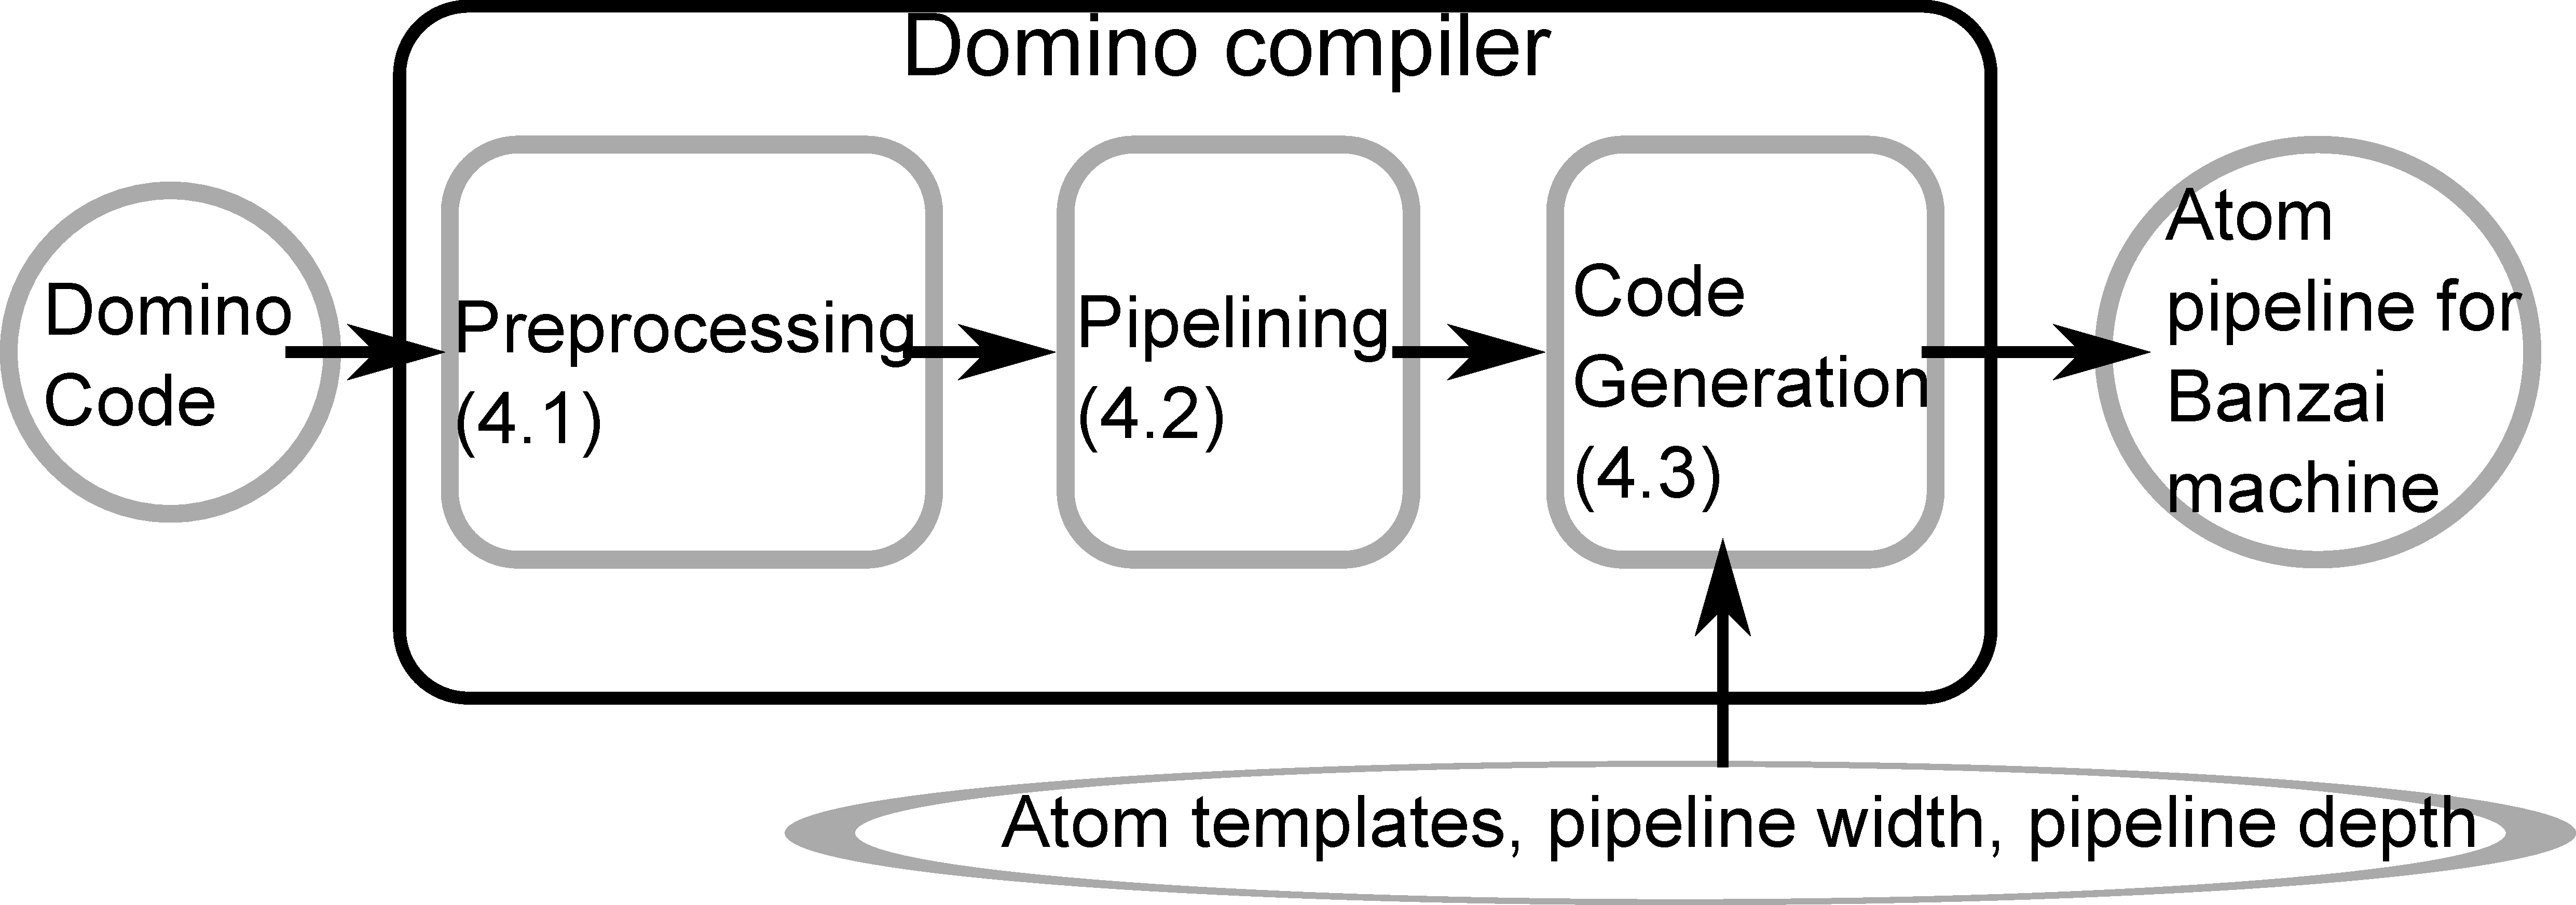
\includegraphics[width=0.75\columnwidth]{domino_compiler.pdf}
  \caption{Passes in the \pktlanguage compiler}
  \label{fig:passes}
\end{figure}

\subsection{Preprocessing}
\label{ss:preprocessing}

\medskip
\noindent
\textbf{Branch removal.} A packet transaction's body can contain (potentially
nested) branches (e.g., Lines~\ref{line:ifStart} to \ref{line:ifEnd} in
Figure~\ref{fig:flowlet_code}).  Branches alter control flow and complicate
dependency analysis, i.e.,  whether a statement should precede another.  We
transform branches into conditional assignments, starting from the innermost
\texttt{if} and proceeding outwards (Figure~\ref{fig:if_convert}).  This turns
the transaction body into straight-line code with no branches, which simplifies
dependency analysis during pipelining (\S\ref{ss:pipelining}).

\medskip
\noindent
\textbf{Rewriting state variable operations.} We now identify state variables
in a packet transaction, e.g., \texttt{last\_time} and \texttt{saved\_hop} in
Figure~\ref{fig:flowlet_code}.  For each state variable, we create a
\textit{read flank} to read the variable into a temporary packet field.
For an array, we also move the index expression into the read flank using the
fact that only one array index is accessed per packet (\S\ref{ss:constraints}).
Within the packet transaction, we replace the state variable with the temporary
packet field, and create a \textit{write flank} to write this temporary packet
field back to the state variable~(Figure~\ref{fig:stateful_flanks}). After
this, the only operations on state variables are reads and writes; all
arithmetic happens on packet fields. Restricting stateful operations simplifies
handling of state during pipelining (\S\ref{ss:pipelining}).

\medskip
\noindent
\textbf{Converting to static single-assignment form.} We next convert the code
to static single-assignment form (SSA)~\cite{ssa}, where every packet field is
assigned exactly once. We do this by replacing every assignment to a packet
field with a new packet field and propagating this until the next assignment to
the same field~(Figure~\ref{fig:ssa}) .  Because fields are assigned once, SSA
removes Write-After-Read and Write-After-Write dependencies.  Only
Read-After-Write dependencies remain during pipelining (\S\ref{ss:pipelining}).

\medskip
\noindent
\textbf{Flattening to three-address code.} Three-address code is a
representation where all instructions are either reads/writes into state
variables or operations on packet fields of the form \texttt{pkt.f1 = pkt.f2 op
pkt.f3}, where \texttt{op} can be an arithmetic, logical, relational, or
conditional \footnote{Conditional operations alone have four arguments.}
operator.  We also allow either one of {\tt pkt.f2} or {\tt pkt.f3} to be an
intrinsic function call.  To convert to three-address code, we flatten
expressions that are not in three-address code using
temporary packet fields, e.g., {\tt pkt.tmp2} in Figure~\ref{fig:three_address}.

Flattening to three-address code breaks down
statements in the packet transaction into a much simpler form that is closer
to the atoms available in the \absmachine machine. For instance, there are no
nested expressions. The simpler form of three-address code statements
makes it easier to map them one-to-one to atoms during code generation (\S\ref{ss:code_gen}).
%\ac{I don't think it's any easier conceptually 
%since we are using sketch to find the mapping. But it might be easier to write 
%the mapping sketch code.}
% I agree. That's what I meant here. E.g., the stateless codelets correspond directly to the instructions available.
% Otherwise, we might have to break up codelets into multiple atoms and worry about how to do that.

% Anirudh->Alvin: Can you check the above paragraph?

\subsection{Pipelining}
\label{ss:pipelining}
At this point, the preprocessed code is still one sequential code block.
Pipelining turns this sequential code block into a pipeline of
\textit{codelets}, where each codelet is a sequential block of three-address
code statements. This codelet pipeline corresponds to an intermediate
representation we call the \textit{Pipelined Virtual Switch Machine (PVSM)}.
PVSM has no computational or resource limits, analogous to intermediate
representations for CPUs~\cite{llvm} that have infinite virtual
registers. Later, during code generation, we map these codelets to atoms
available in a \absmachine machine while respecting its constraints.

\new{
We create PVSM's codelet pipeline using the steps below.
\begin{CompactEnumerate}
  \item Create a graph with one node for each statement in the preprocessed code.
  \item Now, add {\em stateful dependencies} by adding a pair of edges between
    the read and write flanks of the same state variable, e.g., in
    Figure~\ref{fig:partitioning_before}, the node pair {\tt pkt.last\_time =
    last\_time[pkt.id]} and {\tt last\_time[pkt.id] = pkt.arrival}. Because of
    preprocessing, all stateful operations are paired up as read and write flanks.
    Hence, there is no risk of a ``stranded'' stateful operation.
  \item Now, add {\em stateless dependencies} by adding an edge from any node
    that writes a packet variable to any node that reads the same packet variable,
    e.g., from {\tt pkt.tmp = pkt.arrival - pkt.last\_time} to {\tt pkt.tmp2 =
    pkt.tmp > THRESH} in Figure~\ref{fig:partitioning_before}. We only check read-after-write dependencies because
    write-after-read and write-after-write dependencies don't exist after SSA, and
    we eliminate control dependencies~\cite{ssa} through branch removal.
  \item Generate strongly connected components (SCCs) of this dependency graph
    and condense them into a directed acyclic graph (DAG). This captures the notion that all
    operations on a state variable must be confined to one codelet/atom because
    state cannot be shared between atoms. Figure~\ref{fig:partitioning_after}
    shows the DAG produced by condensing Figure~\ref{fig:partitioning_before}.
  \item Schedule the resulting DAG by creating a new pipeline stage when one
    node depends on another. This results in the codelet pipeline
    shown in Figure~\ref{fig:flowlet_pipeline}.\footnote{We refer to this both
    as a codelet and an atom pipeline because codelets map one-to-one atoms
  (\S\ref{ss:code_gen}).}
% Ditching ref to crit. path scheduling.
\end{CompactEnumerate}
}
%\footnote{An instruction A is control
%    dependent on a preceding instruction B if the outcome of B determines
%    whether A should be executed or not.}
%The codelet pipeline implements the packet transaction on a switch pipeline
%with no computational or resource constraints. We handle these next.

%TODO: Fix these code transformation figures
\begin{figure*}[!t]
  \hspace{-0.3in}
  \begin{minipage}{0.55\textwidth}
  \begin{small}
  \begin{lstlisting}[style=customc, numbers=none, frame=none]
  if (@\textcolor{blue}{pkt.arrival - last\_time[pkt.id] > THRESH}@) {
    saved_hop[pkt.id] = pkt.new_hop;
  }
  \end{lstlisting}
  \end{small}
  \end{minipage}
%  
  \hspace{-0.3in}
  $\Longrightarrow$ 
  \hspace{-0.3in}
%  
  \begin{minipage}{0.6\textwidth}
  \begin{small}
  \begin{lstlisting}[style=customc, numbers=none, frame=none]
  @\textcolor{blue}{pkt.tmp = pkt.arrival - last\_time[pkt.id]  > THRESH}@;
  saved_hop[pkt.id] = @\textcolor{blue}{pkt.tmp}@  @\textcolor{magenta}{// Rewritten}@
                      ? pkt.new_hop
                      : saved_hop[pkt.id];
  \end{lstlisting}
  \end{small}
  \end{minipage}
%\vspace{-.2in}
\caption{Branch removal}
\label{fig:if_convert}
\end{figure*}

\begin{figure*}[!t]
  \begin{minipage}{0.43\textwidth}
  \begin{small}
  \begin{lstlisting}[style=customc, numbers=none, frame=none]
pkt.id = hash2(pkt.sport,
               pkt.dport)
         % NUM_FLOWLETS;
...
@\textcolor{blue}{last\_time[pkt.id] = pkt.arrival;}@
...
  \end{lstlisting}
  \end{small}
  \end{minipage}
%  
  \hspace{-0.5in}
  $\Longrightarrow$ 
  \hspace{-0.2in}
%  
  \begin{minipage}{0.61\textwidth}
  \begin{small}
  \begin{lstlisting}[style=customc, numbers=none, frame=none]
pkt.id = hash2(pkt.sport,           @\textcolor{magenta}{// Read flank}@
               pkt.dport)
         % NUM_FLOWLETS;
pkt.last_time = last_time[pkt.id];  @\textcolor{magenta}{// Read flank}@
...
@\textcolor{blue}{pkt.last\_time = pkt.arrival;}@             @\textcolor{magenta}{// Rewritten}@
...
last_time[pkt.id] = pkt.last_time;  @\textcolor{magenta}{// Write flank}
  \end{lstlisting}
  \end{small}
  \end{minipage}
  \caption{Rewriting state variable operations}
\label{fig:stateful_flanks}
\end{figure*}

\begin{figure*}[!t]
  \begin{minipage}{\textwidth}
  \begin{minipage}{0.4\textwidth}
  \begin{small}
  \begin{lstlisting}[style=customc, numbers=none, frame=none]
@\textcolor{blue}{pkt.id}@ = hash2(pkt.sport,
              pkt.dport)
              % NUM_FLOWLETS;
@\textcolor{blue}{pkt.last\_time}@ = last_time[@\textcolor{blue}{pkt.id}@];
...
@\textcolor{blue}{pkt.last\_time}@ = pkt.arrival;
last_time[@\textcolor{blue}{pkt.id}@] = @\textcolor{blue}{pkt.last\_time}@;
  \end{lstlisting}
  \end{small}
  \end{minipage}
 % 
  %\hspace{-0.1in}
  $\Longrightarrow$
  \hspace{-0.2in}
%
  \begin{minipage}{0.6\textwidth}
  \begin{small}
  \begin{lstlisting}[style=customc, numbers=none, frame=none]
@\textcolor{blue}{pkt.id0}@ = hash2(pkt.sport,          @\textcolor{magenta}{// Rewritten}@ @\label{line:assign}@
               pkt.dport)
               % NUM_FLOWLETS;  
@\textcolor{blue}{pkt.last\_time0}@ = last_time[@\textcolor{blue}{pkt.id0}@];  @\textcolor{magenta}{// Rewritten}@
...
@\textcolor{blue}{pkt.last\_time1}@ = pkt.arrival;        @\textcolor{magenta}{// Rewritten}@
last_time[@\textcolor{blue}{pkt.id0}@] = @\textcolor{blue}{pkt.last\_time1}@;  @\textcolor{magenta}{// Rewritten}@
  \end{lstlisting}
  \end{small}
  \end{minipage}
  \caption[title]{Converting to static single-assignment form}
  \label{fig:ssa}
\end{minipage}
\end{figure*}


\begin{figure*}[!t]
\begin{minipage}{\textwidth}
\begin{lstlisting}[style=customc]
pkt.id            = hash2(pkt.sport, pkt.dport) % NUM_FLOWLETS; @\label{line:id}@
pkt.saved_hop     = saved_hop[pkt.id]; @\label{line:stateRead}@
pkt.last_time     = last_time[pkt.id];
pkt.new_hop       = hash3(pkt.sport, pkt.dport, pkt.arrival) % NUM_HOPS; @\label{line:newhop}@
pkt.tmp           = pkt.arrival - pkt.last_time;
pkt.tmp2          = pkt.tmp > THRESH;
pkt.next_hop      = pkt.tmp2 ? pkt.new_hop : pkt.saved_hop;
saved_hop[pkt.id] = pkt.tmp2 ? pkt.new_hop : pkt.saved_hop; @\label{line:stateWrite}@
last_time[pkt.id] = pkt.arrival;
\end{lstlisting}
\caption[title2]{Flowlet switching in three-address
code. Lines~\ref{line:id} and \ref{line:newhop} are flipped relative
to Figure~\ref{fig:flowlet_code} because {\tt pkt.id} is an array index expression and is
moved into the read flank.}
\label{fig:three_address}
\end{minipage}
\vspace{-0.3cm}
\end{figure*}

\begin{figure*}[!t]
\begin{subfigure}{\columnwidth}
  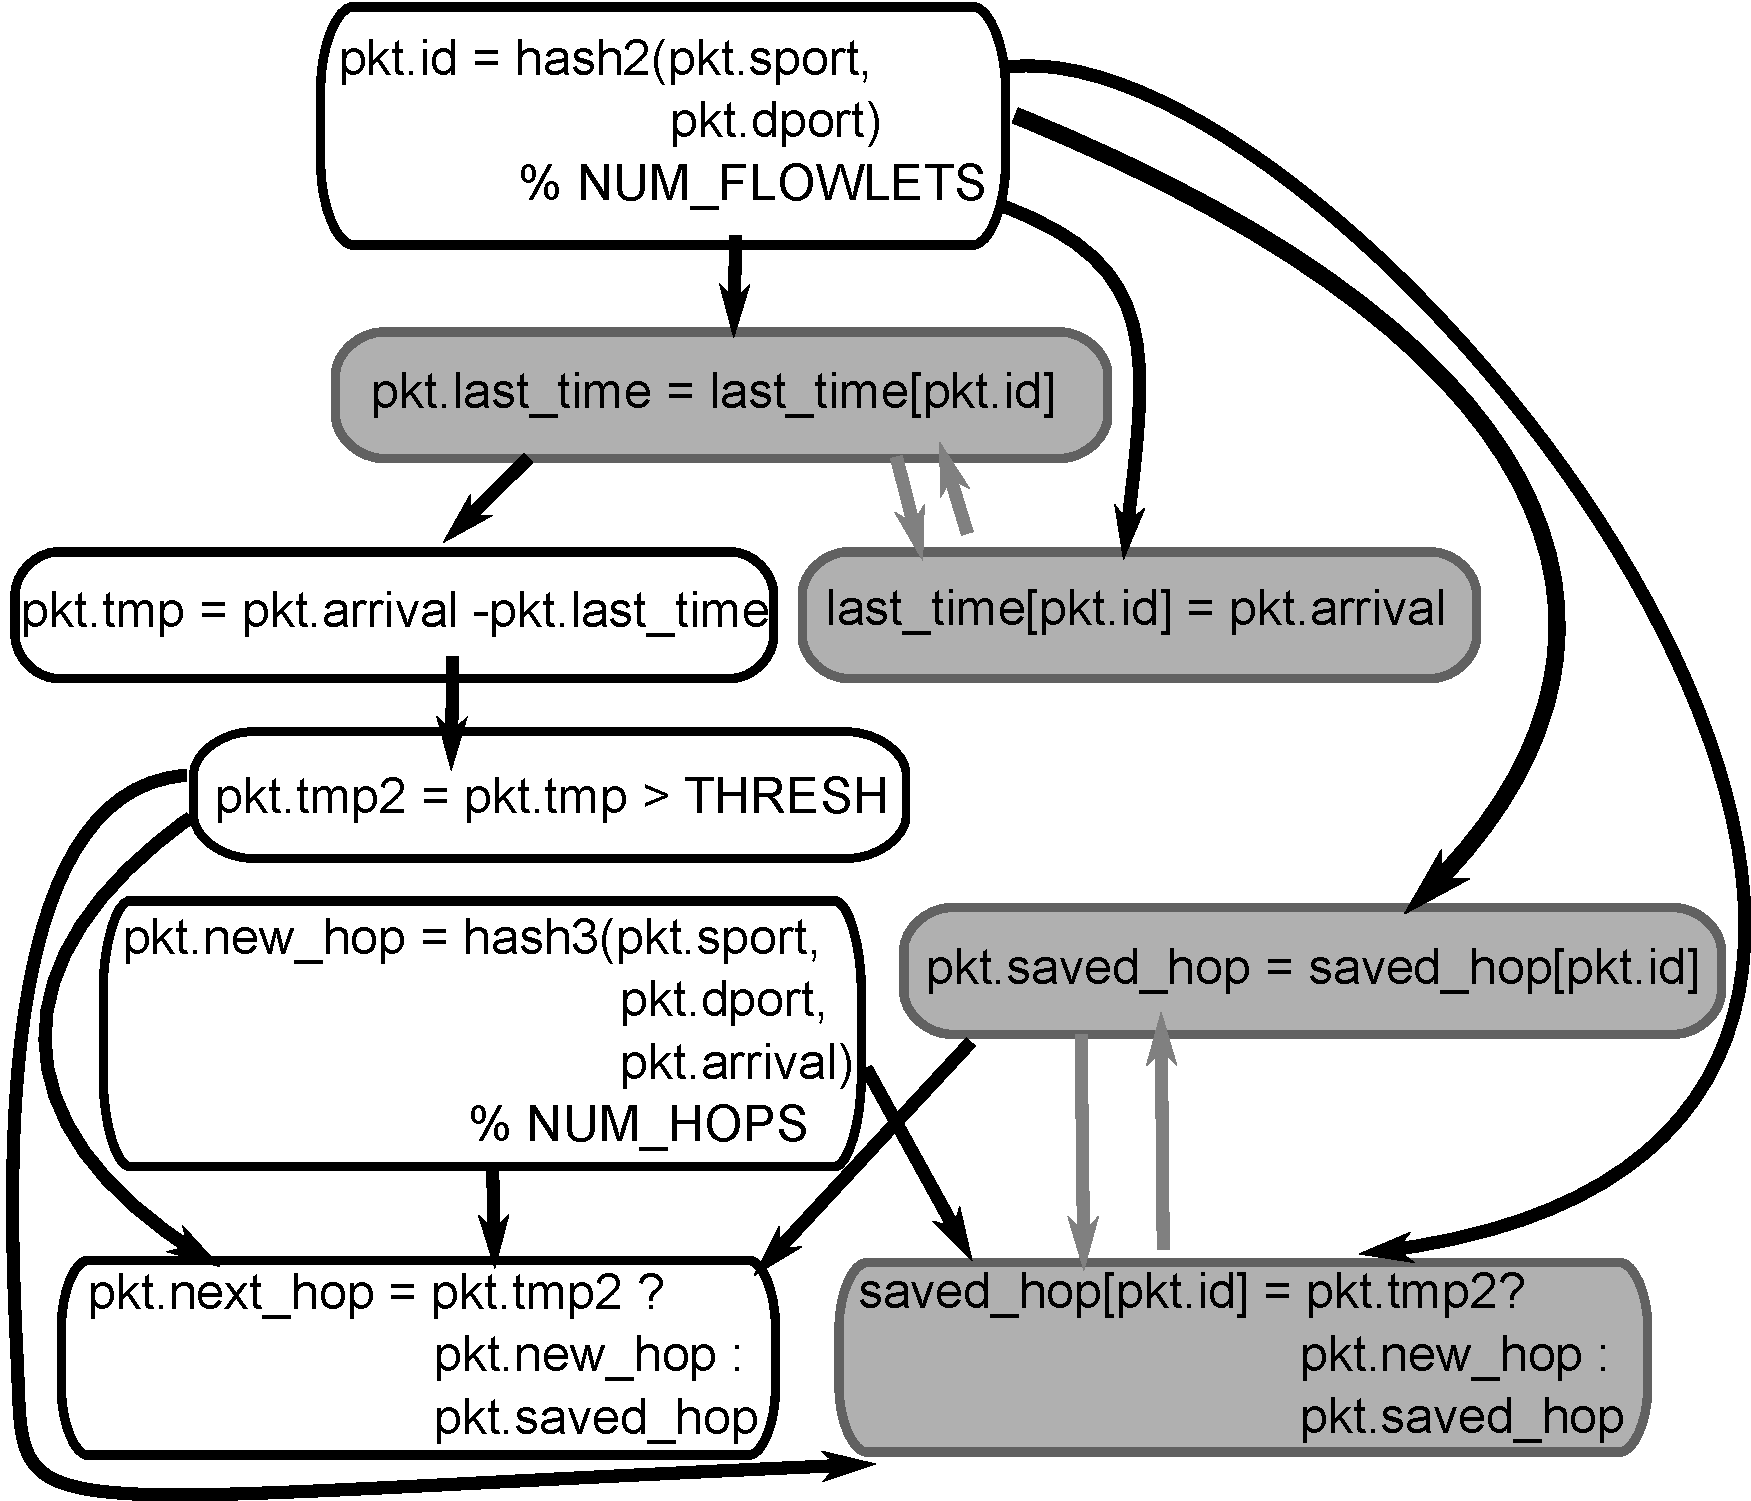
\includegraphics[width=0.98\columnwidth]{domino_deps.pdf}
  \caption{Stateless dependencies in black, stateful in gray.}
  \label{fig:partitioning_before}
\end{subfigure}
\textbf{$\Longrightarrow$ }
\begin{subfigure}{\columnwidth}
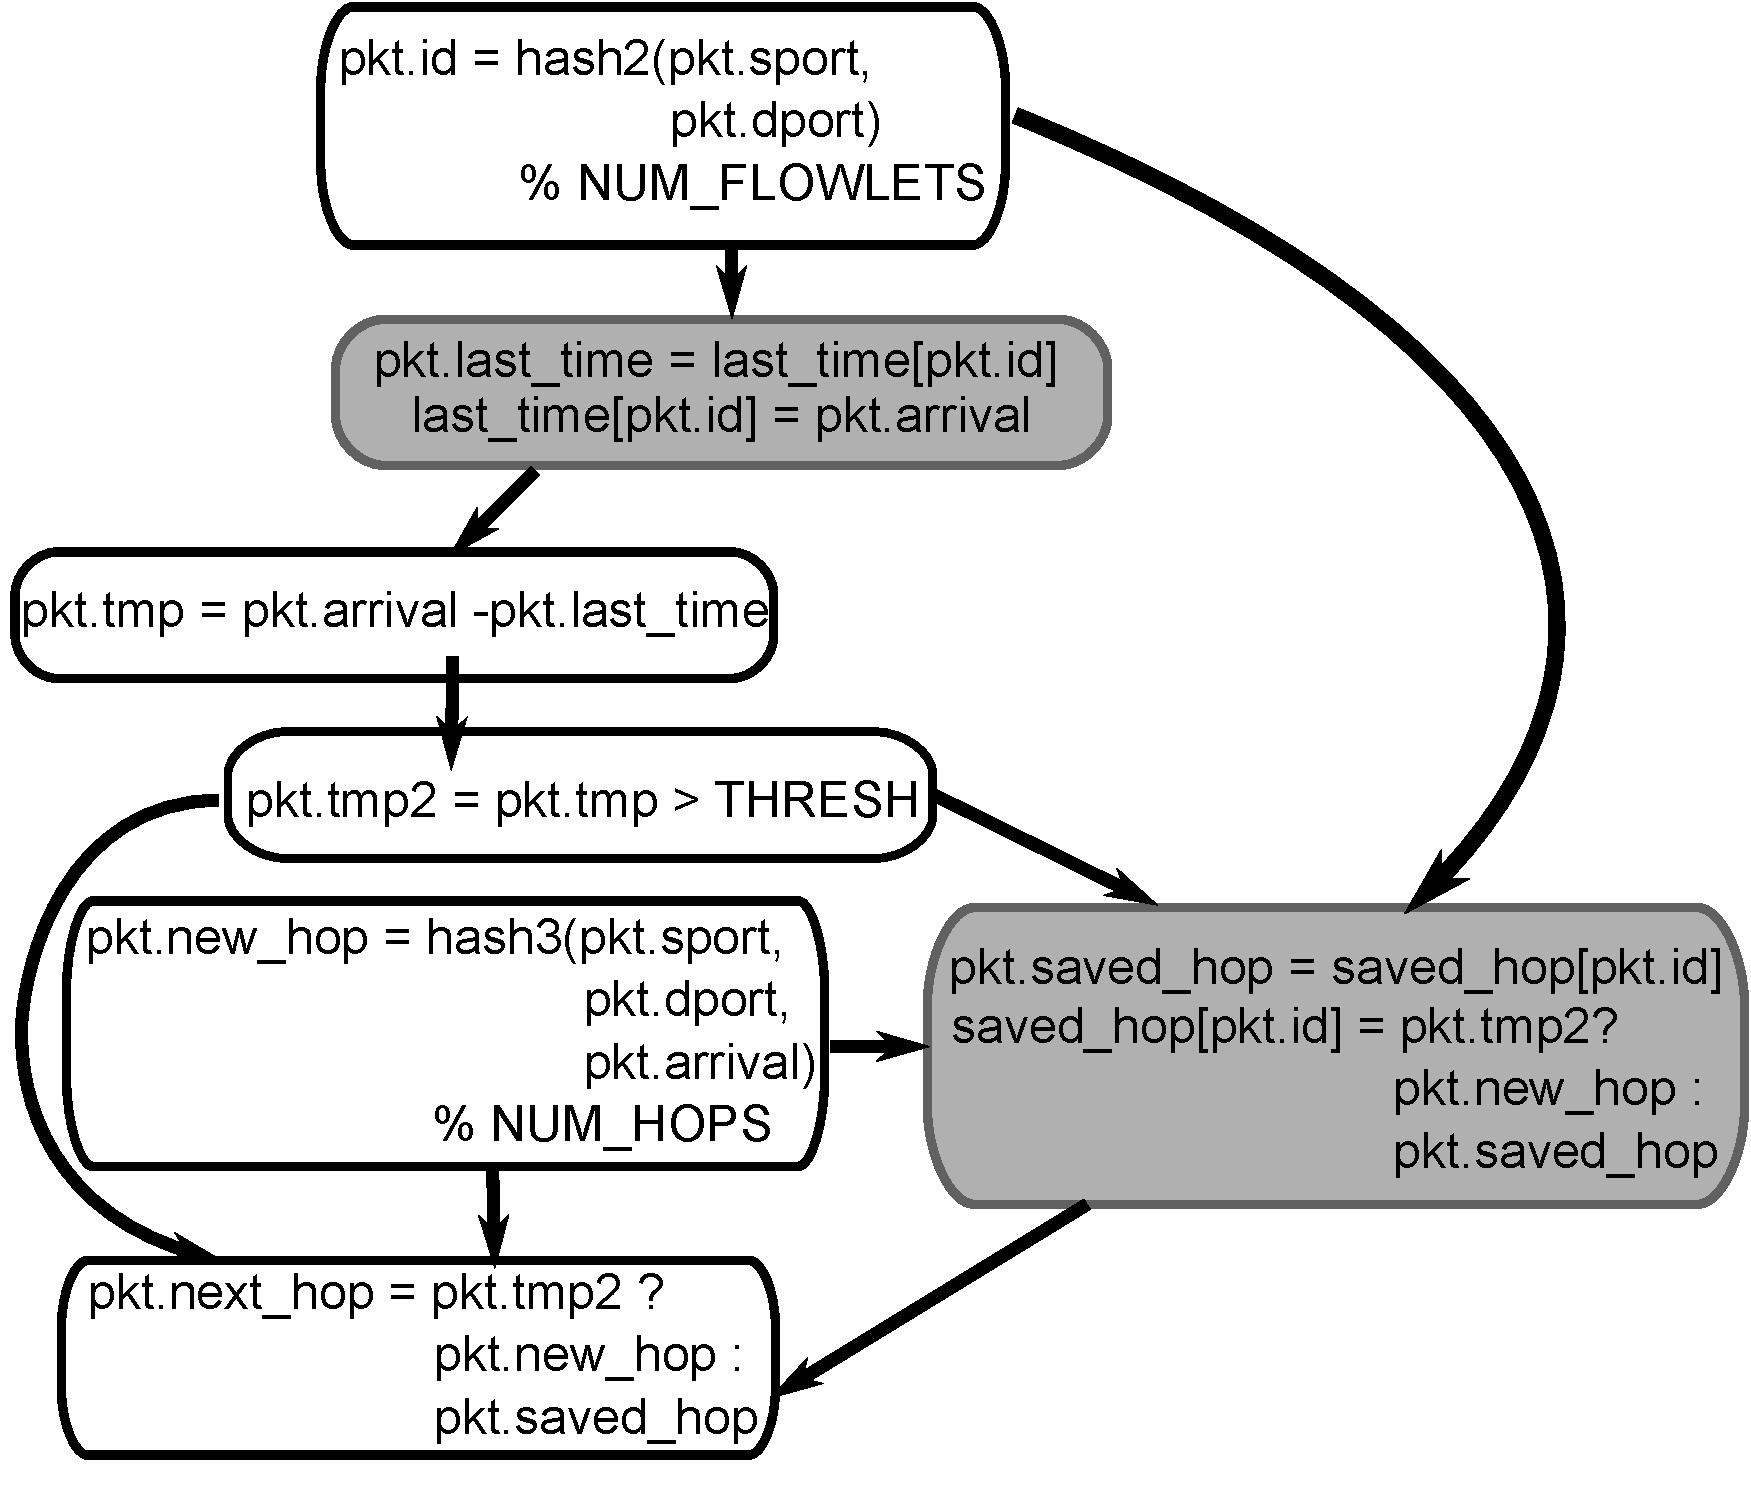
\includegraphics[width=0.98\columnwidth]{domino_scc.pdf}
\caption{DAG after condensing SCCs.}
\label{fig:partitioning_after}
\end{subfigure}
\caption{Dependency graphs before and after condensing strongly connected components}
\label{fig:pipelining}
\end{figure*}




\subsection{Code generation}
\label{ss:code_gen}

To determine if a codelet pipeline can be compiled to a \absmachine machine, we
consider two constraints specified by any \absmachine machine
(\S\ref{s:atomConstraints}).  Resource limits specify the number of atoms in a
stage (pipeline width) and number of stages (pipeline depth), while
computational limits specify the atom templates provided by a \absmachine
machine.

\medskip
\noindent
\textbf{Resource limits.} To handle resource limits, we scan each pipeline
stage in the codelet pipeline starting from the first to check for pipeline
width violations. If we violate the pipeline width, we insert as many new
stages as required and spread codelets evenly across these stages.  We continue
until the number of codelets in all stages is under the pipeline width,
rejecting the program if we exceed the pipeline depth.

\medskip
\noindent
\textbf{Computational limits.} Next, we determine if each codelet in the pipeline
can be mapped to atoms provided by the \absmachine machine. In general,
codelets have multiple three-address code statements that need to execute
atomically. For instance, updating the state variable \texttt{saved\_hop} in
Figure~\ref{fig:flowlet_pipeline} requires a read followed by a conditional
write.  It is not apparent whether such codelets can be mapped to an available
atom. We develop a new technique to determine the implementability of a codelet,
given an atom template.

Each atom template has a set of configuration parameters, where the parameters
determine the atom's behavior.  For instance, Figure~\ref{fig:alu_diag} shows
an atom that can perform stateful addition or subtraction, depending on the
configuration parameters {\tt choice} and {\tt constant}.  Each codelet can be
viewed as a functional specification of the atom.  With that in mind, the
mapping problem is equivalent to searching for values of the atom's configuration
parameters that result in the atom implementing the codelet.

We use the SKETCH program synthesizer~\cite{sketch_asplos} for this purpose, as
the atom templates can be easily expressed using SKETCH. SKETCH also
provides efficient search algorithms and has been used for similar purposes in
other domains~\cite{lifejoin, qbs}. As an
illustration, assume we want to map the codelet {\tt x=x+1} to the atom
template shown in Figure~\ref{fig:alu_in_sketch}. SKETCH will search for
possible parameter values so that the resulting atom is functionally identical
to the codelet, for all possible input values of {\tt x} up to a certain bound. 
In this case, SKETCH
finds the solution with {\tt choice=0} and {\tt constant=1}.  In contrast, if
the specification is the codelet {\tt x=x*x}, SKETCH will return
an error as no parameters exist.

Using program synthesis for code generation frees the compiler developer from implementing
custom code generators for different \absmachine machines.
Instead, the
compiler developer only has to express the \absmachine machine's
atom templates using SKETCH, and the SKETCH synthesizer automatically maps
codelets to atoms.

%%To minimize search time, the range
%%of possible inputs and parameter values need to be specified in the template
%%(e.g., all 8 bit integers), and our experiments show that the search finishes
%%quickly, taking 10 secs at most.

\subsection{Related compiler techniques}
\label{ss:related_compiler}
Table~\ref{tab:prior_compiler} shows the relationship between \pktlanguage's
compilation techniques and prior work. The use of Strongly Connected Components
(SCCs) is inspired by software pipelining for VLIW
architectures~\cite{software_pipelining}. The size of the largest SCC affects
the {\em maximum throughput} of the pipelined loop in software pipelining. For
\pktlanguage, it affects the {\em circuit area} of the atom required to run a
program at line rate. \pktlanguage trades off an increase in space for
line-rate performance.

Program synthesis was used for code generation in
Chlorophyll~\cite{chlorophyll}.  Code generation for \pktlanguage also shares
similar goals to technology mapping~\cite{micheli} and
instruction selection~\cite{dragonbook}.  However, prior work maps a code sequence
to \textit{multiple} instructions/tiles, using heuristics to minimize
instruction count. Domino's problem is simpler: we map each codelet to a single
atom using SKETCH.  The simpler problem allows a non-heuristic solution: if
there is any way to map the codelet to an atom, SKETCH will find it.

Branch removal resembles If-Conversion~\cite{if_conversion}, a
technique used in vectorizing compilers. This procedure is easier in Domino
because there is no backward control transfer ({\tt goto}, {\tt break},
{\tt continue}).

\begin{table}[!t]
  \centering
  \begin{small}
    \begin{tabular}{|p{0.2\textwidth}|p{0.2\textwidth}|p{0.4\textwidth}|}
  \hline
  Technique & Prior Work & Differences \\
  \hline
  Conversion to straight-line code & If-Conversion~\cite{if_conversion} & No backward control flow (gotos, break, continue) \\
  \hline
  SSA & Cytron et al.~\cite{ssa} & SSA runs on straight-line code with no branches \\
  \hline
  Strongly Connected Components & Lam~\cite{software_pipelining} & Scheduling in space vs. time \\
  \hline
  Code generation using program synthesis & Chlorophyll~\cite{chlorophyll}, technology mapping~\cite{micheli}, instruction selection~\cite{dragonbook} & Optimal vs. best-effort mapping, One-to-one mapping vs. one-to-many mapping \\
  \hline
  \end{tabular}
  \end{small}
  \caption{Domino's compiler in relation to prior work}
  \label{tab:prior_compiler}
\end{table}

\section{Evaluation}
\label{s:eval}

\begin{table}[!t]
\begin{small}
  \begin{tabular}{|p{0.3\columnwidth}|p{0.6\columnwidth}|p{0.06\columnwidth}|p{0.06\columnwidth}|}
\hline
Algorithm & Stateful operations & LOC & P4 LOC\\
\hline
Bloom filter (3 hash functions) & Test/Set membership bit on every packet. & 29 & 104 \\
\hline
Heavy Hitters~\cite{opensketch} (3 hash functions) & Increment count-min sketch~\cite{cormode} on every packet. & 35 & 192 \\
\hline
Flowlets~\cite{flowlets} & Update saved next hop if flowlet threshold is exceeded.& 37 & 107 \\
\hline
RCP~\cite{rcp} & Accumulate RTT sum if RTT is under maximum allowable RTT. & 23 & 75 \\
\hline
Sampled NetFlow~\cite{sampled_nflow} & Sample a packet if packet count reaches N. Reset count to 0 when it reaches N. & 18 & 70 \\
\hline
HULL~\cite{hull} & Update counter for virtual queue. & 26 & 95 \\
\hline
Adaptive Virtual Queue~\cite{avq} & Update virtual queue size and virtual capacity. & 36 & 147 \\
\hline
Priority computation for weighted fair queueing (Chapter~\ref{chap:pifo}) & Compute packet's virtual start time using finish time of last packet in that flow. & 29 & 87 \\
\hline
DNS TTL change tracking~\cite{dns_change} & Track number of changes in announced TTL for each domain. & 27 & 119 \\
\hline
CONGA~\cite{conga} & Update best path's utilization/id if we see a better path. Update best path utilization alone if it changes.  & 32 & 89\\
\hline
%trTCM~\cite{trTCM} & Update token counts for each token bucket & Doesn't map & 7, 3 & Either \\
%\hline
CoDel~\cite{codel} & Update whether we are marking or not, time for next mark, number of marks so far, and time at which minimum queueing delay will exceed target. & 57 & 271\\
\hline
\end{tabular}
\end{small}
\caption{Data-plane algorithms}
\label{tab:algorithms}
\end{table}


We evaluate \pktlanguage's expressiveness by using it to program several
data-plane algorithms (Table~\ref{tab:algorithms}), and comparing it to writing
them in P4~(\S\ref{ss:expressiveness}). To validate that these
algorithms can run at line rate, we design a concrete set of \absmachine
machines (Table~\ref{tab:templates}) as compiler targets for
\pktlanguage~(\S\ref{ss:targets}).  We estimate that these machines are
feasible in hardware because their atoms incur modest chip area overhead.  We
use the \pktlanguage compiler to compile the algorithms in
Table~\ref{tab:algorithms} to the targets in
Table~\ref{tab:templates}~(\S\ref{domino_ss:compiler}).  We conclude with some
lessons for programmable router design~(\S\ref{ss:lessons}).

\subsection{Expressiveness}
\label{ss:expressiveness}

We program several data-plane algorithms (Table~\ref{tab:algorithms}) using
\pktlanguage. These algorithms encompass data-plane traffic engineering,
in-network congestion control, active queue management, network security, and
measurement. We also used \pktlanguage to express the priority computation for
programming scheduling using push-in first-out queues, as described in greater
detail in Chapter~\ref{chap:pifo}.

In all these cases, the algorithms are already available as blocks of
imperative code from online sources; translating them to \pktlanguage syntax
was straightforward. In contrast, expressing any of them in P4\footnote{We are
referring to P4 at the time the Domino paper was published. As we describe in
\S\ref{s:impact}, many of Domino's ideas (including packet transactions) are
part of the latest version of P4.}
requires manually teasing out portions of the algorithm that can reside in
independent match-action tables and then chaining these tables together.

Of the algorithms in Table~\ref{tab:algorithms}, only flowlet switching has a
publicly available P4 implementation~\cite{p4_flowlet} that we can compare
against. This implementation requires 231 lines of uncommented P4, compared to
only 37 lines of \pktlanguage code in Figure~\ref{fig:flowlet_code}. Not only
that, using P4 also requires the programmer to manually specify tables, the
actions within tables, and how tables are chained---all to implement a single
data-plane algorithm. The \pktlanguage compiler automates this process; to
demonstrate this, we developed a backend for \pktlanguage that generates the
equivalent P4 code. We list the number of lines of code for these
auto-generated P4 programs in Table~\ref{tab:algorithms}.
%%
%%Data-plane algorithms on software platforms today (NPUs, Click, the Linux qdisc
%%subsystem~\cite{qdisc})  are programmed in languages resembling
%%\pktlanguage---hence we are confident that the \pktlanguage syntax is already
%%familiar to network engineers.
%%
\subsection{Compiler targets}
\label{ss:targets}

We design a set of compiler targets for \pktlanguage based on the \absmachine
machine model (\S\ref{s:absmachine}). First, we describe how to assess the
feasibility of atoms: whether they can run at a 1 GHz clock frequency, and what
area overhead they incur in silicon. Next, we discuss the design of stateless
and stateful atoms separately. Finally, we discuss how these stateless and
stateful atoms are combined together in our compiler targets.

\Para{Atom feasibility.}
We synthesize a digital circuit corresponding to an atom template by writing
the atom template in Verilog, and using the Synopsys Design
Compiler~\cite{synopsys_dc} to compile the Verilog code. The Design Compiler
checks if the resulting circuit meets timing at 1 GHz in a 32-nm standard-cell
library, and outputs its gate area. We use this gate area, along with the area
of a 200 \si{\milli\metre\squared} baseline router chip~\cite{gibb_parsing},
to estimate the area overhead for provisioning a \absmachine machine with
multiple instances of this atom.

% (a library of primitive gates designed using a
%transistor with a feature size of 32 nm)

\Para{Designing stateless atoms.}
Stateless atoms are easier to design because arbitrary stateless operations can
be broken up into multiple pipeline stages without violating
atomicity~(\S\ref{ss:atoms}). We design a stateless atom that can support
simple arithmetic (add, subtract, left shift, right shift), logical (and, or,
xor), relational ({\tt >=}, {\tt <=}, {\tt ==}, {\tt !=}), and conditional
instructions (C's ``{\tt ?}'' operator) on a pair of packet fields. Any packet
field can also be substituted with a constant operand. This stateless atom
meets timing at 1 GHz and occupies an area of 1384 \si{\micro\meter\squared}
(Table~\ref{tab:templates}).

\Para{Designing stateful atoms.}
The choice of stateful atoms determines the algorithms a line-rate router can
support. A more complex stateful atom can support more data-plane algorithms,
but may not meet timing at 1 GHz and occupies more area. To illustrate this
effect, we design a containment hierarchy (Table~\ref{tab:templates}) of
stateful atoms, where each atom can express all stateful operations that its
predecessor can.  These atoms start out with the simplest stateful capability:
the ability to read or write state alone.  They then move on to the ability to
read, add, and write back state atomically (RAW), a predicated version of the
same (PRAW), and so on. When synthesized to a 32-nm standard-cell library, all
our stateful atoms meet timing at 1 GHz.  However, the atom's area and minimum
end-to-end propagation delay increases with the atom's
complexity~(Table~\ref{tab:templates}).

\Para{The compiler targets.}
We design seven \absmachine machines as compiler targets. A single \absmachine
machine has 600 atoms.
\begin{CompactEnumerate}
\item 300 are stateless atoms of the single stateless atom type from
Table~\ref{tab:templates}.
\item 300 are stateful atoms of one of the seven stateful atom types from
Table~\ref{tab:templates} (Read/Write through Pairs).
\end{CompactEnumerate}
These 300 stateless and stateful atoms are laid out physically as 10 stateless
and stateful atoms per pipeline stage and 30 pipeline stages. While the number
300 and the pipeline layout are arbitrary, they are sufficient for all examples
in Table~\ref{tab:algorithms}, and incur modest area overhead as we show next. In
the future, we anticipate these numbers being decided empirically based on what
algorithms are most frequently run on such platforms.

We estimate the area overhead of these seven targets relative to a 200
\si{\milli\metre\squared} chip~\cite{gibb_parsing}, which is at the lower end
of chip sizes today. For this, we multiply the individual atom areas from
Table~\ref{tab:templates} by 300 for both the stateless and stateful atoms. For
300 atoms, the area overhead is 0.2 \% for the stateless atom and 0.9 \% for
the Pairs atom, the largest among our stateful atoms.  The area overhead
combining both stateless and stateful atoms for all our targets is at most
1.1\%---a modest price for the programmability it provides.
%TODO: Add mux area? I think it's too detailed to include here.
\begin{table}[!t]
  \centering
  \begin{small}
  \begin{tabular}{|p{0.26\textwidth}|p{0.36\textwidth}|p{0.08\textwidth}|p{0.04\textwidth}|}
    \hline
    Atom & Description & Area (\si{\micro\metre\squared}) at 1 GHz & Min. delay (ps) \\
    \hline
    Stateless & Arithmetic, logic, relational, and conditional operations on packet/constant operands & 1384 & 387 \\
    \hline
    Read/Write & Read/Write packet field/constant into single state variable. & 250 & 176 \\
    \hline
    ReadAddWrite (RAW) & Add packet field/constant to state variable (OR) Write packet field/constant into state variable. & 431 & 316 \\
    \hline
    Predicated ReadAddWrite (PRAW) & Execute RAW on state variable only if a predicate is true, else leave unchanged. & 791 & 393 \\
    \hline
    IfElse ReadAddWrite (IfElseRAW) & Two separate RAWs: one each for when a predicate is true or false. & 985 & 392 \\
    \hline
    Subtract (Sub) & Same as IfElseRAW, but also allow subtracting a packet field/constant. & 1522 & 409 \\
    \hline
    Nested Ifs (Nested) & Same as Sub, but with an additional level of nesting that provides 4-way predication. & 3597 & 580 \\
    \hline
    Paired updates (Pairs) & Same as Nested, but allow updates to a pair of state variables, where predicates can use the earlier values of both state variables. & 5997 & 606 \\
    \hline
  \end{tabular}
  \end{small}
  \caption{Atom areas and minimum critical-path delays in a 32-nm standard-cell
library.  All atoms meet timing at 1 GHz. Each of the seven compiler targets
contains 300 instances of one of the seven stateful atoms (Read/Write to Pairs)
and 300 instances of the single stateless atom.}
  \label{tab:templates}
\end{table}

\subsection{Compiling \pktlanguage programs to \absmachine machines}
\label{domino_ss:compiler}
We now consider every target from Table~\ref{tab:templates} and every
data-plane algorithm from Table~\ref{tab:algorithms} to determine if the algorithm
can run at the line rate of a particular \absmachine machine. Because every
target is uniquely identified by its stateful atom type, we use the name of the
stateful atom to refer to the target itself.

We say an algorithm can run at line rate on a \absmachine machine if every
codelet within the data-plane algorithm can be mapped (\S\ref{ss:code_gen}) to
either the stateful or stateless atoms provided by the \absmachine machine.
Because our stateful atoms are arranged in a containment hierarchy, we list the
\textit{most expressive} stateful atom/target required for each data-plane
algorithm in Table~\ref{tab:algo_atoms}.
%TODO: Need to add a column about state requirements and guards 
\begin{table}[!t]
\begin{small}
  \begin{tabular}{|p{0.3\columnwidth}|p{0.1\columnwidth}|p{0.05\columnwidth}|p{0.05\columnwidth}|p{0.08\columnwidth}|}
\hline
Algorithm & Most expressive atom required & Stages & Max. atoms/stage & Ingress or Egress Pipeline?\\
\hline
Bloom filter (3 hash functions) & Read/Write & 4 & 3 & Either\\
\hline
Heavy Hitters~\cite{opensketch} (3 hash functions) & RAW & 10 & 9 & Either\\
\hline
Flowlets~\cite{flowlets} & PRAW & 6 & 2 & Ingress\\
\hline
RCP~\cite{rcp} & PRAW & 3 & 3 & Egress\\
\hline
Sampled NetFlow~\cite{sampled_nflow} & IfElseRAW & 4 & 2 & Either\\
\hline
HULL~\cite{hull} & Sub & 7 & 1 & Egress\\
\hline
Adaptive Virtual Queue~\cite{avq} & Nested & 7 & 3 & Ingress\\
\hline
Priority computation for weighted fair queueing (Chapter~\ref{chap:pifo}) & Nested & 4 & 2 & Ingress\\
\hline
DNS TTL change tracking~\cite{dns_change} & Nested & 6 & 3 & Ingress\\
\hline
CONGA~\cite{conga} & Pairs & 4 & 2 & Ingress\\
\hline
%trTCM~\cite{trTCM} & Update token counts for each token bucket & Doesn't map & 7, 3 & Either \\
%\hline
CoDel~\cite{codel} & Doesn't map & 15 & 3 & Egress\\
\hline
\end{tabular}
\end{small}
\caption{Mapping Domino algorithms to atoms}
\label{tab:algo_atoms}
\end{table}


As Table~\ref{tab:algo_atoms} shows, the choice of stateful atom determines what
algorithms can run on a router. For instance, with only the ability to read or
write state, only the Bloom Filter algorithm can run at line rate, because it
only requires the ability to test and set membership bits.  Adding the ability
to increment state (the RAW atom) permits Heavy Hitters to run at line rate,
because it employs a count-min sketch that is incremented on each packet.

\subsection{Lessons for programmable routers}
\label{ss:lessons}

\Para{Atoms that allow modifications to a single state variable support many
algorithms.} The algorithms from Bloom Filter through DNS TTL Change Tracking
in Table~\ref{tab:algo_atoms} can run at line rate using the Nested Ifs atom that
modifies a single state variable.

\Para{But, some algorithms modify a pair of state variables atomically.}
An example is CONGA; we reproduce CONGA's relevant code snippet below:
\begin{verbatim}
  if (p.util < best_path_util[p.src]) {
    best_path_util[p.src] = p.util;
    best_path[p.src] = p.path_id;
  } else if (p.path_id == best_path[p.src]) {
    best_path_util[p.src] = p.util;
  }
\end{verbatim}
Here, \texttt{best\_path} (the path id of the best path for a particular
destination) is updated conditioned on \texttt{best\_path\_util} (the
utilization of the best path to that destination)\footnote{{\tt p.src} is the
address of the host originating this message, and hence the destination for the
host receiving it and executing CONGA.} and vice versa. These two state
variables cannot be separated into different stages and still guarantee a
packet transaction's semantics because they are mutually dependent on each
other.  The Pairs atom, where the update to a state variable is conditioned on
a predicate of a pair of state variables, allows CONGA to run at line rate.

\Para{There will always be algorithms that cannot run at a target's line rate.}
While the targets and their atoms in Table~\ref{tab:templates} are sufficient
for several data-plane algorithms, there are algorithms that they cannot run at
line rate.  An example is CoDel, which cannot be implemented because it
requires a square root operation that is not provided by any of our targets.
One possibility is a look-up table abstraction that allows us to approximate
such mathematical functions. However, regardless of what set of atoms we design
for a particular target, there will always be algorithms that cannot run at
line rate.

%%This is because the set of computations that can be
%%expressed by an atom (or a finite pipeline of atoms) are finite because these
%%computations all need to finish within a ns, while the set of algorithms is
%%infinite.

\begin{table}[!t]
  \centering
  \begin{small}
    \begin{tabular}{|p{0.18\textwidth}|p{0.61\textwidth}|p{0.06\textwidth}|}
  \hline
  Atom & Circuit & Min. delay (ps) \\
  \hline
  Read/Write & \centering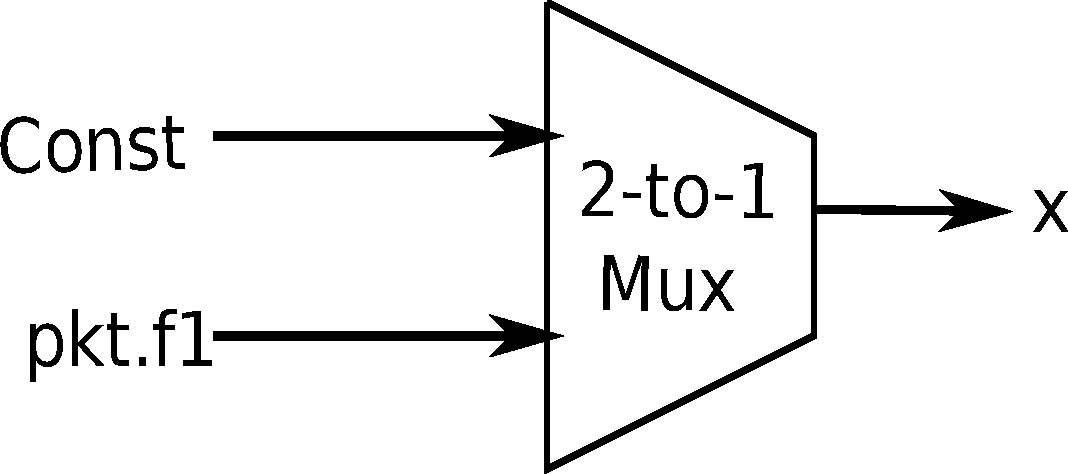
\includegraphics[width=0.4\textwidth]{domino_rw.pdf} & 176 \\
  \hline
  ReadAddWrite (RAW) & \centering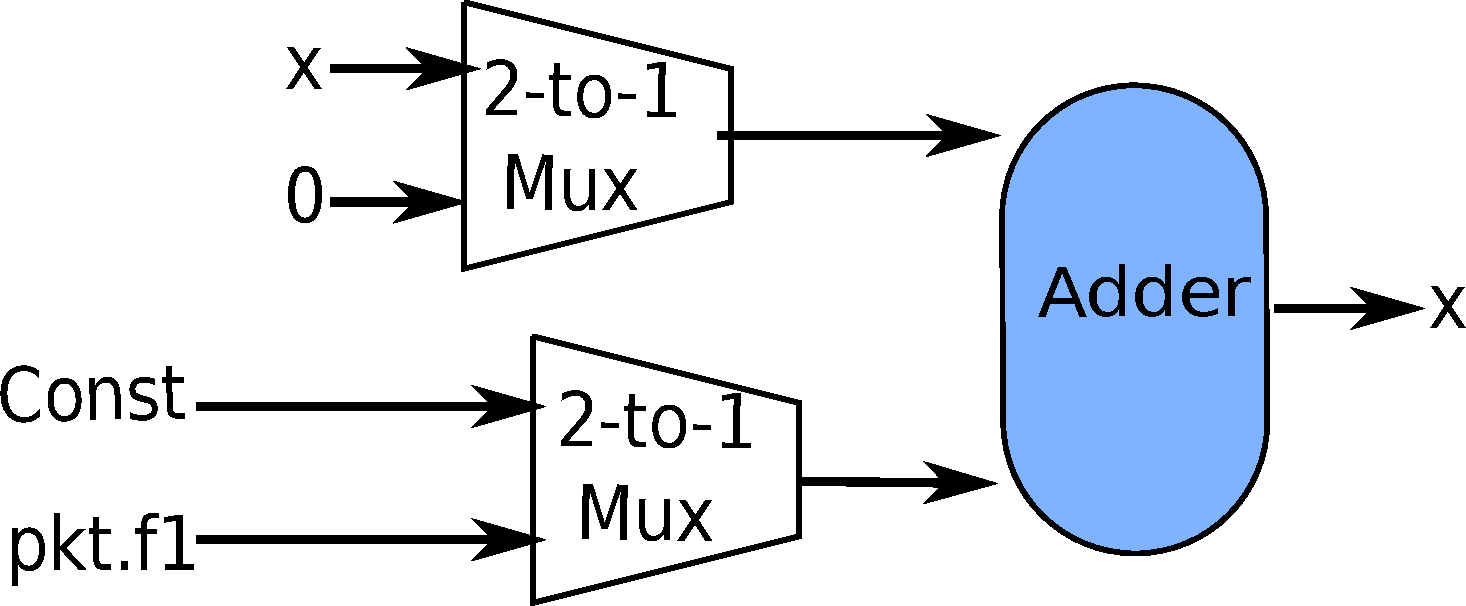
\includegraphics[width=0.5\textwidth]{domino_raw.pdf} & 316\\
  \hline
  \pbox{0.1\textwidth}
  {Predicated\\
  ReadAddWrite (PRAW)} & \centering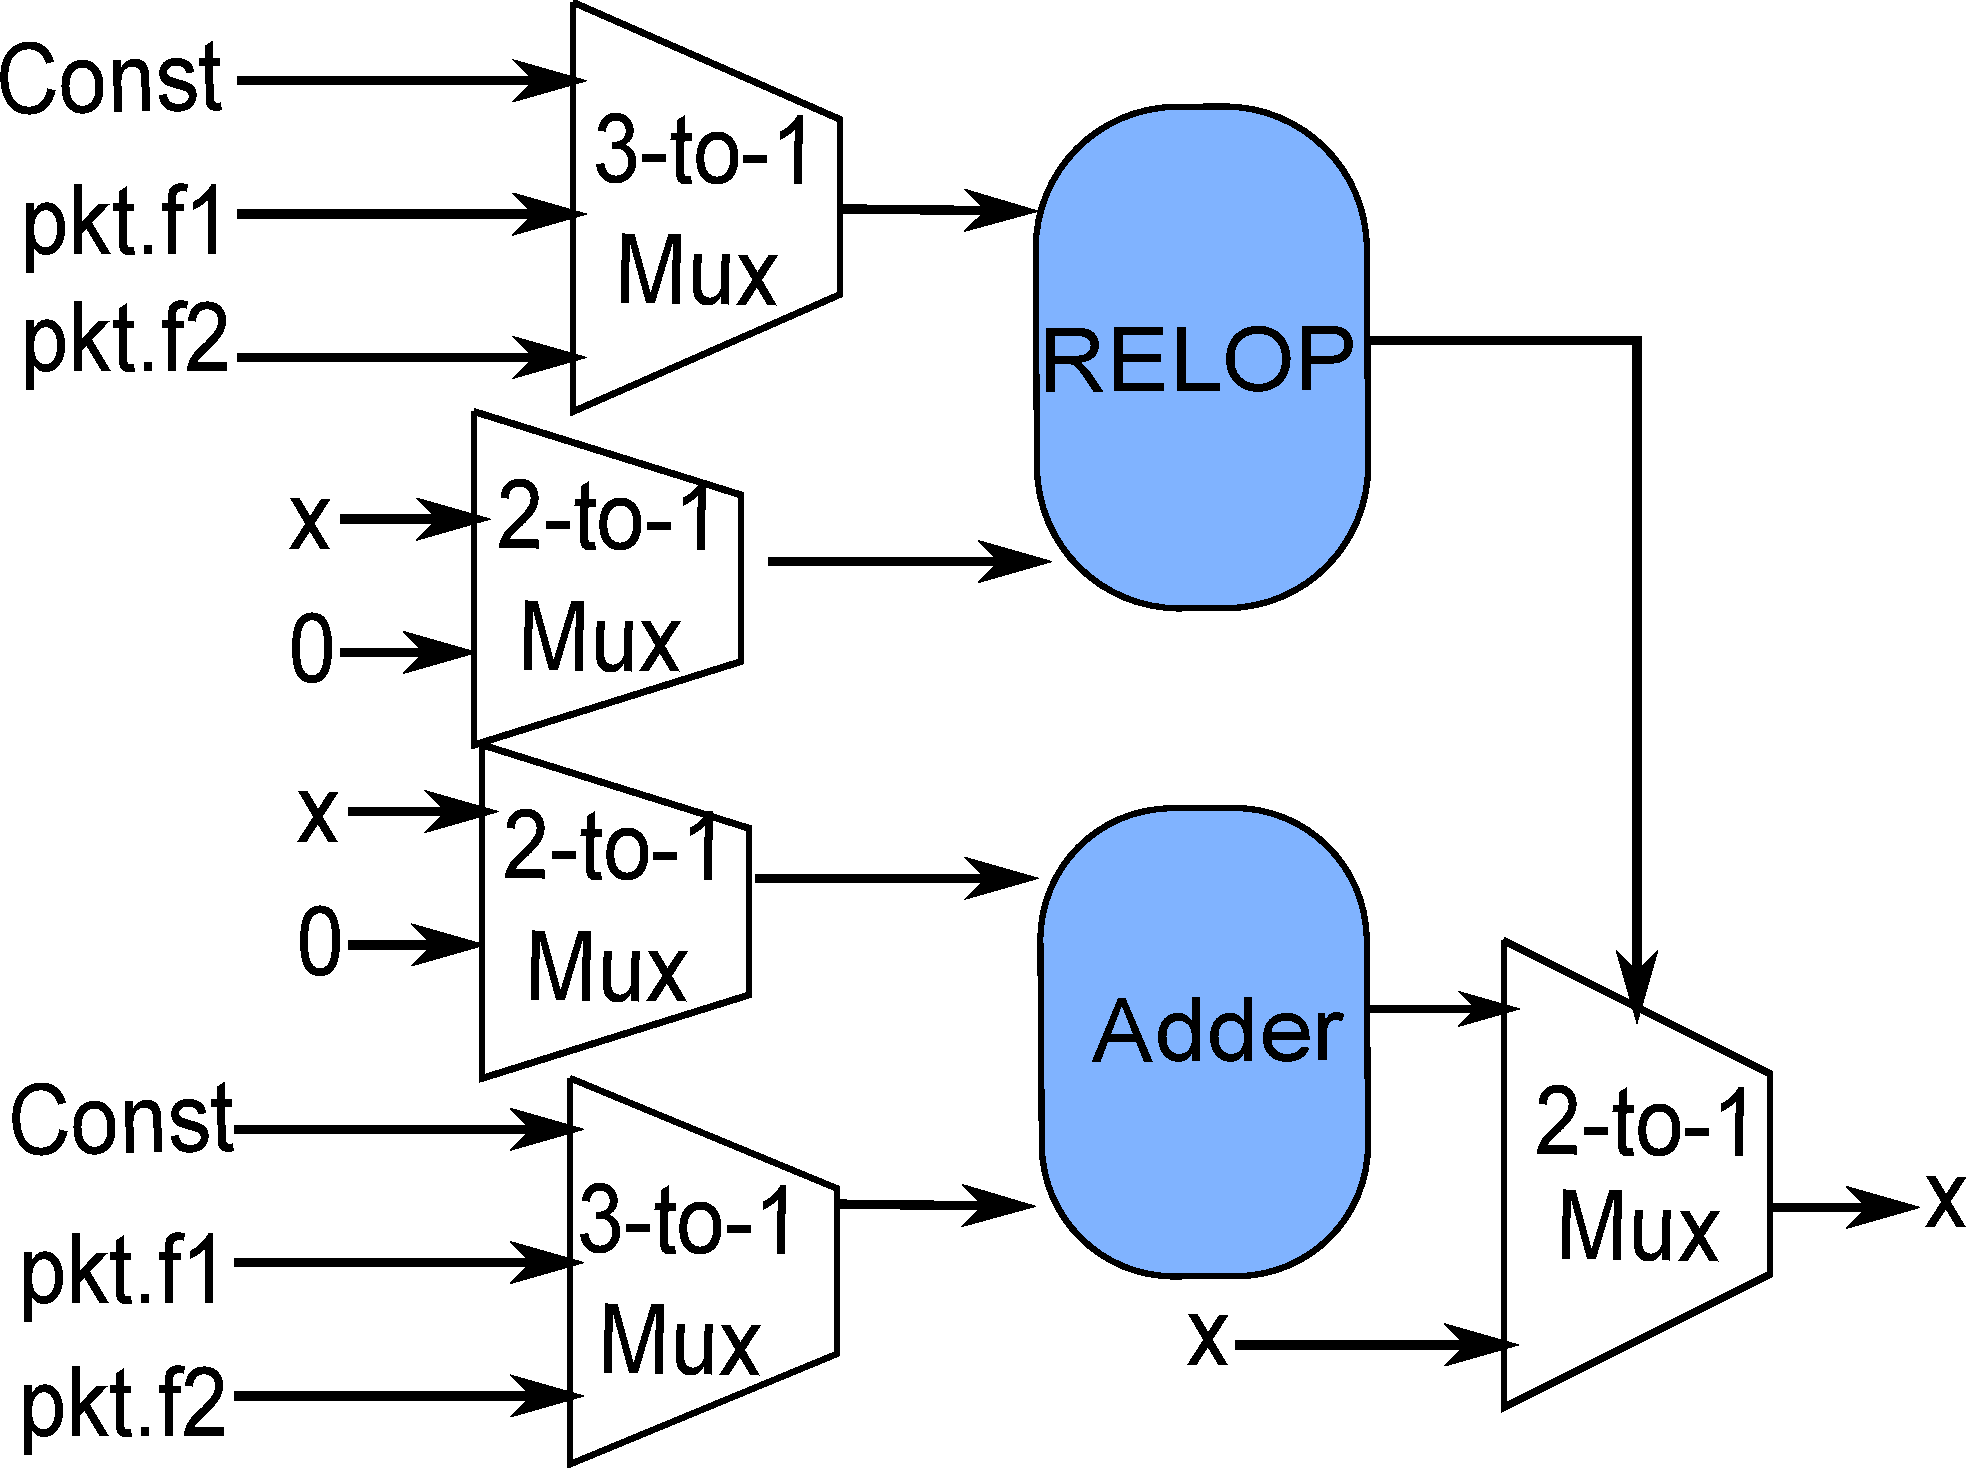
\includegraphics[width=0.6\textwidth]{domino_pred_raw.pdf}  & 393 \\
  \hline
  \end{tabular}
\end{small}
\caption{An atom's minimum critical-path delay (\ie, the lowest possible
critical-path delay on a particular standard cell library) increases with
circuit depth.  Mux is a multiplexer. RELOP is a relational operation (>, <,
==, !=). {\tt x} is a state variable. {\tt pkt.f1} and {\tt pkt.f2} are packet
fields. {\tt Const} is a constant operand.}
\label{tab:circuits}
\end{table}



\Para{Atom design is constrained by timing, not area.} Atoms are affected by
two factors: their area and their timing, \ie the delay on the critical path of
the atom's combinational circuit. For the few hundred atoms that we require,
atom area is insignificant (< 2\%) relative to chip area.  Further, even for
future atoms that are larger, area may be controlled by provisioning fewer atom
instances.

However, atom timing is critical. Table~\ref{tab:templates} shows a 3.4
$\times$ range in minimum critical-path delay (\ie the lowest achievable
critical path on a particular standard-cell library) between the simplest and
the most complex atoms.  This increase can be explained by looking at the
simplified circuit diagrams for the first three atoms
(Table~\ref{tab:circuits}), which show an increase in circuit depth with atom
complexity.

%TODO: critical-path delay or min. critical-path delay. Decide.
% This is really really muddled.
Because the clock frequency of a circuit is at least as small as the reciprocal
of the critical-path delay, a more complex atom results in a lower clock
frequency and a lower line rate. Although all our atoms have a minimum
critical-path delay under 1 ns (1 GHz), it is conceivable that they can be
extended with functionality that causes the atom to violate timing at 1 GHz.

In summary, for a router designer, the critical path of atoms is the most
important metric to optimize. The most programmable line-rate routers will have
the highest density of useful stateful functionality squeezed into a critical
path budget of 1 clock cycle.

\Para{Compilers can be used to design instruction sets.} Designing an
instruction set for a programmable substrate is a chicken-and-egg problem: the
choice of instructions determines which algorithms can execute on that target,
while the choice of algorithms dictates what instructions are required in the
target. Indeed, other programmable substrates (\eg graphics processors and
digital signal processors) go through an iterative process to design a good
instruction set.

 A compiler can aid this process. To show how, we describe how we designed the
stateful atoms in Table~\ref{tab:templates}. We pick a data-plane algorithm and
partially execute the \pktlanguage compiler to generate a codelet pipeline.  We
then inspect the stateful codelets, and create an atom that expresses all the
computations required by the stateful codelets. We verify that this atom can
indeed express all these computations by fully executing the compiler on the
data-plane algorithm with that atom as the target. We then move on to the next
algorithm, and check if the same atom suffices. If not, we repeatedly extend
our atom through a process of trial-and-error to capture more computations, all
the while using the compiler to verify our intuitions on extending atoms. In
the process, we generate a hierarchy of atoms, each of which works for a subset
of algorithms.

Our atom design process is manual and ad hoc at this point, but it already
shows how  a compiler can aid in instruction-set design for programmable
routers. Using the same iterative approach involving a compiler, we anticipate
the atoms in \absmachine machines evolving as data-plane algorithms demand more
of the hardware.

%%\textbf{Compilation time:}
%%Compilation time is dominated by SKETCH's search procedure.  To speed up the
%%search, we limit SKETCH to search for constants (\eg for addition) of size up
%%to 5 bits, given that the constants seen within stateful codelets in our
%%algorithms are small. Our longest compilation time is 10 seconds when CoDel
%%doesn't map to a \absmachine machine with the Pairs atom because SKETCH has to
%%rule out every configuration in its search space.  This time will increase if
%%we increase the bit width of constants that SKETCH has to search; however,
%%because the data-plane algorithms themselves are small, we don't expect
%%compilation times to be a concern.

\section{Summary}
\label{s:domino_summary}

This chapter focused on the hardware and software techniques required for the
problem of programming stateful algorithms on a high-speed router. Our solution
to this problem resulted in three new contributions. Our first contribution was
\pktlanguage, an imperative domain-specific language that allows programmers to
write packet-processing code using packet transactions, which are sequential
code blocks that are atomic and isolated from other such code blocks.  Our
second contribution was \absmachine, which is a machine model based on
programmable router architectures~\cite{flexpipe, xpliant, tofino}.
\absmachine models the essential computational elements of a programmable
router and extends them with the ability to perform programmable high-speed
state manipulation. Our third contribution was the \pktlanguage compiler, which
compiles packet transactions to hardware configurations for \absmachine
targets.

As part of our evaluation (\S\ref{s:eval}), we showed that \pktlanguage offers
a concise and natural model to program stateful algorithms
(Table~\ref{tab:algorithms}). We designed a set of 7 atoms
(Table~\ref{tab:templates}) and showed that they can be used to express a
variety of stateful algorithms (Table~\ref{tab:algo_atoms}). Furthermore, these
atoms generalized to new and unanticipated use cases that were programmed after
the design of these atoms was frozen (Table~\ref{tab:atoms_generalize}). These
results suggest that it possible to program a wide variety of stateful
algorithms at high speeds using the right combination of hardware (atoms) and
programming models (packet transactions).


\newcommenter{an}{1.0,0.0,0.0}
\chapter{PIFO: Programmable Packet Scheduling}
\label{chap:pifo}

%\pagebreak
%\section{Introduction}
%\label{s:intro}

Packet scheduling is the task of picking the next packet to transmit on each
output port of a router.  Today's line-rate routers provide a small menu of
scheduling algorithms: typically, a combination of Deficit Round
Robin~\cite{drr}, strict priority scheduling, and traffic shaping. A network
operator can change parameters in these algorithms, but cannot change the core
logic in an existing algorithm, or program a new one, without building new
router hardware.

By contrast, with a {\em programmable} packet scheduler, network operators
could customize scheduling algorithms to application requirements, e.g.,
minimizing flow completion times~\cite{pFabric} using Shortest Remaining
Processing Time~\cite{srpt}, allocating bandwidth flexibly across flows or
tenants~\cite{eyeq, faircloud} using Weighted Fair Queueing~\cite{wfq},
minimizing tail packet delays using Least Slack Time First~\cite{lstf}, etc.
Moreover, with a programmable packet scheduler, router vendors could implement
scheduling algorithms as programs running on a programmable router chip, making
it easier to verify and modify these algorithms compared to baking in the same
algorithms into a chip as rigid hardware.

In this chapter, we present a design for programmable packet scheduling in
line-rate routers. We start with the basic observation that all scheduling
algorithms make two basic decisions: in {\em what order} packets should be
scheduled and {\em when} they should be scheduled, corresponding to
work-conserving and non-work-conserving algorithms respectively.  Furthermore,
we observe that for many scheduling algorithms, these two decisions can be made
when a packet is enqueued. 
%As we showed in a recent position paper~\cite{pifo_hotnets},
%TODO: Figure out how to include PIFO hotnets paper content in this dissertation
% Sachin suggested citing it to save space on explaining how "for most scheduling
% algorithms, these two decisions can be made when a packet is enqueued".
This observation suggests a natural hardware primitive for packet scheduling: a
{\em push-in first-out queue (PIFO)}~\cite{pifo}. A PIFO is a priority queue
that allows elements to be pushed into an arbitrary position based on an
element's {\em rank} (the scheduling order or time),\footnote{\an{When the rank
denotes the scheduling time, the PIFO implements a calendar queue; we
distinguish between PIFOs and priority queues for this reason.}} but always
dequeues elements from the head.

\an{In this chapter, we develop a programming model for scheduling
(\S\ref{s:pifo}) based on PIFOs with two key ideas. First, we allow users to
set a packet's rank in a PIFO by supplying a small program for computing packet
ranks (\S\ref{ss:wfq}).  Coupling this program with a single PIFO allows the
user to program any scheduling algorithm where the relative scheduling order of
buffered packets does not change with future packet arrivals. Second, users can
compose PIFOs together in a tree to program hierarchical scheduling algorithms
that violate this relative ordering property (\S\ref{ss:hpfq} and
\S\ref{ss:hshaping}).}

We find that a PIFO-based scheduler lets us program many scheduling algorithms
(\S\ref{s:expressive}), e.g., Weighted Fair Queueing~\cite{wfq}, Token Bucket
Filtering~\cite{tbf}, Hierarchical Packet Fair Queueing~\cite{hpfq},
Least-Slack Time-First~\cite{lstf}, the Rate-Controlled Service
Disciplines~\cite{rcsd}, and fine-grained priority scheduling (e.g., Shortest
Job First). Until now, any line-rate implementations of these algorithms---if
they exist at all---have been hard-wired into router hardware. We also describe
the limits of the PIFO abstraction (\S\ref{pifo_ss:limitations}) by presenting
examples of scheduling algorithms that cannot be programmed using PIFOs.

\an{To evaluate the hardware feasibility of PIFOs, we implemented the design
(\S\ref{s:design}) in Verilog~\cite{system_verilog} and synthesized it to an
industry-standard 16-nm standard-cell library (\S\ref{s:hardware}). The main
operation in our design is sorting an array of PIFO elements at line rate. To
implement this sort, traditionally considered hard~\cite{sfq, drr}, we exploit
two observations. One, most scheduling algorithms schedule across flows, with
packet ranks increasingly monotonically within each flow. Hence, we only need
to sort the head packets of all flows to dequeue from a PIFO.  Two, transistor
scaling now makes it feasible to sort these head packets at line rate.}

As a result, we find (\S\ref{s:hardware}) that is feasible to build a programmable scheduler, which
\begin{CompactItemize}
  \item supports 5-level hierarchical scheduling, where the scheduling
    algorithms at each level are programmable;
  \item runs at a clock frequency of 1 GHz---sufficient for a 64-port
    10 Gbit/s shared-memory router;
  \item uses only 4\% additional chip area compared to a
    shared-memory router that supports only a small menu of scheduling
    algorithms; and
  \item has the same buffer size as a typical shared-memory router
    in a datacenter (\textasciitilde 60K packets, \textasciitilde 1K flows)~\cite{trident2}.
\end{CompactItemize}

While we have not produced a chip supporting PIFOs, our synthesis results
are promising and make a strong technical case for router chip manufacturers to invest
in hardware for programmable schedulers. To that end, C++ code for a
hardware reference model of our programmable scheduler and Verilog
code for our hardware design are available at \url{http://web.mit.edu/pifo/}.

\section{A programming model for packet scheduling}
\label{s:pifo}

Our programming model builds on the observation we made in the previous
section: the scheduling order or time for many schedulers can be determined at
enqueue. It has two components:
\begin{CompactEnumerate}
\item The {\em Push In First Out Queue (PIFO)}~\cite{pifo}, which maintains the
scheduling order or scheduling time for enqueued elements. A PIFO is a priority
queue that allows elements to be enqueued into an arbitrary position based on
the element's {\em rank} (ranks could reflect either scheduling order or time),
but dequeues elements from the head. Elements with a lower rank are dequeued
first; if two elements have the same rank, the element enqueued earlier is
dequeued first.

\item The computation of an element's rank before it is enqueued into
  a PIFO. We model this computation as a packet
    transaction~(\S\ref{s:transactions}), an atomically executed block
  of code that is executed once for each element before enqueueing it
  in a PIFO.
\end{CompactEnumerate}

We note that scheduling with the PIFO abstraction does not require packets to
be stored in per-flow queues.

\begin{figure}
\begin{lstlisting}[style=customc]
f = flow(p) # compute flow from packet p
if f in last_finish:
 p.start = max(virtual_time, last_finish[f])
else: # p is first packet in f
 p.start = virtual_time
last_finish[f] = p.start + p.length/f.weight
p.rank = p.start
\end{lstlisting}
\caption{Scheduling transaction for STFQ. {\tt p.x} refers to a packet
  field {\tt x} in packet {\tt p}.  {\tt y} refers to a state variable
  that is persisted on the router across packets, \eg {\tt last\_finish}
  and {\tt virtual\_time} in this snippet. {\tt p.rank} denotes the
  packet's computed rank.}
\label{fig:sched_trans}
\end{figure}

%%% Figure for HPFQ below %%%
\begin{figure*}
\begin{subfigure}[b]{.2\textwidth}
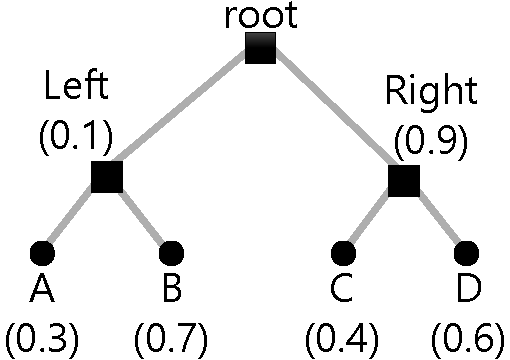
\includegraphics[width=\textwidth]{pifo_hpfq_example.pdf}
\caption{Algorithm}
\label{fig:hpfq_algo}
\end{subfigure}
\vrule
\begin{subfigure}[b]{.3\textwidth}
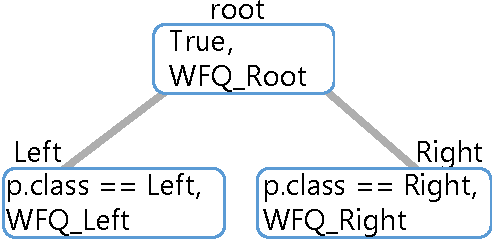
\includegraphics[width=\textwidth]{pifo_hpfq_program.pdf}
\caption{Scheduling tree}
\label{fig:hpfq_tree}
\end{subfigure}
\vrule
\begin{subfigure}[b]{.5\textwidth}
\begin{lstlisting}[style=customc]
f = flow(p) # see caption below
if f in last_finish:
  p.start = max(virtual_time, last_finish[f])
else:
  p.start = virtual_time
last_finish[f] = p.start + p.length / f.weight
p.rank = p.start
\end{lstlisting}
\caption{Scheduling transaction for WFQ\_Root, WFQ\_Left, and
  WFQ\_Right.}
\label{fig:hpfq_trans}
\end{subfigure}
\caption{Programming HPFQ using PIFOs. ``Left'' and ``Right'' are
  classes. A, B, C, and D are flows.  Within each tree node in the scheduling tree, the first
  line is the packet predicate and the second is the scheduling
  transaction. All three nodes execute the same code for the scheduling
  transaction except for their flow() function, which returns a packet's flow/class. For
  WFQ\_Root, it returns the packet's class: Left/Right. For WFQ\_Left
  and WFQ\_Right, it returns the packet's flow: A/B or C/D.}
\label{fig:hpfq}
\end{figure*}

We now describe the three main abstractions in our programming model. First, we
show how to use a {\em scheduling transaction} to program simple
work-conserving scheduling algorithms using a single PIFO~(\S\ref{ss:wfq}).
Second, we generalize to a {\em scheduling tree} to program hierarchical
work-conserving scheduling algorithms~(\S\ref{ss:hpfq}). Third, we augment
nodes of this tree with a {\em shaping transaction} to program
non-work-conserving scheduling algorithms~(\S\ref{ss:hshaping}).

\subsection{Scheduling transactions}
\label{ss:wfq}

A {\em scheduling transaction} is a block of code associated with a PIFO that
is executed once for each packet before the packet is enqueued. The scheduling
transaction computes the packet's rank, which determines its position in the
PIFO. Scheduling transactions can be used to program work-conserving scheduling
algorithms. In particular, a single scheduling transaction and PIFO are
sufficient to specify any scheduling algorithm where the relative scheduling
order of packets already present in the buffer does not change with the arrival
of future packets.

WFQ, described earlier (\S\ref{ss:decon_wfq}), is one example. It achieves
weighted max-min allocation of link capacity across flows sharing a link. We
define a flow to be any set of packets sharing common values for specific
packet fields.  Approximations to WFQ\footnote{An approximation is required
because the original WFQ algorithm~\cite{wfq} has a complex virtual time
calculation.} include Deficit Round Robin (DRR)~\cite{drr}, Stochastic Fairness
Queueing (SFQ)~\cite{sfq}, and Start-Time Fair Queueing (STFQ)~\cite{stfq}. We
consider STFQ here, and show how to program it using the scheduling transaction
in Figure~\ref{fig:sched_trans}.

Before a packet is enqueued, STFQ computes a {\em virtual start time} for that
packet (\texttt{p.start} in Figure~\ref{fig:sched_trans}) as the maximum of the
{\em virtual finish time} of the previous packet in that packet's flow
(\texttt{last\_finish[f]} in Figure~\ref{fig:sched_trans}) and the current
value of the {\em virtual time} (\texttt{virtual\_time} in
Figure~\ref{fig:sched_trans}), a state variable that tracks the virtual start
time of the last dequeued packet across all flows.\footnote{\S\ref{ss:add_impl}
discusses how this state variable can be accessed on the enqueue side.} Packets
are scheduled in order of increasing virtual start times, which is the packet's
rank in the PIFO.
%TODO: First sentence above is too wordy.

\subsection{Scheduling trees}
\label{ss:hpfq}

Scheduling algorithms that require changing the relative order of buffered
packets when a new packet arrives cannot be programmed using a single
scheduling transaction and PIFO. An important class of such algorithms are {\em
hierarchical} schedulers that compose multiple scheduling policies at different
levels of the hierarchy. We introduce a {\em scheduling tree} for such
algorithms.

To illustrate a scheduling tree, consider Hierarchical Packet Fair Queueing
(HPFQ)~\cite{hpfq}, a recursive variant of fair queueing. HPFQ first divides
link capacity fairly between classes, then recursively between sub classes in
each class, all the way down to the leaf nodes.  Figure~\ref{fig:hpfq_algo}
provides an example; the number on each child indicates its weight relative to
its siblings in its parent's fair scheduler.  HPFQ cannot be realized using a
single scheduling transaction and PIFO because the relative scheduling order of
packets that are already buffered can change with future packet arrivals.
Section 2.2 of the HPFQ paper~\cite{hpfq} provides an example illustrating how
this can happen.

HPFQ {\em can}, however, be realized using a tree of PIFOs, with a scheduling
transaction attached to each PIFO in the tree. To see how, observe that HPFQ
executes WFQ at each level of the hierarchy, with each node using WFQ among its
children. As discussed in \S\ref{ss:wfq}, a single PIFO encodes the current
scheduling order for WFQ, \ie the scheduling order if there are no further
arrivals. Similarly, a tree of PIFOs (Figure~\ref{fig:pifo_encoding}), where
each PIFO's elements are either packets or references to other PIFOs, can be
used to encode the current scheduling order of HPFQ and other hierarchical
scheduling algorithms. To determine this scheduling order, we inspect the root
PIFO to determine the next child PIFO to schedule. Then, we recursively inspect
the child PIFO to determine the next grandchild PIFO to schedule, until
reaching a leaf PIFO that determines the next packet to schedule.

\begin{figure}
\centering
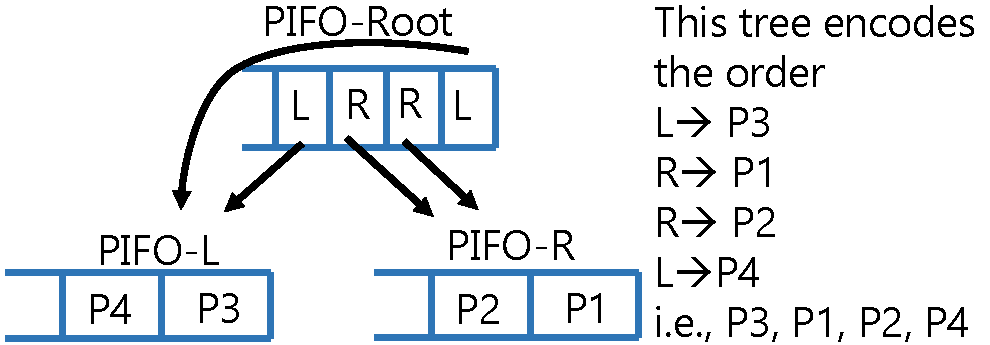
\includegraphics[width=0.45\textwidth]{pifo_pifo_tree_encoding.pdf}
\caption{PIFO trees encode current scheduling order for hierarchical schedulers.}
\label{fig:pifo_encoding}
\end{figure}

The current scheduling order of the PIFO tree can be modified as packets are
enqueued, by executing a scheduling transaction at each node in the PIFO tree.
This is our second programming abstraction: a {\em scheduling tree}.  Each node
in this tree is a tuple with two attributes. First, a packet predicate that
specifies which packets execute that node's scheduling transaction before
enqueueing an element into that node's PIFO; this element is either a packet or
a reference to a child PIFO of the node.  Second, a scheduling transaction that
specifies how the rank is computed for elements (packet or PIFO references)
that are enqueued into the node's PIFO. Figure~\ref{fig:hpfq_tree} shows an
example for HPFQ.

When a packet is enqueued into a scheduling tree, it executes one transaction
at each node whose packet predicate matches the arriving packet. These nodes
form a path from a leaf to the root of the tree and the transaction at each
node on this path updates the scheduling order at that node. One element is
enqueued into the PIFO at each node on the path from the leaf to the root. At
the leaf node, that element is the packet itself; at the other nodes, it is a
reference to the next PIFO on the path towards the leaf. Packets are dequeued
in the order encoded by the tree of PIFOs~(Figure~\ref{fig:pifo_encoding}).

\subsection{Shaping transactions}
\label{ss:hshaping}

%%% Figure for hshaping below %%%
\begin{figure*}
\begin{subfigure}[b]{0.2\textwidth}
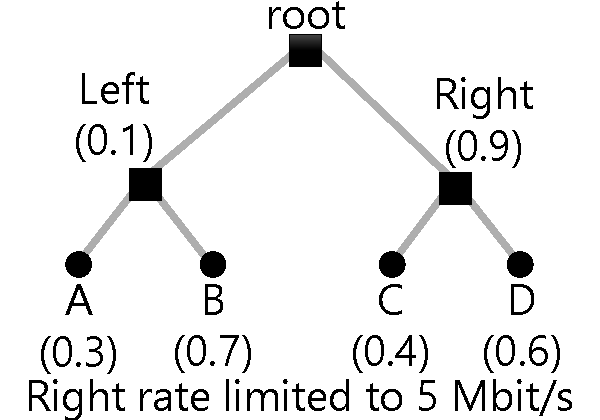
\includegraphics[width=\textwidth]{pifo_hshaping_example.pdf}
\caption{Algorithm}
\label{fig:hshaping_algo}
\end{subfigure}
\vrule
\begin{subfigure}[b]{0.3\textwidth}
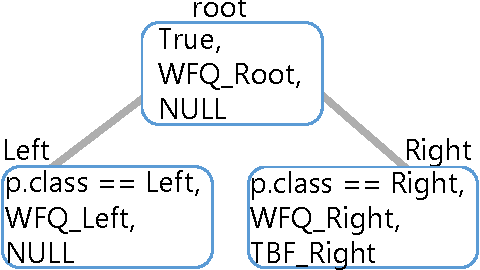
\includegraphics[width=\textwidth]{pifo_hshaping_program.pdf}
\caption{Scheduling tree}
\label{fig:hshaping_tree}
\end{subfigure}
\vrule
\begin{subfigure}[b]{0.5\textwidth}
\begin{lstlisting}[style=customc]
tokens = tokens + r * (now - last_time)
if (tokens > B):
  tokens = B
if (p.length <= tokens):
  p.send_time = now
else:
  p.send_time = now + (p.length - tokens) / r
tokens = tokens - p.length
last_time = now
p.rank = p.send_time
\end{lstlisting}
\caption{Shaping transaction for TBF\_Right.}
\label{fig:hshaping_shaping_trans}
\end{subfigure}
\caption{Programming Hierarchies with Shaping using PIFOs. The third line
within each tree node in the scheduling tree is the shaping transaction. The
scheduling transactions for WFQ\_Right, WFQ\_Left, and WFQ\_Root are identical
to Figure~\ref{fig:hpfq}.}
\label{fig:hshaping}
\end{figure*}

So far, we have only considered work-conserving scheduling algorithms. {\em
Shaping transactions} allow us to program non-work-conserving scheduling
algorithms. Non-work-conserving algorithms differ from work-conserving
algorithms in that they decide the {\em time} at which packets are scheduled as
opposed to the scheduling {\em order}. As an example, consider the algorithm
shown in Figure~\ref{fig:hshaping_algo}, which extends the previous HPFQ
example with the requirement that the Right class be limited to 5~Mbit/s. We
refer to this example as {\em Hierarchies with Shaping}.

To motivate our abstraction for non-work-conserving algorithms, recall that a
PIFO tree encodes the current scheduling order, by walking down the tree from
the root PIFO to a leaf PIFO to schedule packets.  With this encoding, a PIFO
reference can be scheduled only if it resides in a PIFO and there is a chain of
PIFO references from the root PIFO to that PIFO reference. To program
non-work-conserving scheduling algorithms, we provide the ability to {\em
defer} when a PIFO reference is enqueued into the PIFO tree, and hence is
available for scheduling.

To defer enqueues into the PIFO tree, we augment nodes of the scheduling tree
with an optional third attribute: a {\em shaping transaction} that is executed
on all packets matched by the node's packet predicate. The shaping transaction
on a node determines when a reference to the node's PIFO is available for
scheduling in the node's {\em parent's} PIFO. The shaping transaction is
implemented using a separate {\em shaping PIFO} at the child---distinct from
the scheduling PIFO at all nodes---that holds references to the child's
scheduling PIFO until they are released to the parent's scheduling PIFO.  The
shaping transaction uses the wall-clock departure time as the rank for the
shaping PIFO, unlike the scheduling transaction that uses the relative
scheduling order as the rank.

Once a reference to the child's scheduling PIFO has been released to the
parent's scheduling PIFO from the child's shaping PIFO, it is scheduled by
executing the parent's scheduling transaction and enqueueing it in the parent's
scheduling PIFO. If a node has no shaping transaction, references to that
node's scheduling PIFO are immediately enqueued into its parent's scheduling
PIFO with no deferral.  The dequeue logic during shaping still follows
Figure~\ref{fig:pifo_encoding}: dequeue recursively from the root until we
schedule a packet.

%Anirudh->Mohammad; I think we are complicating things by repeatedly saying packet (or PIFO
%reference) It's correct to just say PIFO reference and forget about packets altogether.
% It makes for simpler semantics as well.
% It just mandates that even rate limiting a single flow will now need three PIFOs, as given below, but that's fine
% Child: shaping PIFO releases references to Child's scheduling PIFO to parent
% Child: scheduling PIFO holds packets.
% Parent's scheduling PIFO executes First-in First-Out across references of Child's scheduling PIFO.
% This is a complicated way of implementing shaping at one level, but it simplifies semantics
% because only PIFO references can now be enqueue into the parent's scheduling PIFO, not packets.

Figure~\ref{fig:hshaping_shaping_trans} shows an example of a shaping
transaction that defers enqueues based on a Token Bucket Filter (TBF)
with a rate-limit of $r$ and a burst allowance $B$. Here, the packet's
wall clock departure time ({\tt p.send\_time}), is used as its rank in
the shaping PIFO. Figure~\ref{fig:hshaping_tree} shows how to use this
shaping transaction to program Hierarchies with Shaping: the TBF
shaping transaction (TBF\_Right) determines when PIFO references for
Right's scheduling PIFO are released to Root's scheduling PIFO.

\begin{figure}[!t]
  \centering
  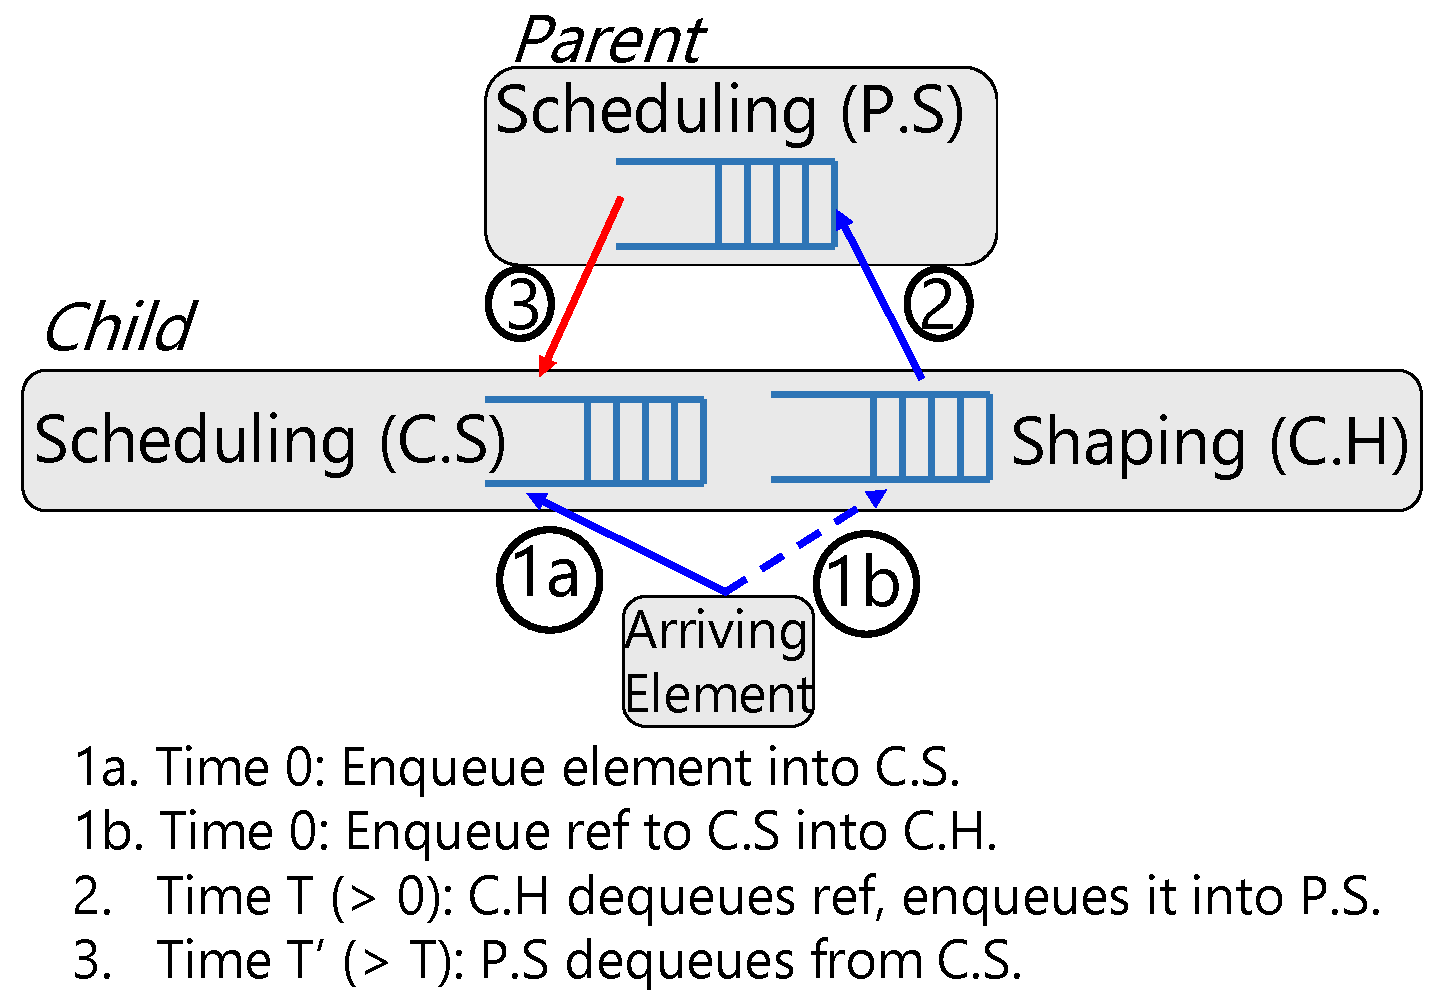
\includegraphics[width=0.6\columnwidth]{pifo_shaping_semantics.pdf}
  \caption{\textit{Child's} shaping transaction (1b) {\em defers} enqueue
  into \textit{Parent's} scheduling PIFO (2) until time T.  Blue arrows
  show enqueue paths. Red arrows show dequeue paths.  }
  \label{fig:shaping_trans}
\end{figure}

\Para{Timing of operations during shaping.}
We now describe the timing of operations during shaping in greater detail.
When a packet is enqueued in a tree of PIFOs, it executes a scheduling
transaction at the leaf node whose predicate matches this packet.  It then
continues upward towards the root executing scheduling transactions along the
path, until it reaches the first node that also has a shaping transaction
attached to it. Figure~\ref{fig:shaping_trans} shows the operations that occur
at this node, {\em Child}, and its parent, {\em Parent}, to implement shaping.

Two transactions are executed at {\em Child}: the original scheduling
transaction to push an element into {\em Child}'s scheduling PIFO (step 1a in
Figure~\ref{fig:shaping_trans}) and a shaping transaction to push an element
$R$ (step 1b), which is a reference to {\em Child}'s scheduling PIFO, into {\em
Child}'s shaping PIFO. After $R$ is pushed into {\em Child}'s shaping PIFO,
further transactions for this packet are suspended until $R$'s rank, the
wall-clock time $T$, is reached.

At $T$, $R$ will be dequeued from {\em Child}'s shaping PIFO and enqueued into
{\em Parent}'s scheduling PIFO (step 2), making it available for scheduling at
{\em Parent}. The rest of the packet's path to the root is now resumed starting
at {\em Parent}. This suspend-resume process can occur multiple times if there
are multiple nodes with shaping transactions along a packet's path from its
leaf to the root.

\section{The expressiveness of PIFOs}
\label{s:expressive}

In addition to the three examples from \S\ref{s:pifo}, we now provide several
more examples of scheduling algorithms that can be expressed using our
programming model (\S\ref{ss:lstf} through \S\ref{ss:other}) and also describe
the limitations of our programming model (\S\ref{pifo_ss:limitations}).

\subsection{Least Slack-Time First}
\label{ss:lstf}

Least Slack-Time First (LSTF)~\cite{lstf,ups} schedules packets at each router
in increasing order of packet slacks, \ie the time remaining until each
packet's deadline.  Packet slacks are initialized at an end host or edge router
and are decremented by the wait time at each router's queue. We can program
LSTF using a simple scheduling transaction:
\begin{lstlisting}[style=customc]
  p.rank  = p.slack + p.arrival_time
\end{lstlisting}

The addition of the packet's arrival time to the slack already carried in the
packet ensures that packets are dequeued in order of their slack at the time of
dequeue, not enqueue. Then, after packets are dequeued, we subtract the time at
which the packet is dequeued from the packet's slack, which has the effect of
decrementing the slack by the wait time at the router's queue. This subtraction
can be achieved by programming the egress pipeline to decrement one header
field by another using the techniques from Chapter~\ref{chap:domino}.

\subsection{Stop-and-Go Queueing}
\label{ss:stopngo}

\begin{figure}[h]
  \begin{lstlisting}[style=customc]
  if (now >= frame_end_time):
    frame_begin_time = frame_end_time
    frame_end_time   = frame_begin_time + T
  p.rank = frame_end_time
  \end{lstlisting}
\caption{Shaping transaction for Stop-and-Go Queueing.}
\label{fig:stopngo}
\end{figure}

Stop-and-Go Queueing~\cite{stopngo} is a non-work-conserving algorithm that
provides bounded delays to packets using a framing strategy. Time is divided
into non-overlapping frames of equal length \texttt{T}, where every packet
arriving within a frame is transmitted at the end of the frame, smoothing out
any burstiness in traffic patterns induced by previous hops.

The shaping transaction in Figure~\ref{fig:stopngo} can be used to program
Stop-and-Go Queueing. {\tt frame\_begin\_time} and {\tt frame\_end\_time} are
two state variables that track the beginning and end of the current frame in
wall-clock time.  When a packet is enqueued, its departure time is set to the
end of the current frame.  Multiple packets with the same departure time are
sent out in first-in first-out order, as guaranteed by a PIFO's semantics for
breaking ties with equal ranks (\S\ref{s:pifo}).

\subsection{Minimum rate guarantees}
\label{ss:min_rate}

A common scheduling policy on many routers today is providing a minimum rate
guarantee to a flow, provided the sum of such guarantees does not exceed the
link capacity. A minimum rate guarantee can be programmed using PIFOs with a
two-level PIFO tree, where the root of the tree implements strict priority
scheduling across flows. Flows below their minimum rate are scheduled
preferentially to flows above their minimum rate. Then, at the next level of
the tree, the PIFOs implement the FIFO discipline for each flow.

When a packet is enqueued, we execute a scheduling transaction corresponding to
the FIFO discipline at its leaf node, setting its rank to the wall-clock time
on arrival. At the root, a PIFO reference (the packet's flow identifier) is
pushed into the root PIFO using a rank that reflects whether the flow is above
or below its rate limit after the arrival of the current packet. To determine
this, we run the scheduling transaction in Figure~\ref{fig:min_rate} that uses
a token bucket (the state variable {\tt tb}) that can be filled up until {\tt
BURST\_SIZE} to decide if the arriving packet puts the flow above or below {\tt
min\_rate}.

\begin{figure}
  \begin{lstlisting}[style=customc]
  # Replenish tokens
  tb = tb + min_rate * (now - last_time)
  if (tb > BURST_SIZE):
    tb = BURST_SIZE

  # Check if we have enough tokens
  if (tb > p.size):
    p.over_min = 0 # under min. rate
    tb = tb - p.size
  else:
    p.over_min = 1 # over min. rate

  last_time = now
  p.rank = p.over_min
  \end{lstlisting}
\caption{Scheduling transaction for minimum rate guarantees.}
\label{fig:min_rate}
\end{figure}

Note that a single PIFO node with the scheduling transaction in
Figure~\ref{fig:min_rate} is not sufficient. It causes packet
reordering within a flow: an arriving packet can cause a flow to move
from a lower to a higher priority and, in the process, leave before
low priority packets from the same flow that arrived earlier. The
two-level tree solves this problem by attaching priorities to
transmission opportunities for a specific flow, not specific
packets. Now if an arriving packet causes a flow to move from low to
high priority, the next packet scheduled from this flow is the
earliest packet of that flow chosen in FIFO order, not the arriving
packet.

\subsection{Other examples}
\label{ss:other}

We now briefly describe several more scheduling algorithms that can be
programmed using PIFOs.

\begin{CompactEnumerate}
\item \textbf{Fine-grained priority scheduling.} Many algorithms
  schedule the packet with the lowest value of a field initialized by
  the end host. These algorithms can be programmed by setting the
  packet's rank to the appropriate field. Examples of such algorithms
  and the fields they use are strict priority scheduling (IP TOS
  field), Shortest Flow First (flow size), Shortest Remaining
  Processing Time (remaining flow size), Least Attained Service (bytes
  received for a flow), and Earliest Deadline First (time until a
  deadline).
\item \textbf{Service-Curve Earliest Deadline First
    (SC-EDF)~\cite{sced}} schedules packets in increasing order of a
  deadline computed from a flow's service curve, which specifies the
  service a flow should receive over any given time interval. We can
  program SC-EDF using a scheduling transaction that sets a packet's
  rank to the deadline computed by the SC-EDF algorithm.
\item \textbf{Rate-Controlled Service Disciplines (RCSD)~\cite{rcsd}}
  such as Jitter-EDD~\cite{jitteredd} and Hierarchical Round
  Robin~\cite{hrr} are a class of non-work-conserving schedulers
  that can be implemented using a combination of a rate
  regulator to shape traffic and a packet scheduler to schedule the
  shaped traffic. An RCSD algorithm can be programmed using PIFOs by
  programming the rate regulator using a shaping transaction and the
  packet scheduler using a scheduling transaction.
  
\item \textbf{Incremental deployment.}
  Operators may wish to use programmable scheduling only for a
  subset of their traffic. This can be programmed as a hierarchical
  scheduling algorithm, with one FIFO class dedicated to legacy
  traffic and another to experimental traffic. Within the experimental
  class, an operator could program any scheduling tree, \eg WFQ, LSTF, HPFQ.
\end{CompactEnumerate}

\subsection{Limitations}
\label{pifo_ss:limitations}

\Para{Changing the scheduling order of all packets of a flow.} 
Although a tree of PIFOs can enable algorithms where the relative scheduling order
of buffered packets changes in response to new packet arrivals (\S\ref{ss:hpfq}), it
does not permit arbitrary changes to the scheduling order of buffered
packets. In particular, it does not support changing the scheduling
order for {\em all} buffered packets of a flow when a new packet from
that flow arrives.

An example of an algorithm that needs this capability is
pFabric~\cite{pFabric}, which introduces ``starvation prevention'' to
schedule the packets of the flow with the shortest remaining size in
FIFO order, in order to prevent packet reordering. To see why this is beyond
the capabilities of PIFOs, consider the sequence of arrivals below,
where pi(j) represents a packet from flow i with remaining size j,
where the remaining size is the number of unacknowledged bytes in a flow.
\begin{CompactEnumerate}
\item Enqueue p0(7).
\item Enqueue p1(9), p1(8).
\item The scheduling order is: p0(7), p1(9), p1(8).
\item Enqueue p1(6).
\item The new order is: p1(9), p1(8), p1(6), p0(7).
\end{CompactEnumerate}

Specifying these semantics are beyond the capabilities of the PIFO
abstractions we have developed.\footnote{This is ironic because we
  started this project to implement pFabric in a programmable manner, and
  have ended up being able to do almost everything but that!} For
instance, adding a level of hierarchy with a PIFO tree does not
help. Suppose we programmed a PIFO tree implementing FIFO at the
leaves and picking among flows at the root based on the remaining flow
size. This would result in the scheduling order p1(9), p0(7), p1(8),
p1(6), after enqueuing p1(6). The problem is that there is no way to
change the scheduling order for {\em multiple} references to flow 1 in the
root PIFO by enqueuing only one reference to flow 1.
%% Mohammad: The above might still be too confusing; I know we don't
%% have much room, but a figure would really help with this. Let's run
%% this specifically by Jeff and Hari and see if it is comprehensible.
%% TODO: Yes, it's still a bit confusing. We could draw a figure.
%% Maybe we could remove CBQ to make room for this figure?

A single PIFO {\em can}, however, implement pFabric without starvation prevention,
which is identical to the Shortest Remaining Processing Time (SRPT) discipline
(\S\ref{ss:other}).  It can also implement the Shortest Flow First (SFF)
discipline (\S\ref{ss:other}), which performs almost as well as
pFabric~\cite{pFabric}.

\Para{Traffic shaping across multiple nodes in a scheduling tree.}  Our
programming model attaches a single shaping and scheduling transaction
to a tree node. This lets us enforce rate limits on a single node, but not
across multiple nodes.

As an example, PIFOs cannot express the following policy: WFQ on a set of flows
A, B, and C, with the additional constraint that the aggregate throughput of
A+B does not exceed 10 Mbit/s. One work around is to implement this as HPFQ
across two classes C1 and C2, with C1 containing A and B, and C2 containing C
alone. Then, we enforce the rate limit of 10 Mbit/s on C1 as in
Figure~\ref{fig:hshaping}. However, this is not equivalent to our desired
policy. More generally, our programming model for programmable scheduling
establishes a one-to-one relationship between the scheduling and shaping
transactions, which excludes some scheduling algorithms.

\Para{Output rate limiting.} The PIFO abstraction enforces rate limits using a
shaping transaction, which determines a packet or PIFO reference's scheduling
time {\em before} it is enqueued into a PIFO.  The shaping transaction permits
rate limiting on the {\em input} side, \ie before elements are enqueued. An
alternate form of rate limiting is on the {\em output}, \ie by limiting the
rate at which elements are scheduled.

To illustrate the difference, consider a scheduling algorithm with two
priority queues, \texttt{LO} and \texttt{HI}, where \texttt{LO} is to
be rate limited to 10 Mbit/s. To program this using input side rate
limiting, we would use a shaping transaction to impose a 10 Mbit/s
rate limit on \texttt{LO} and a scheduling transaction to implement
strict priority scheduling between \texttt{LO} and \texttt{HI}. Now,
assume packets from \texttt{HI} starve \texttt{LO} for a long
period of time. During this time, packets from \texttt{LO}, after
leaving the shaping PIFO, accumulate in the PIFO shared with
\texttt{HI}. Now, if there are suddenly no more \texttt{HI} packets,
all packets from \texttt{LO} are transmitted at line rate, and are no
longer rate limited to 10 Mbit/s for a transient period of time,
\ie until all instances of \texttt{LO} are drained out of the PIFO
shared with \texttt{HI}. Input rate limiting still provides long-term
rate guarantees, while output rate limiting provides short-term
guarantees as well.

\section{Design}
\label{s:design}

\begin{figure*}
  \centering
  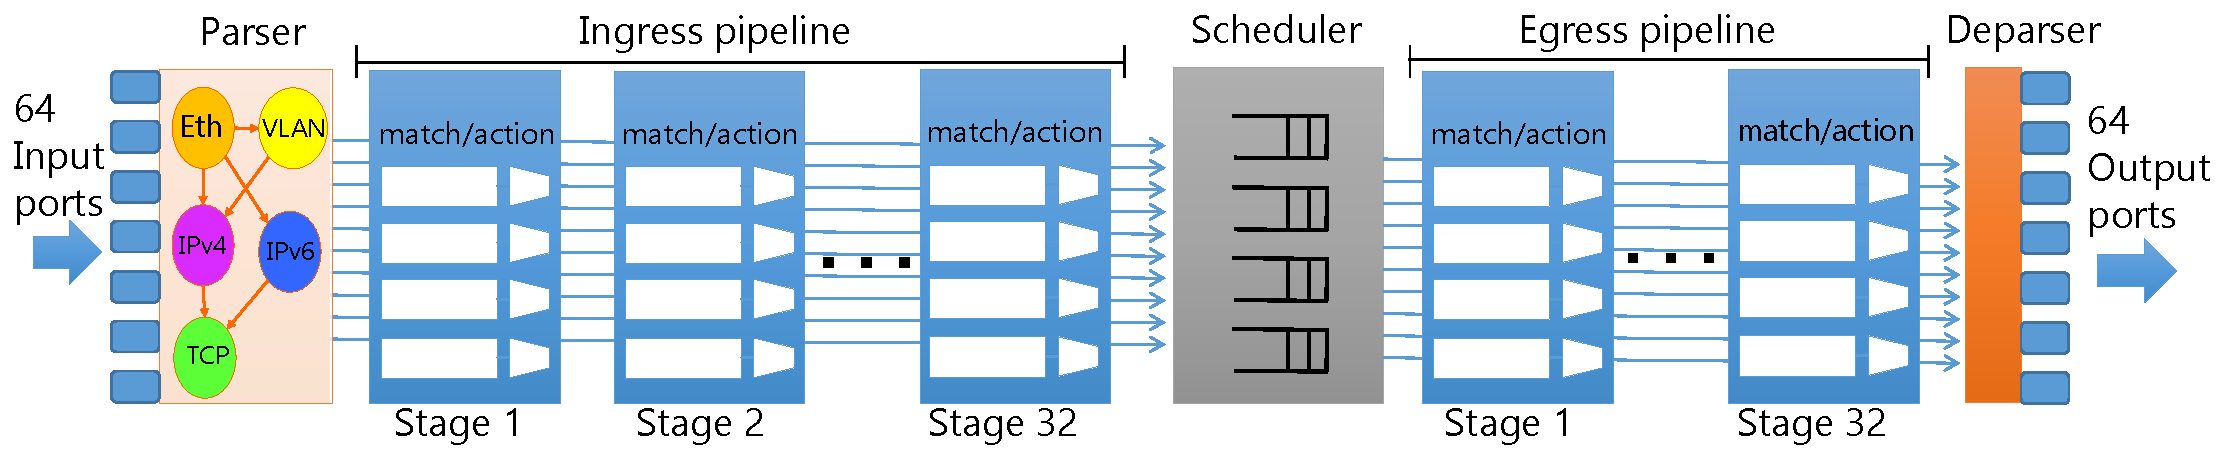
\includegraphics[width=\textwidth]{pifo_router_pipeline.pdf}
  \caption{A shared memory router.  Combinational logic and memory are
  shared across ports, both in the pipelines and in the scheduler.}
%The router runs at a clock frequency of 1 GHz.}
  \label{pifo_fig:router}
\end{figure*}

We now present a hardware design for a programmable scheduler based on PIFOs.
We target shared-memory routers such as Broadcom's Trident II~\cite{trident2}
(Figure~\ref{pifo_fig:router}). In these routers, a parser feeds packets from
all ports into a shared ingress pipeline, after which they enter a shared
scheduler and a similarly shared egress pipeline. To reduce chip area,
combinational logic and memory for packet processing are shared across ports,
both in the pipelines and in the scheduler. As discussed earlier
(\S\ref{s:absmachine}), the number of pipelines depends on the aggregate
capacity of the router. For our PIFO design, we focus on a 64-port 10G
single-pipeline router, where one pipeline handles the aggregate processing
requirements of all ports at minimum packet size, \ie 64 10 Gbit/s ports each
transmitting 64 byte packets. This translates into \textasciitilde 1 billion
packets per second, after accounting for minimum inter-packet gaps, or a 1 GHz
clock frequency.

We first describe how scheduling and shaping transactions can be implemented
(\S\ref{ss:transactions}). Then, we show how a tree of PIFOs can be realized
using a full mesh of {\em PIFO blocks} by appropriately interconnecting these blocks
(\S\ref{ss:mesh}). We also describe how a compiler (\S\ref{pifo_ss:compiler}) could
automatically configure this mesh from a scheduling tree.

\subsection{Scheduling and shaping transactions}
\label{ss:transactions}
To program and implement scheduling and shaping transactions, we use Domino
(Chapter~\ref{chap:domino}). Domino allows us to express these transactions in
Domino's domain-specific language, using a compiler to compile the transactions
down to a pipeline of \absmachine atoms.  One of the examples used to evaluate
Domino in \S\ref{s:eval} is the STFQ transaction from
Figure~\ref{fig:sched_trans}.  Specifically, Table~\ref{tab:algos} shows that
the STFQ transaction can be run at 1 GHz on a router pipeline with the Pairs
atom.

%TODO: We need to evaluate this more thoroughly.
Similarly, we could use the Domino compiler to compile other scheduling and
shaping transactions to an atom pipeline.  For example, the transactions for
Token Bucket Filtering (Figure ~\ref{fig:hshaping_shaping_trans}), minimum rate
guarantees (\S\ref{ss:min_rate}), Stop-and-Go queueing (\S\ref{ss:stopngo}),
and LSTF (\S\ref{ss:lstf}), can all be expressed as Domino programs. They can
then be compiled to a router pipeline with a sufficiently expressive
atom. An important restriction in Domino is the absence of loops, which
precludes rank computations containing a loop with an unbounded iteration
count. We have not, however, encountered a scheduling or shaping transaction
requiring this capability.
% Loops with bounded iteration count can be unrolled.

\begin{figure}[!t]
  \centering
  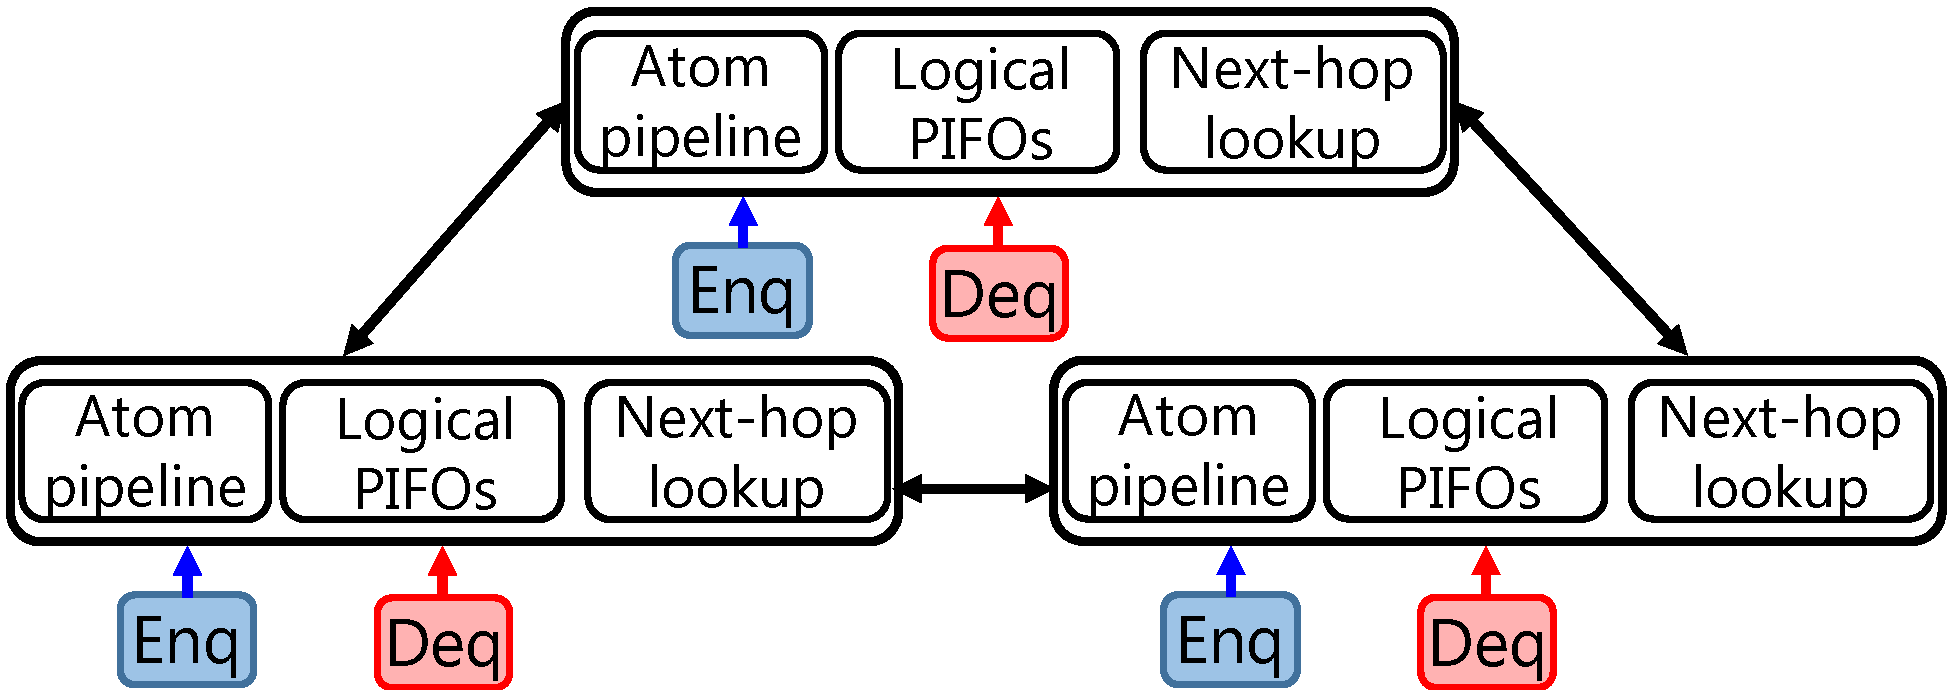
\includegraphics[width=0.6\columnwidth]{pifo_pifo_mesh.pdf}
  \caption{Three PIFO blocks in a PIFO mesh}
  \label{fig:mesh}
\end{figure}

\begin{figure}[!t]
  \centering
  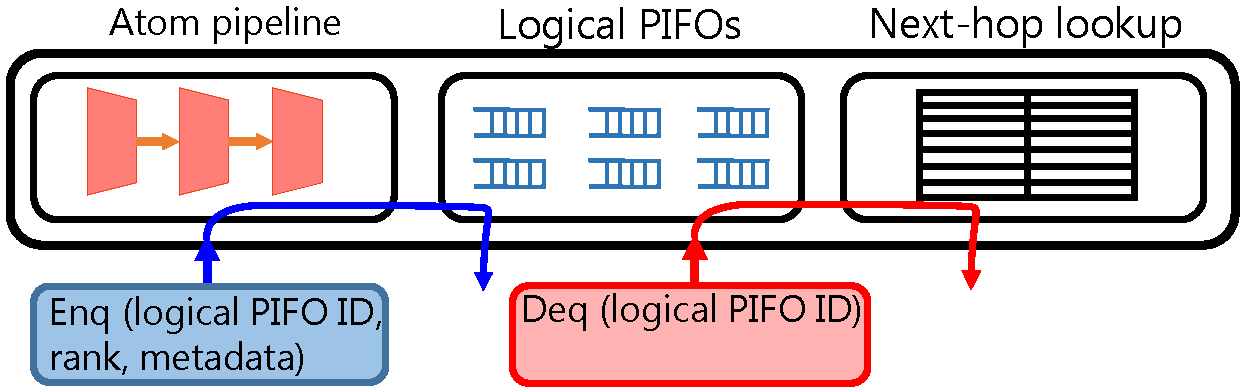
\includegraphics[width=0.6\columnwidth]{pifo_pifo_block.pdf}
  \caption{A single PIFO block. Enqueue operations execute transactions in the atom pipeline
  before enqueuing elements into a logical PIFO. Dequeue operations dequeue elements from logical PIFOs
  before looking up their next hop.} 
  \label{fig:block}
\end{figure}

\begin{figure*}[!t]
  \begin{subfigure}[b]{0.5\textwidth}
  \begin{center}
  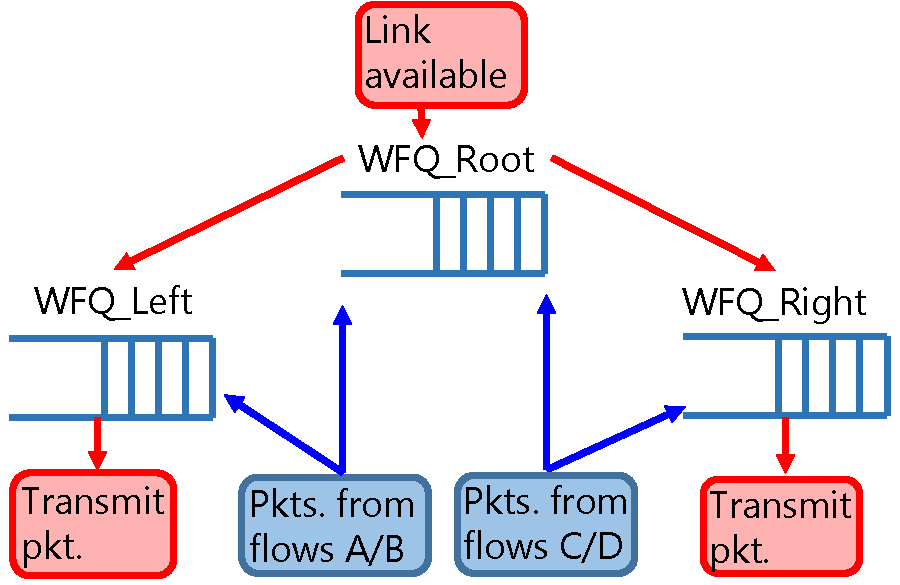
\includegraphics[width=\textwidth]{pifo_hpfq_logical.pdf}
  \caption{Logical PIFO tree for HPFQ}
  \label{fig:hpfq_path}
  \end{center}
  \end{subfigure}
  \begin{subfigure}[b]{0.5\textwidth}
  \begin{center}
  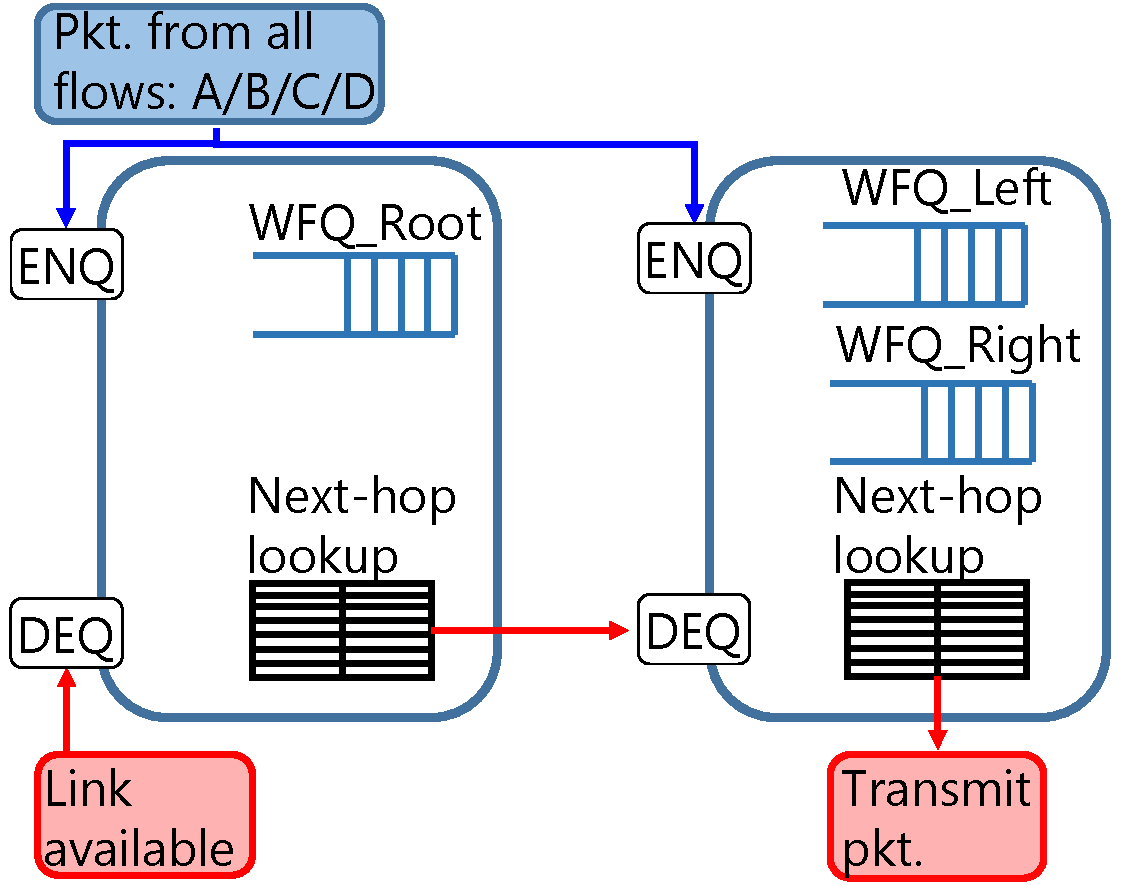
\includegraphics[width=0.8\textwidth]{pifo_hpfq_physical.pdf}
  \caption{Physical PIFO mesh for HPFQ}
  \label{fig:hpfq_mesh}
  \end{center}
  \end{subfigure}
  \caption{Compiling HPFQ (Figure~\ref{fig:hpfq}) to a PIFO mesh. On the left,
  the logical PIFO tree captures relationships between PIFOs: which PIFOs dequeue
  or enqueue into which PIFOs. Red arrows indicate dequeues, blue indicates
  enqueues.  On the right, we show the physical PIFO mesh for the logical PIFO
  tree on the left, following the same notation.}
  \label{fig:hpfq_compiling}
\end{figure*}

% Hopefully, this bit below they should have understood from earlier.
% All packets result in two enqueues: to the root
%  PIFO and one of the two leaf PIFOs. This is shown using two arrows starting
%  from one point (\eg the arrows originating from A/B).

\begin{figure*}[!t]
  \begin{subfigure}[b]{0.5\textwidth}
  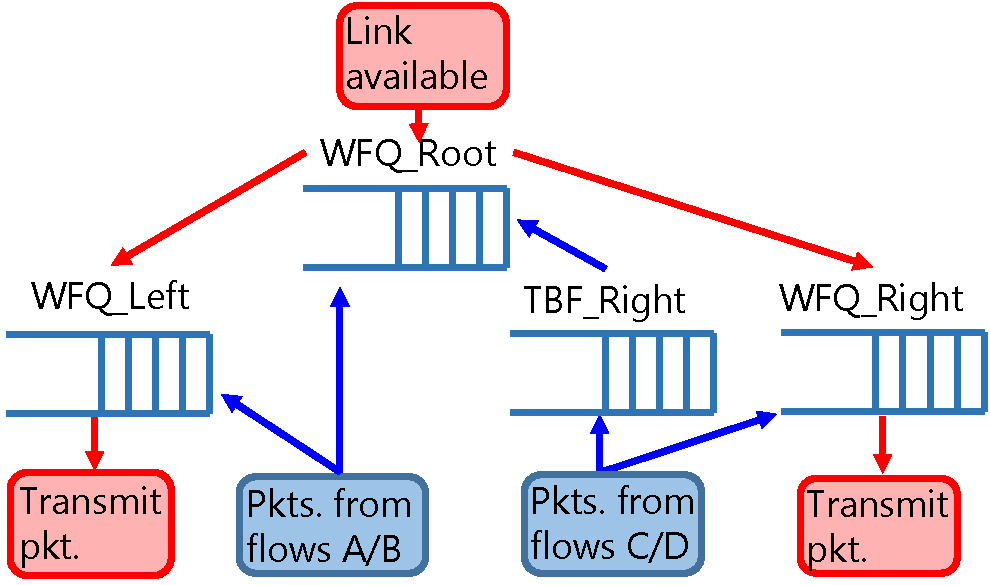
\includegraphics[width=\textwidth]{pifo_hshaping_logical.pdf}
  \caption{Logical PIFO tree for Hierarchies with Shaping}
  \label{fig:hshaping_path}
  \end{subfigure}
  \begin{subfigure}[b]{0.5\textwidth}
  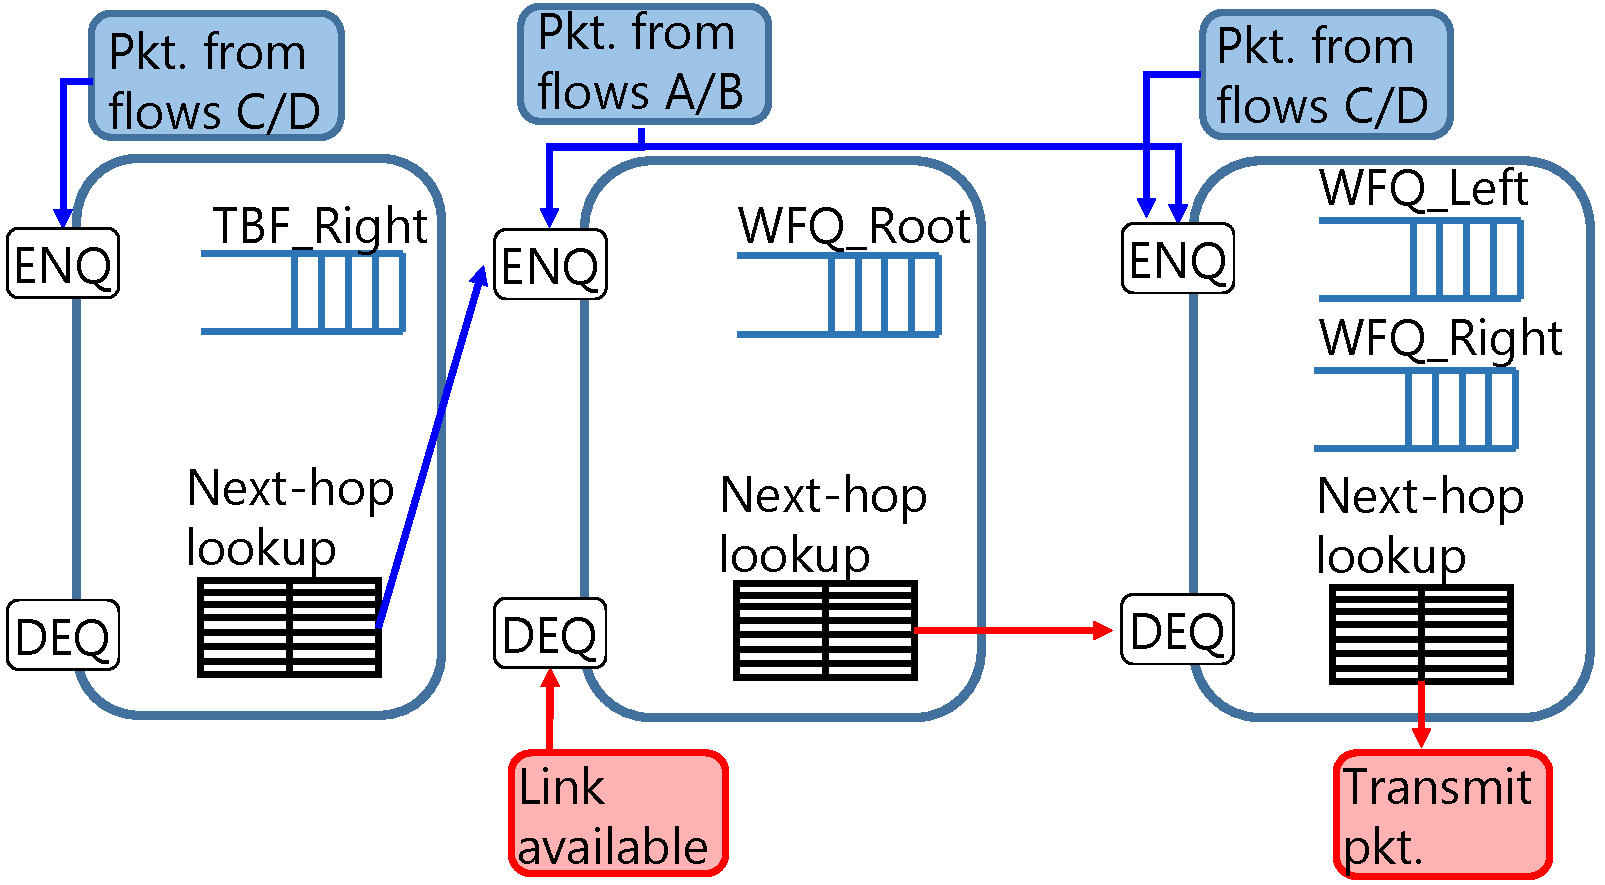
\includegraphics[width=\textwidth]{pifo_hshaping_physical.pdf}
  \caption{Physical PIFO mesh for Hierarchies with Shaping}
  \label{fig:hshaping_mesh}
  \end{subfigure}
  \caption{Compiling Hierarchies with Shaping (Figure~\ref{fig:hpfq}) to a PIFO mesh. Same comments as Figure~\ref{fig:hpfq_compiling} apply.}
\end{figure*}


\subsection{The PIFO mesh}
\label{ss:mesh}

%TODO: Define logical PIFO before.
We lay out PIFOs physically as a full mesh (Figure~\ref{fig:mesh}) of
{\em PIFO blocks} (Figure~\ref{fig:block}). Each PIFO block supports
multiple logical PIFOs. These logical PIFOs correspond to PIFOs for
different output ports or different classes in a
hierarchical scheduling algorithm, which share the combinational logic
required for a PIFO. We expect a small number of PIFO blocks in a
typical router (\eg fewer than five) because each PIFO block
corresponds to a different level of a hierarchical scheduling tree and
most practical hierarchical scheduling algorithms we know of do
  not require more than a few levels of hierarchy. As a result, a
full mesh between these blocks is feasible (\S\ref{ss:interconnect}
has more details).

% Maybe subsection for a PIFO block?
PIFO blocks run at 1 GHz and contain an atom
pipeline to execute scheduling and shaping transactions before enqueuing into a
logical PIFO. In every clock cycle, each PIFO block supports one enqueue and
dequeue operation on a logical PIFO residing within that block
(shaping transactions require more than one operation per clock cycle and
are discussed in \S\ref{ss:shape_challenge}). We address a logical PIFO within
a block with a logical PIFO ID.

The interface to a PIFO block is:
\begin{CompactEnumerate}
\item Enqueue an element (packet or reference to another PIFO) given a
  logical PIFO ID, the element's rank, and some metadata that will be
  carried with the element such as the packet length required for
  STFQ's rank computation. The enqueue returns nothing.
\item Dequeue from a specific logical PIFO ID within the block. The dequeue
   returns either a packet or a reference to another PIFO.
\end{CompactEnumerate}

After a dequeue, besides transmitting a packet, a PIFO block may
communicate with another PIFO block for two reasons:
 \begin{CompactEnumerate}
 \item To dequeue a logical PIFO in another block, \eg when dequeuing a
   sequence of PIFOs from the root to a leaf of a scheduling tree to transmit
   packets.
 
 \item To enqueue into a logical PIFO in another block, \eg when
   enqueuing a packet that has just been dequeued from a shaping
   PIFO.
 \end{CompactEnumerate}

We configure these post-dequeue operations using a small lookup table, which
looks up the ``next hop'' following a dequeue. This lookup table specifies an
operation (enqueue, dequeue, transmit), the PIFO block for the next operation,
and any arguments the operation needs.

\subsection{Compiling from a scheduling tree to a PIFO mesh}
\label{pifo_ss:compiler}

\an{A programmer should not have to manually configure a PIFO mesh. Instead, a
compiler translates from a scheduling tree to a PIFO mesh configuration implementing that tree.  While we haven't prototyped
this compiler, we illustrate how it would work using HPFQ (Figure~\ref{fig:hpfq})
and Hierarchies with Shaping (Figure~\ref{fig:hshaping}).}

The compiler first converts the scheduling tree to a logical PIFO tree that
specifies the enqueue and dequeue operations on each PIFO.
Figures~\ref{fig:hpfq_path} and \ref{fig:hshaping_path} show the logical PIFO tree for
the scheduling trees in Figures~\ref{fig:hpfq} and \ref{fig:hshaping} respectively.  It then overlays
this tree over a PIFO mesh by assigning every level of the tree to a PIFO block
and configuring the lookup tables to connect PIFO blocks as required by the
tree.  Figure~\ref{fig:hpfq_mesh} shows the PIFO mesh for
Figure~\ref{fig:hpfq}, while Figure~\ref{fig:hshaping_mesh} shows the PIFO mesh
for Figure~\ref{fig:hshaping}.

If a particular level of the tree has more than one enqueue or dequeue from
another level, which \an{arises in the presence of shaping transactions
(\S\ref{ss:shape_challenge})}, we allocate new PIFO blocks to respect the
constraint that any PIFO block provides only one enqueue and dequeue operation per
clock cycle, \eg Figure~\ref{fig:hshaping_mesh} has an additional PIFO block
containing TBF\_Right alone. Finally, we use the Domino compiler to compile
scheduling and shaping transactions.
%%
%%\footnote{More precisely, the shaping PIFO that the TBF\_Right
%%transaction enqueues into. We use a transaction's name to refer both to the
%%transaction and the PIFO it enqueues into.} 
%TODO: Could make above paragraph a bit more lucid.

\subsection{Challenges with shaping transactions}
\label{ss:shape_challenge}

Each PIFO block supports one enqueue and dequeue operation per clock cycle.
This suffices for any algorithm that only uses scheduling transactions
(work-conserving algorithms) because, for such algorithms, each packet needs at
most one enqueue and one dequeue at each level of its scheduling tree, and we
map the PIFOs at each level to a different PIFO block.

However, shaping transactions pose challenges. Consider Hierarchies with
Shaping (Figure~\ref{fig:hshaping_path}). When the shaping transaction enqueues
elements into TBF\_Right, these elements will be released into WFQ\_Root at a
future time $T$. The external enqueue into WFQ\_Root may also happen exactly at
$T$, if a packet arrives at $T$. This creates a conflict because there are two
enqueue operations in the same cycle.  Conflicts may also occur on dequeues.
For instance, if TBF\_Right shared its PIFO block with another logical PIFO,
dequeue operations to the two logical PIFOs could occur at the same time
because TBF\_Right can be dequeued at any arbitrary wall-clock time.

%%\MA{I think a transient variant of this problem exists with scheduling
%%  transactions as well if the PIFOs for different ports are not
%%  carefully placed. For example, if the WFQ\_Root PIFO for port 1 is in the
%%  same block as the WFQ\_Right PIFO for port 0, there could be a
%%  conflict. The difference (I think) is that this one is transient; it
%%  can't affect things by more than N clock cycles if there are N
%%  ports, so it wouldn't affect the line rate. We don't need to explain
%%  this, unless anyone else also wondered about this}

In a conflict, only one of the two operations can proceed. We resolve
this conflict in favor of scheduling PIFOs. Shaping PIFOs are used for
rate limiting to a rate lower than the line rate. Therefore, they
can afford to be delayed by a few clocks until there are no
conflicts. By contrast, delaying scheduling decisions of a scheduling PIFO
would mean that the router would idle and not satisfy its line-rate guarantee.


As a result, shaping PIFOs only get best-effort
service. There are workarounds to this. One is overclocking the pipeline at
(say) 1.25 GHz instead of 1 GHz, providing spare clock cycles for such
best-effort processing. Another is to provide multiple ports to a PIFO block to
support multiple operations every clock.  These techniques are commonly used in
routers for background tasks such as reclaiming buffer
space, and can be applied to the PIFO mesh as well.
% Amy wondered if there would be other kinds of conflicts, \ie shaping-shaping or scheduling-scheduling

\section{Hardware Implementation}
\label{s:hardware}
This section describes the hardware implementation of our programmable
scheduler. We discuss performance requirements
(\S\ref{ss:performance}), the implementation of a PIFO block
(\S\ref{ss:single_block}), and the full-mesh interconnect between them
(\S\ref{ss:interconnect}).  Finally, we estimate the additional chip area
incurred by our design (\S\ref{ss:feasibility}).

\subsection{Performance requirements}
\label{ss:performance}

\an{Our goal is a programmable scheduler competitive with common shared-memory
routers, such as the Broadcom Trident II~\cite{trident2}, used in many
datacenters today.  Based on the
Trident II, we target 1000 flows that can be flexibly allocated across logical
PIFOs and a 12 MByte packet buffer size~\cite{bcom_buffer} with a cell
size\footnote{Packets in a shared-memory router are allocated in small units
called cells.} of 200 bytes.  In the worst case, every packet is a single cell.
Hence, up to 60K packets/elements per PIFO block can be spread out over
multiple logical PIFOs.}

 Based on these requirements, our baseline design targets a PIFO block that
supports 64K packets and 1024 flows that can be shared across 256 logical
PIFOs. Further, we target a 16-bit rank field and a 32-bit metadata field
(\eg {\tt p.length} in Figure~\ref{fig:sched_trans}) for our PIFO block.
We put 5 such blocks together into a 5-block PIFO mesh that can
support up to 5 levels of hierarchy in a scheduling algorithm, sufficient for
most practical hierarchical schedulers we know of.

\begin{figure}[!t]
  \centering
  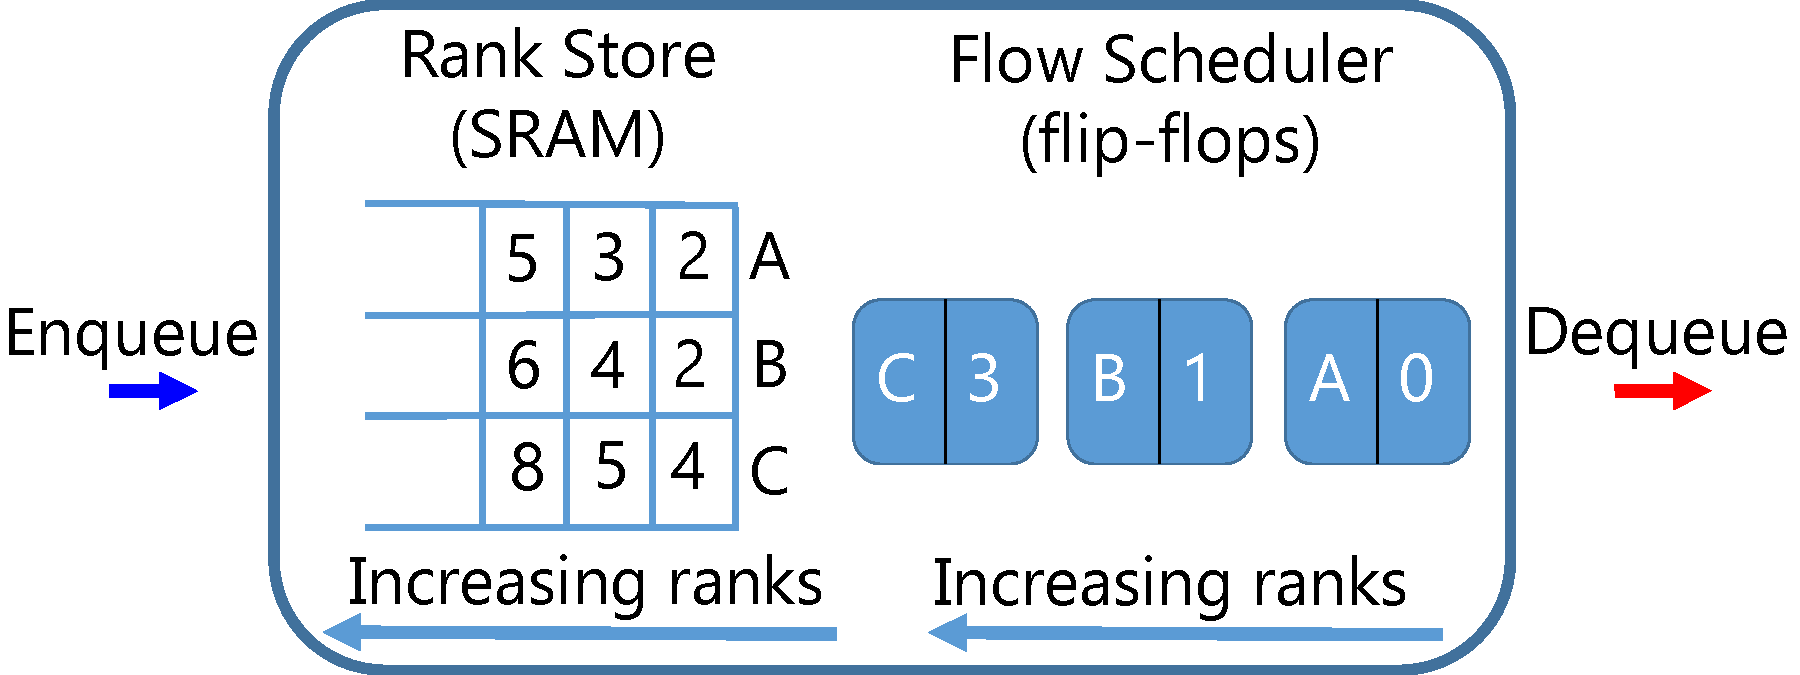
\includegraphics[width=0.6\columnwidth]{pifo_pifo_impl.pdf}
  \caption{Block diagram of PIFO block with a flow scheduler and a
   rank store. Logical PIFOs and metadata are not shown for simplicity.}
  \label{fig:pifo_impl}
\end{figure}

\subsection{A single PIFO block}
\label{ss:single_block}

A PIFO block supports two operations: an enqueue that inserts an element into a
logical PIFO and a dequeue to remove the head of a logical PIFO.  We first
consider two strawman designs for a PIFO: a flat sorted array and a
heap. We show how neither meets our requirements. We then describe an
implementation of a PIFO block with a single logical PIFO and then show how
it easily extends to multiple logical PIFOs in the same block.

One hardware implementation of a single PIFO is a flat sorted array. In this
implementation, an incoming element would be compared against all array elements
in parallel to determine a location for the new element, and then inserted
there by shifting the array.  However, each comparison needs one comparator
circuit, and supporting 64K parallel comparators is infeasible.

Another hardware implementation for a PIFO, which is essentially a priority
queue, is a heap in hardware. For instance, P-heap is a pipelined binary
heap scaling to 4-billion entries~\cite{bhagwan, pheap}. A capacity of 4 billion
 is more than sufficient for our needs.  However, each P-heap supports
traffic belonging to a {\em single} 10 Gbit/s input port in an input-queued
router; there is a separate P-heap instance for each port~\cite{bhagwan}.
Having a separate P-heap per port incurs prohibitive area overhead on a
shared-memory router, where the packet buffer and scheduling logic are shared
across all ports to reduce area overhead.  Conversely, we also found that it
was hard to overlay multiple logical PIFOs over a single P-heap, which would
allow the same physical P-heap to be shared across ports.

In contrast to the two strawman designs, our design for the PIFO exploits two
domain-specific characteristics. First, the packet buffers on shared-memory routers
used in datacenters today are much smaller (tens of megabytes) than those on
deep-buffered core routers (hundreds of megabytes) in the past.  This permits a
simpler, albeit less scalable, design relative to heaps. Second, there is
considerable structure in the ranks: nearly all practical scheduling algorithms
group packets into flows or classes, \eg based on traffic type, ports, or
addresses. They then schedule a flow's packets in FIFO order because packet
ranks increase across a flow's consecutive packets to prevent packet reordering within a flow. Thus, a PIFO needs to only
sort across the head packets of all flows, as opposed to all packets in the
buffer.\footnote{Last-In First-Out (LIFO) is a counterexample.  We can handle
LIFO by creating a new flow for every packet, so long as there are fewer than
1024 packets (flows) in the buffer at any time.}

This motivates a design with two parts (Figure~\ref{fig:pifo_impl}):
\begin{CompactEnumerate}
\item A {\em flow scheduler} that picks the next element to dequeue based on
the ranks of the {\em head} (earliest) elements of all flows. \an{The flow
scheduler is effectively a PIFO consisting of the head elements of all flows.}
\item A {\em rank store}, a FIFO bank that stores the ranks of elements beyond
the head for each flow in FIFO order.
\end{CompactEnumerate}

This decomposition reduces the number of elements requiring sorting from the
number of packets (64K) to the number of flows (1024). During an enqueue, an
element (both rank and metadata) is appended to the end of the appropriate FIFO
in the rank store. For a flow's first element, we bypass the rank store and
directly push it into the flow scheduler. To permit enqueues into this PIFO
block, we also supply a flow ID argument to the enqueue operation.

The FIFO bank needed for the rank store is a well-understood hardware design.
Such FIFO banks are used to buffer packet payloads in routers and much
engineering effort has gone into optimizing them.  As a result, we focus our
discussion here on the flow scheduler alone.

\Para{The flow scheduler.}
The flow scheduler sorts an array of flows using the ranks of the head elements
of all flows. It supports one enqueue {\em and} one dequeue to its enclosing
PIFO block every clock cycle, which translates into the following operations on
the flow scheduler every clock cycle.
\begin{CompactEnumerate}
  \item Enqueue operation: Inserting a flow into the flow scheduler 
  when the flow goes from empty to non-empty.
\item Dequeue operation: Removing a flow from the flow scheduuler that
  empties once it is scheduled, (or) removing and reinserting a flow into
  the flow scheduler with the rank of the
  next element if the flow is still backlogged.
\end{CompactEnumerate}

The operations above require the flow scheduler to internally support two
primitives every clock cycle.
\begin{CompactEnumerate}
\item {\em Push} up to two elements into the flow scheduler: one each for an
  enqueue's insert and a dequeue's reinsert.
\item {\em Pop} one element: for the remove from a dequeue.
\end{CompactEnumerate}
These primitives access all of the flow scheduler's elements in parallel. To
facilitate this, we implement the flow scheduler in flip flops, unlike the rank
store, which is in SRAM.

The flow scheduler is organized in hardware as a sorted array, where a push is
implemented by executing the three steps below
(Figure~\ref{fig:flow_scheduler}).
\begin{CompactEnumerate}
\item Compare the incoming rank against all ranks in the array in parallel, using a comparator.
  This produces a bit mask of comparison results indicating if the incoming rank
  is greater/lesser than an array element's rank.
\item Find the first 0-1 transition in this bit mask, using a priority encoder,
  to determine the index to push into.
\item Push the element into this index, by shifting the array.
\end{CompactEnumerate}
A pop is implemented by shifting the head element out of the sorted array.

So far, we have focused on a flow scheduler implementation handling a single
logical PIFO. To handle multiple logical PIFOs, we keep elements sorted by
rank, regardless of the logical PIFO they belong to; hence, the push logic
does not change.  To pop from a specific logical PIFO, we compare against all
elements to find elements with that logical PIFO ID. Among these, we find the
first using a priority encoder, and remove this element by shifting the array.
The rank store implementation does not change when introducing logical PIFOs;
however, we do require that a flow belong to exactly one logical PIFO.

%parallel and pipelined
To concurrently issue 2 pushes and 1 pop every clock cycle, we provision three
parallel digital circuits (Figure~\ref{fig:flow_scheduler}). Both the
push and pop require 2 clock cycles to complete and need to be pipelined
 to maintain the required throughput (Figure~\ref{fig:2stage}). For pushes, the first stage of the pipeline executes
the parallel comparison and priority encoder steps to determine an index; the
second stage pushes the element into the array using the index.  Similarly, for
pops, the first stage executes the equality check (for logical PIFO IDs) and
priority encoder steps to compute an index; the second stage pops the head
element out of the array using the index.

Our implementation meets timing at 1 GHz and supports up to one enqueue/dequeue
operation on a logical PIFO within a PIFO block every clock cycle. Because a
reinsert operation requires a pop, followed by an access to the rank store for
the next element, followed by a push, our implementation supports a dequeue
from the same logical PIFO only once every 4 cycles. This is because if a dequeue is initiated
in clock cycle 1, the pop for the dequeue completes in 2, the rank store is accessed in 3, and
the push is initiated in 4, making cycle 5 the earliest time to reissue a dequeue.
This restriction is inconsequential in practice.  A dequeue every 4 cycles from
a logical PIFO is sufficient to service the highest link speed today, 100
Gbit/s, which requires a dequeue at most once every 5 clock cycles for a
minimum packet size of 64 bytes. Dequeues to distinct logical PIFO IDs are
still permitted every cycle.

\begin{figure}[!t]
  \centering
  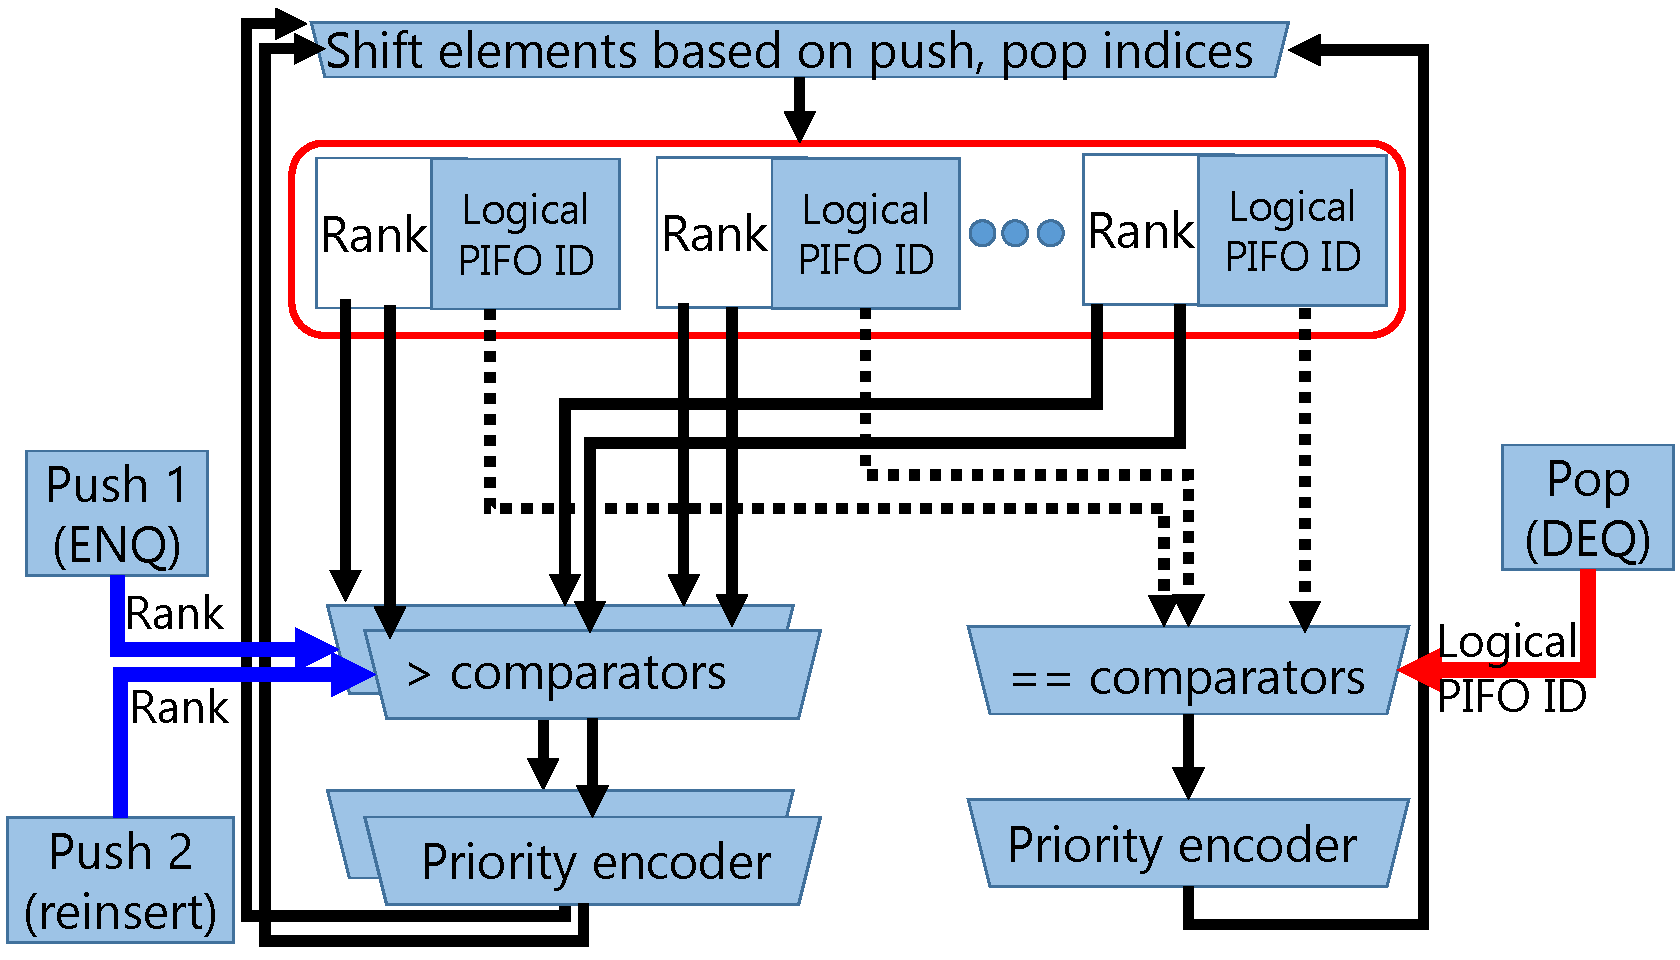
\includegraphics[width=0.6\columnwidth]{pifo_flow_scheduler_hardware.pdf}
  \caption{Hardware implementation of flow scheduler. Each element in the flow
  scheduler is connected to two > comparators (2 pushes) and one == comparator (1
  pop).}
  \label{fig:flow_scheduler}
\end{figure}

\begin{figure}[!t]
  \centering
  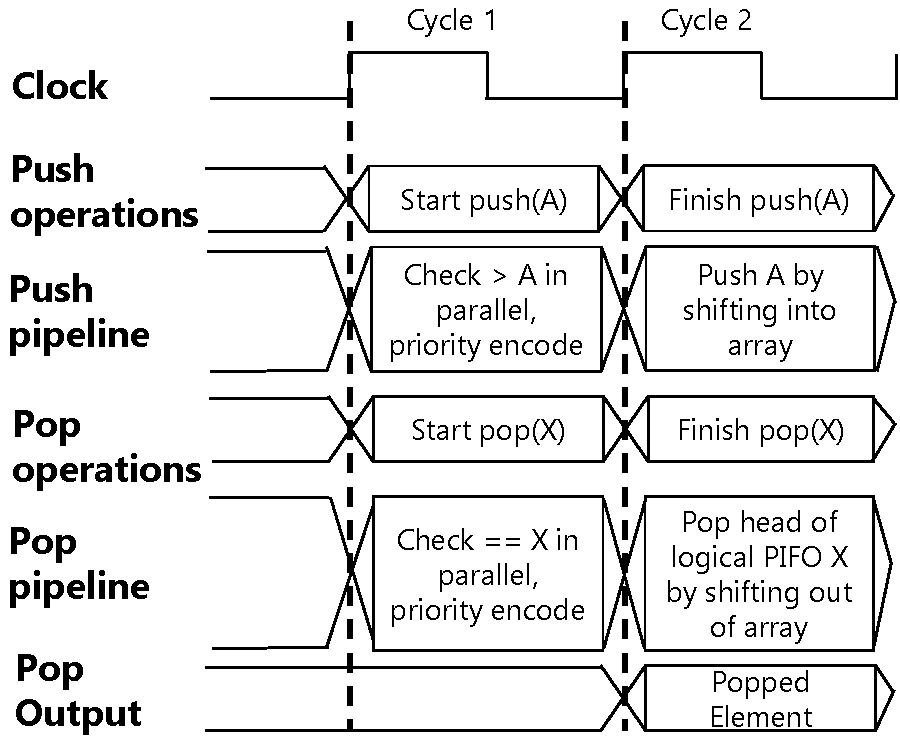
\includegraphics[width=0.6\columnwidth]{pifo_2stage_pipeline.pdf}
  \caption{2-stage pipeline for flow scheduler}
  \label{fig:2stage}
\end{figure}

\subsection{Interconnecting PIFO blocks}
\label{ss:interconnect}

An interconnect between PIFO blocks allows PIFO blocks to enqueue into and
dequeue from other blocks. Because the number of PIFO blocks is small, we
provide a full mesh between them. For a 5-block PIFO mesh as in our baseline
design, this requires 5*4 = 20 sets of wires between PIFO blocks. Each set
carries all the inputs required for specifying an enqueue and dequeue operation
on a PIFO block.

For our baseline design (\S\ref{ss:performance}), for an enqueue, we require a
logical PIFO ID (8 bits), the element's rank (16 bits), the element meta data
(32 bits), and the flow ID (10 bits). For a dequeue, we need a logical PIFO ID
(8 bits) and wires to store the dequeued element's metadata field (32 bits).
This adds up to 106 bits per set of wires, or 2120 bits for the mesh. This is a
small number of wires for an entire chip.  For example, RMT's match-action pipeline
uses 4000 1-bit wires between a {\em a pair of pipeline stages} to move its 4K
packet header vector between stages~\cite{rmt}. 

\subsection{Area overhead}
\label{ss:feasibility}

Because we target a shared-memory router, the scheduling logic is shared
across ports and a single PIFO mesh services an entire router. Therefore, to
estimate the area overhead of a programmable scheduler, we estimate the area
overhead of a single PIFO mesh. Our overhead does not have to be multiplied by
the number of ports and is the same for two shared-memory routers with equal
aggregate packet rates, \eg a 6-port 100G router and a 60-port 10G router.

%TODO: Why are next-hop tables small?
To determine the area of a PIFO mesh, we compute the area of a single PIFO
block and multiply it by the number of blocks because the area of the
interconnect itself is negligible.  For a single block's area, we separately
estimate areas for the rank store, atom pipelines, and flow scheduler, and
ignore the area of the small next-hop lookup tables.  We estimate the rank
store's area by using SRAM estimates~\cite{sram_estimate}, the atom pipeline's
area using the individual atom area numbers from Table~\ref{tab:templates}, and
the flow scheduler's area by implementing it in Verilog~\cite{system_verilog}
and synthesizing it to gate-level netlist in a 16-nm standard cell library
using the Cadence Encounter RTL Compiler~\cite{cadence_rc}. The RTL Compiler
also verifies that the flow scheduler meets timing at 1 GHz.

Overall, our baseline design consumes about 7.35 \si{\milli\metre\squared} of
chip area (Table~\ref{tab:area_overheads}). This is about 3.7\% of the chip
area of a typical router chip, using the minimum chip area estimate of 200
\si{\milli\metre\squared} provided by Gibb et al.~\cite{glen_parsing}. In
return for this 3.7\%, we get a significantly more flexible packet scheduler
than current routers, which provide {\em fixed} two or three-level hierarchical
scheduling. Our 3.7\% area overhead is similar to the overhead for other
programmable router functions, \eg 2\% for programmable
parsing~\cite{glen_parsing} and 15\% for programmable header
processing~\cite{rmt}.
 
\begin{table}[!h]
  \centering
  \begin{small}
  \begin{tabular}{|p{0.36\textwidth}|p{0.5\textwidth}|}
  \hline
  Component & Area in \si{\milli\metre\squared}\\
  \hline
  Router chip & 200--400~\cite{glen_parsing} \\
  \hline
  Flow Scheduler & 0.224 (from synthesis) \\
  \hline
  SRAM (1 Mbit) & 0.145~\cite{sram_estimate} \\
  \hline
  Rank store & 64 K * (16 + 32) bits * 0.145 \si{\milli\metre\squared} / Mbit = 0.445 \\
  \hline
  Next pointers for linked lists in dynamically allocated rank store & 64 K * 16 bit pointers * 0.145 = 0.148 \\
  \hline
  Free list memory for dynamically allocated rank store & 64 K * 16 bit pointers * 0.145 = 0.148 \\
  \hline
  Head, tail, and count memory for each flow in the rank store & 0.1476 (from synthesis) \\
  \hline
  One PIFO block & 0.224 + 0.445 + 0.148 + 0.148 + 0.1476 = 1.11 \si{\milli\metre\squared} \\
  \hline
  5-block PIFO mesh & 5.55 \\
  \hline
  300 atoms spread out over the 5-block PIFO mesh for rank computations & 6000 \si{\micro\metre\squared}* 300 = 1.8 \si{\milli\metre\squared} (\S\ref{ss:transactions},~Table~\ref{tab:templates})\\
  \hline
  Overhead for 5-block PIFO mesh & (5.55 + 1.8) / 200.0 = 3.7 \% \\
  \hline
  \end{tabular}
\end{small}
\caption{A 5-block PIFO mesh needs 3.7\% additional chip area relative to
a baseline router.}
\label{tab:area_overheads}
\end{table}

\begin{table}
\centering
\begin{small}
\begin{tabular}{|p{0.1\textwidth}|p{0.1\textwidth}|p{0.2\textwidth}|}
\hline
\# of flows & Area (mm\textsuperscript{2}) & Meets timing at 1 GHz? \\
\hline
256 & 0.053 & Yes \\
\hline
512 & 0.107 & Yes \\
\hline
1024 & 0.224 & Yes \\
\hline
2048 & 0.454 & Yes \\
\hline
4096 & 0.914 & No \\
\hline
\end{tabular}
\end{small}
\caption{The flow scheduler's area increases with the number of
flows. The flow scheduler meets timing until 2048 flows.}
\label{tab:num_flows}
\end{table}

\Para{Varying the flow scheduler's parameters from the baseline.}
The flow scheduler has four parameters: rank width, metadata width, number of
logical PIFOs, and number of flows. Among these, increasing the number of flows
has the most impact on whether the flow scheduler meets timing at 1 GHz.  \an{This
is because the flow scheduler uses a priority encoder, whose size is
the number of flows and whose critical path delay increases with the number of
flows.} With other parameters set to their baseline values, we vary the number
of flows to determine the eventual limits of a flow scheduler with today's
transistor technology (Table~\ref{tab:num_flows}), and find that we can scale
to 2048 flows while still meeting timing at 1 GHz.

The remaining parameters affect the area of a flow scheduler, but have
little effect on meeting timing at 1 GHz. For instance, starting from
the baseline design of the flow scheduler that takes up 0.224
\si{\milli\metre\squared}, increasing the rank width to 32 bits increases it
 to 0.317 \si{\milli\metre\squared}, increasing the number of logical
PIFOs to 1024 increases it to 0.233 \si{\milli\metre\squared}, and
increasing the metadata width to 64 bits increases it to 0.317
\si{\milli\metre\squared}. In all cases, the flow scheduler continues to meet timing.

% Technically, the critical path delay is proportional to:
% 1. log of metadata width
% 2. log of rank width
% 3. log of logical PIFO width, \ie log(log(number of logical PIFOs))
% 4. log of number of PIFOs.
% 4 grows fastest in practice, though theoretically, 1, 2, and 4 have the same order of growth.

\subsection{Additional implementation concerns}
\label{ss:add_impl}

\Para{Coordination between enqueue and dequeue.}
\an{ When computing packet ranks on enqueue, some scheduling algorithms access
state modified on packet dequeues. An example is STFQ (\S\ref{ss:wfq}) that
accesses the \texttt{virtual\_time} variable when computing a packet's virtual
start time. This enqueue-dequeue coordination can be implemented in two ways.
One is shared state that can be accessed on both enqueue and dequeue, similar
to queue occupancy counters. Another is to periodically synchronize the enqueue
and dequeue views of the same state: for STFQ, the degree of short-term
fairness is directly correlated with how up-to-date the \texttt{virtual\_time}
information on the enqueue side is.  }

\Para{Buffer management.}
Our design focuses on programmable scheduling and does not manage the
allocation of a router's data buffer across flows.  Buffer management can use
static buffer limits for each flow. The limits can also be dynamic, \eg
RED~\cite{red} and dynamic buffer sizing~\cite{broadcom_dynamic}.

In a shared-memory router, buffer management is orthogonal to scheduling,
and is implemented using counters that track flow occupancy in a shared
buffer. Before a packet is enqueued into the scheduler, if any counter
 exceeds a static or dynamic threshold, the packet is dropped. A similar
design for buffer management could be used with a PIFO-based scheduler as well.

\Para{Priority Flow Control.}
Priority Flow Control (PFC)~\cite{pfc} is a standard that allows a router to
send a {\em pause} message to an upstream router requesting it to cease
transmission of packets belonging to particular flows. PFC can be integrated
into our hardware design by masking out certain flows in the flow scheduler
during the dequeue operation if they have been paused because of a PFC pause
message, and unmasking them when a PFC {\em resume} message is received.
%TODO: Amy's comment. Maybe explain the masking/unmasking process.

\section{Related Work}
\label{s:related}

\medskip
\noindent
\textbf{The Push-in First-out Queue.}
\an{PIFOs were first introduced as a proof construct to prove that a
combined input-output queued switch could exactly emulate an output-queued
switch~\cite{pifo}. We show here that PIFOs can be used as an abstraction for
programmable scheduling at line rate.}

\medskip
\noindent
\textbf{Packet scheduling algorithms.}
The literature is replete with scheduling algorithms~\cite{pFabric, hpfq,
stopngo, stfq, lstf, srpt, drr, rcsd} . Yet, line-rate switches support only a
few: DRR, traffic shaping, and strict priorities. As \S\ref{s:expressive}
shows, PIFOs allow a line-rate switch to run many of these scheduling
algorithms, which, so far, have only been run on software routers.

\medskip
\noindent
\textbf{Programmable switches.} Recent work has proposed hardware architectures~\cite{tofino, flexpipe,
xpliant, rmt} and software abstractions~\cite{p4, domino_sigcomm} for
programmable switches.  While many packet-processing tasks can be programmed on
these switches, scheduling isn't one of them. Programmable switches can {\em
assist} a PIFO-based scheduler by providing a programmable ingress pipeline for
scheduling and shaping transactions, without requiring a dedicated atom
pipeline inside each PIFO block.  However, they still need PIFOs for
programmable scheduling.

\medskip
\noindent
\textbf{Universal Packet Scheduling (UPS).} UPS~\cite{ups} shares our goal of
flexible packet scheduling by seeking a single scheduling algorithm that is
{\em universal} and can emulate any scheduling algorithm. Theoretically, UPS
finds that the well-known LSTF scheduling discipline~\cite{lstf} is universal
if packet departure times for the scheduling algorithm to be emulated are known
up front. Practically, UPS shows that by appropriately initializing slacks, many different scheduling objectives can be
emulated using LSTF. LSTF is programmable using PIFOs, but the set of schemes
practically expressible with LSTF is limited. For example, LSTF cannot
express:
\begin{CompactEnumerate}
\item Hierarchical scheduling algorithms such as HPFQ, because it
  uses only one priority queue.
\item Non-work-conserving algorithms. For such algorithms LSTF must know the
  departure time of each packet up-front, which is not practical.
\item Short-term bandwidth fairness in fair queueing, because LSTF maintains no
  switch state except one priority queue. As shown in
  Figure~\ref{fig:sched_trans}, programming a fair queueing algorithm requires us
  to maintain a virtual time state variable. Without this, a new flow could have
  arbitrary virtual start times, and be deprived of its fair share indefinitely.
  UPS provides a fix to this that requires
  estimating fair shares periodically, which is hard to do in
  practice.
\item Scheduling policies that aggregate flows from distinct endpoints into a
  single flow at the switch. An example is fair queueing across video and web
  traffic classes, regardless of endpoint.  Such policies require the switch to
  maintain the state required for fair queueing because no end point sees all the
  traffic within a class.  However, LSTF cannot maintain and update switch state
  progammatically.
\end{CompactEnumerate}
\an{The restrictions in UPS/LSTF are a result of a limited programming
model. UPS assumes that switches are fixed and cannot be programmed to modify
packet fields. Further, it only has a single priority queue.  By using atom
pipelines to execute scheduling and shaping transactions, and by composing
multiple PIFOs together, PIFOs express a wider class of scheduling algorithms.}

%\begin{figure}
%  \centering
%  \includegraphics[width=0.7\columnwidth]{state_reqd.pdf}
%  \caption{A switch's scheduling algorithm, such as WFQ, might aggregate flows
%  from different end hosts into a single flow at the switch for the purpose of
%  scheduling.}
%  \label{fig:state}
%\end{figure}

\medskip
\noindent
\textbf{Hardware designs for priority queues.}
\an{P-heap is a pipelined binary heap scaling to 4-billion entries~\cite{bhagwan,
pheap}.  However, each P-heap supports traffic belonging to a {\em single} 10
Gbit/s input port in an input-queued switch and there is a separate P-heap
instance for each port~\cite{bhagwan}.  This per-port design incurs prohibitive
area overhead on a shared-memory switch, and prevents sharing of the data
buffer and binary heap across output ports. Conversely, it isn't easy to
overlay multiple logical PIFOs over a single P-heap, which would allow the
P-heap to be shared across ports.}
%%
%%\an{
%%In contrast to a hardware implementation of a generic priority queue as a heap,
%%our design for the PIFO exploits two domain-specific insights. First, there is
%%considerable structure in the ranks: ranks within a flow strictly increase with
%%time.  Second, the packet buffers on shared-memory switches used in datacenters
%%today are much smaller than those on deep-buffered core routers in the past.
%%This permits a simpler, albeit less scalable, design relative to heaps.
%%}

\section{Conclusion}
\label{s:conclusion}

Until recently, it was widely assumed that the fastest switching chips would be
fixed-function; a programmable device could not have the same performance.
Recent research into programmable parsers~\cite{glen_parsing}, fast
programmable switch pipelines~\cite{rmt}, and languages to program
them~\cite{p4, pof}, coupled with recent multi-Tbit/s programmable commercial
chips~\cite{tofino, xpliant} suggests that change might be afoot.

But so far,
it has been considered off-limits to program the packet scheduler---in part
because the desired algorithms are so varied, and because the scheduler sits at
the heart of the shared packet buffer where timing requirements are tightest.
It has been widely assumed too hard to find a useful abstraction that can also
be implemented in fast hardware.

PIFOs appear to be a very promising abstraction: they include a variety of
existing algorithms, and allow us to express new ones. Further, they can be
implemented at line rate with modest chip area overhead.

We believe the most
exciting consequence will be the creation of many new schedulers, invented by
network operators, iterated and refined, then deployed for their own needs. No
longer will research experiments be limited to simulation and progress
constrained by a vendor's choice of scheduling algorithms. Those needing a new
algorithm could create their own, or even download one from an open-source
repository or a reproducible SIGCOMM paper.

To get there, we will need real switching chips with programmable PIFO
schedulers. The good news is that we see no reason why future switching chips
can not include a programmable PIFO scheduler.


\chapter{Performance Queries: Programmable Network Measurement}
\label{chap:perf_query}

\chapter{Critiques \& Conclusion (XXX TBA)}

%\appendix
%\chapter{Tables}

\begin{table}
\caption{Armadillos}
\label{arm:table}
\begin{center}
\begin{tabular}{||l|l||}\hline
Armadillos & are \\\hline
our	   & friends \\\hline
\end{tabular}
\end{center}
\end{table}

\clearpage
\newpage

%\chapter{Figures}

\vspace*{-3in}

\begin{figure}
\vspace{2.4in}
\caption{Armadillo slaying lawyer.}
\label{arm:fig1}
\end{figure}
\clearpage
\newpage

\begin{figure}
\vspace{2.4in}
\caption{Armadillo eradicating national debt.}
\label{arm:fig2}
\end{figure}
\clearpage
\newpage

%% This defines the bibliography file (main.bib) and the bibliography style.
%% If you want to create a bibliography file by hand, change the contents of
%% this file to a `thebibliography' environment.  For more information 
%% see section 4.3 of the LaTeX manual.
\begin{singlespace}
\bibliography{main}
\bibliographystyle{abbrv}
\end{singlespace}

\end{document}
